% !TEX program = xelatex
% 編譯方式（在 notes\ 裡）：
%   python raney/make_figs.py        （先檢查數字，再產生 raney/figs.tex）
%   xelatex raney1960_導讀.tex        （跑兩次以產生目錄與交互參照）
% 記號與 chu1987_導讀.tex 相容：導言區的顏色、盒子、\vn、\vv、\ip、\Cv、\PaperCfgRoot 都照抄那份講義。
\documentclass[11pt,a4paper]{article}

\usepackage[margin=2.2cm]{geometry}
\usepackage{amsmath,amssymb,mathtools}
\usepackage{xeCJK}
\setCJKmainfont[BoldFont={Microsoft JhengHei Bold},ItalicFont={DFKai-SB}]{Microsoft JhengHei}
\setCJKsansfont[BoldFont={Microsoft JhengHei Bold}]{Microsoft JhengHei}
\setCJKmonofont{Microsoft JhengHei}
\linespread{1.28}
\setlength{\parskip}{0.45em}
\setlength{\parindent}{0pt}

\usepackage{xcolor}
\usepackage{tikz}
\usetikzlibrary{calc,arrows.meta,positioning,shapes.geometric}
\usepackage[most]{tcolorbox}
\usepackage{booktabs}
\usepackage{longtable}
\usepackage{array}
\usepackage{enumitem}
\setlist{itemsep=0.15em,topsep=0.3em}
\usepackage{float}
\usepackage{caption}
\captionsetup{font=small,labelfont=bf,labelsep=quad}
\renewcommand{\figurename}{圖}
\renewcommand{\tablename}{表}
\renewcommand{\contentsname}{目錄}
\usepackage[colorlinks=true,linkcolor=blue!50!black,urlcolor=blue!50!black]{hyperref}

% ---------- 顏色（與 chu1987_導讀.tex、manim 動畫一致） ----------
\colorlet{cA}{blue!75!black}        % 符號 2：二元運算 = 2 點群組（弦）
\colorlet{cB}{orange!90!black}      % 符號 3：三元運算 = 3 點群組（三角形）
\colorlet{cC}{green!50!black}       % 符號 4 = 4 點群組
\colorlet{cD}{violet!80!black}      % 符號 5 = 5 點群組
\colorlet{cU}{brown!75!black}       % 符號 1：一元運算 = 1 點群組（本講義新增）
\colorlet{cRoot}{magenta!80!black}  % 固定點
\colorlet{cBad}{red!85!black}       % 不合格
\colorlet{cTop}{orange!90!black}
\colorlet{cLeft}{teal!80!black}
\colorlet{cRight}{purple!80!black}

% ---------- 盒子（同 Chu 講義） ----------
\newtcolorbox{keybox}[1][]{enhanced,breakable,colback=blue!4,colframe=blue!45!black,
  boxrule=0.7pt,arc=2pt,left=8pt,right=8pt,top=5pt,bottom=5pt,fonttitle=\bfseries,title={#1}}
\newtcolorbox{thmbox}[1][]{enhanced,breakable,colback=orange!7,colframe=orange!75!black,
  boxrule=0.8pt,arc=2pt,left=8pt,right=8pt,top=5pt,bottom=5pt,fonttitle=\bfseries,title={#1}}
\newtcolorbox{notebox}[1][]{enhanced,breakable,colback=gray!7,colframe=gray!60,
  boxrule=0.5pt,arc=2pt,left=8pt,right=8pt,top=5pt,bottom=5pt,fonttitle=\bfseries,title={#1}}
\newtcolorbox{exbox}[1][]{enhanced,breakable,colback=green!4,colframe=green!45!black,
  boxrule=0.6pt,arc=2pt,left=8pt,right=8pt,top=5pt,bottom=5pt,fonttitle=\bfseries,title={#1}}

% ---------- 數學記號（前六個與 Chu 講義相同） ----------
\newcommand{\vn}{\vec n}
\newcommand{\vv}{\vec v}
\newcommand{\vr}{\vec r}
\newcommand{\ve}{\vec e}
\newcommand{\vX}{\vec X}
\newcommand{\ip}[2]{\langle #1,#2\rangle}
\newcommand{\Cv}{C_{\vv}}
\newcommand{\Lst}{L^{*}}                         % Raney 的 L*
\newcommand{\RL}[2]{L(#1;\,#2)}                  % Raney 的 L(n; a_1, a_2, ...)
\newcommand{\bp}{\bar p}
\newcommand{\bd}{\bar d}
\newcommand{\xb}{\bar x}
\newcommand{\zb}{\bar z}
\newcommand{\wb}{\bar w}
\newcommand{\coef}[1]{[#1]\,}
% 出處標記
\newcommand{\paper}[1]{{\small\color{gray!70!black}〔原文 #1〕}}       % Raney (1960)
\newcommand{\churef}[1]{{\small\color{gray!70!black}〔Chu 講義 #1〕}}  % chu1987_導讀.pdf
\newcommand{\gref}[1]{{\small\color{gray!70!black}〔Gessel #1〕}}      % Gessel (2016)
\newcommand{\kref}[1]{{\small\color{gray!70!black}〔Klamkin #1〕}}     % Problem 4983
\newcommand{\extra}{\textcolor{teal!70!black}{\small【補充】}}           % 不在 Raney 原文

% ---------- TikZ：圓周上的點（同 Chu 講義） ----------
\tikzset{
  chord/.style={cA,line width=1.25pt,line cap=round},
  tri/.style={draw=cB,fill=cB!22,line width=1.1pt,line join=round},
}
\newcommand{\CirclePts}[2]{%
  \draw[gray!65,line width=0.6pt] (0,0) circle (#2);
  \foreach \i in {1,...,#1}{\coordinate (p\i) at ({90-360/#1*(\i-1)}:#2);}
}
\newcommand{\CircleDots}[1]{\foreach \i in {1,...,#1}{\fill[black] (p\i) circle (1.6pt);}}
\newcommand{\PaperCfgRoot}[5]{%
  \begin{tikzpicture}[scale=0.62,baseline=-0.5ex]
    \CirclePts{5}{1}
    \draw[tri] (p#3)--(p#4)--(p#5)--cycle;
    \draw[chord] (p#1)--(p#2);
    \CircleDots{5}
    \fill[cRoot] (p1) circle (2.6pt);
    \foreach \i in {1,...,5}{\node[font=\tiny] at ({90-72*(\i-1)}:1.32) {\i};}
  \end{tikzpicture}}

% ---------- 由 raney/make_figs.py 產生的圖與表 ----------
% figs.tex —— 由 raney/make_figs.py 產生，請勿手動修改。
% 重新產生：python raney/make_figs.py（在 notes/ 裡執行）

\newcommand{\RanIntroTrees}{%
\begin{tabular}{ccc}\begin{tabular}{c}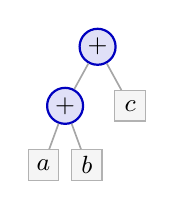
\begin{tikzpicture}[x=0.55cm,y=0.75cm,baseline=(n0.base)]
\node[draw=cA,fill=cA!12,line width=0.8pt,circle,inner sep=1.2pt,minimum size=13pt,font=\small] (n0) at (1.250,0) {$+$};
\node[draw=cA,fill=cA!12,line width=0.8pt,circle,inner sep=1.2pt,minimum size=13pt,font=\small] (n1) at (0.500,-1) {$+$};
\node[draw=gray!60,fill=gray!8,rectangle,inner sep=1.6pt,minimum size=11pt,font=\small] (n2) at (0.000,-2) {$a$};
\node[draw=gray!60,fill=gray!8,rectangle,inner sep=1.6pt,minimum size=11pt,font=\small] (n3) at (1.000,-2) {$b$};
\node[draw=gray!60,fill=gray!8,rectangle,inner sep=1.6pt,minimum size=11pt,font=\small] (n4) at (2.000,-1) {$c$};
\draw[gray!70,line width=0.6pt] (n1) -- (n2);
\draw[gray!70,line width=0.6pt] (n1) -- (n3);
\draw[gray!70,line width=0.6pt] (n0) -- (n1);
\draw[gray!70,line width=0.6pt] (n0) -- (n4);
\end{tikzpicture}\\[4pt]$(a+b)+c\ \to\ {+}{+}abc$\\[2pt]{\small 型 22000}\end{tabular} & \begin{tabular}{c}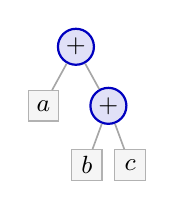
\begin{tikzpicture}[x=0.55cm,y=0.75cm,baseline=(n0.base)]
\node[draw=cA,fill=cA!12,line width=0.8pt,circle,inner sep=1.2pt,minimum size=13pt,font=\small] (n0) at (0.750,0) {$+$};
\node[draw=gray!60,fill=gray!8,rectangle,inner sep=1.6pt,minimum size=11pt,font=\small] (n1) at (0.000,-1) {$a$};
\node[draw=cA,fill=cA!12,line width=0.8pt,circle,inner sep=1.2pt,minimum size=13pt,font=\small] (n2) at (1.500,-1) {$+$};
\node[draw=gray!60,fill=gray!8,rectangle,inner sep=1.6pt,minimum size=11pt,font=\small] (n3) at (1.000,-2) {$b$};
\node[draw=gray!60,fill=gray!8,rectangle,inner sep=1.6pt,minimum size=11pt,font=\small] (n4) at (2.000,-2) {$c$};
\draw[gray!70,line width=0.6pt] (n2) -- (n3);
\draw[gray!70,line width=0.6pt] (n2) -- (n4);
\draw[gray!70,line width=0.6pt] (n0) -- (n1);
\draw[gray!70,line width=0.6pt] (n0) -- (n2);
\end{tikzpicture}\\[4pt]$a+(b+c)\ \to\ {+}a{+}bc$\\[2pt]{\small 型 20200}\end{tabular} & \begin{tabular}{c}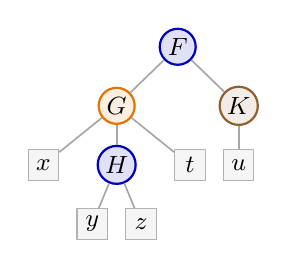
\begin{tikzpicture}[x=0.62cm,y=0.75cm,baseline=(n0.base)]
\node[draw=cA,fill=cA!12,line width=0.8pt,circle,inner sep=1.2pt,minimum size=13pt,font=\small] (n0) at (2.750,0) {$F$};
\node[draw=cB,fill=cB!12,line width=0.8pt,circle,inner sep=1.2pt,minimum size=13pt,font=\small] (n1) at (1.500,-1) {$G$};
\node[draw=gray!60,fill=gray!8,rectangle,inner sep=1.6pt,minimum size=11pt,font=\small] (n2) at (0.000,-2) {$x$};
\node[draw=cA,fill=cA!12,line width=0.8pt,circle,inner sep=1.2pt,minimum size=13pt,font=\small] (n3) at (1.500,-2) {$H$};
\node[draw=gray!60,fill=gray!8,rectangle,inner sep=1.6pt,minimum size=11pt,font=\small] (n4) at (1.000,-3) {$y$};
\node[draw=gray!60,fill=gray!8,rectangle,inner sep=1.6pt,minimum size=11pt,font=\small] (n5) at (2.000,-3) {$z$};
\node[draw=gray!60,fill=gray!8,rectangle,inner sep=1.6pt,minimum size=11pt,font=\small] (n6) at (3.000,-2) {$t$};
\node[draw=cU,fill=cU!12,line width=0.8pt,circle,inner sep=1.2pt,minimum size=13pt,font=\small] (n7) at (4.000,-1) {$K$};
\node[draw=gray!60,fill=gray!8,rectangle,inner sep=1.6pt,minimum size=11pt,font=\small] (n8) at (4.000,-2) {$u$};
\draw[gray!70,line width=0.6pt] (n3) -- (n4);
\draw[gray!70,line width=0.6pt] (n3) -- (n5);
\draw[gray!70,line width=0.6pt] (n1) -- (n2);
\draw[gray!70,line width=0.6pt] (n1) -- (n3);
\draw[gray!70,line width=0.6pt] (n1) -- (n6);
\draw[gray!70,line width=0.6pt] (n7) -- (n8);
\draw[gray!70,line width=0.6pt] (n0) -- (n1);
\draw[gray!70,line width=0.6pt] (n0) -- (n7);
\end{tikzpicture}\\[4pt]$F(G(x,H(y,z),t),K(u))$\\[2pt]{\small 型 230200010}\end{tabular}\end{tabular}}

\newcommand{\RanRankF}{%
\begin{tabular}{@{}lcccccccccc@{}}
開頭的長度 $j$ & 0 & 1 & 2 & 3 & 4 & 5 & 6 & 7 & 8 & 9\\
第 $j$ 個符號 & — & \textcolor{cA}{2} & \textcolor{cB}{3} & \textcolor{gray!70!black}{0} & \textcolor{cA}{2} & \textcolor{gray!70!black}{0} & \textcolor{gray!70!black}{0} & \textcolor{gray!70!black}{0} & \textcolor{cU}{1} & \textcolor{gray!70!black}{0}\\
開頭的秩 & 0 & 1 & 3 & 2 & 3 & 2 & 1 & 0 & 0 & -1\\
\end{tabular}\qquad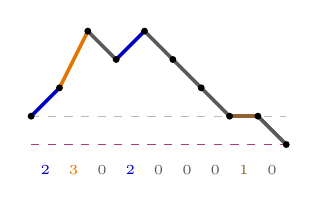
\begin{tikzpicture}[x=0.36cm,y=0.36cm,baseline={([yshift=-0.5ex]current bounding box.center)}]
\draw[gray!55,dashed] (0,0) -- (9,0);
\draw[magenta!70!black,dashed] (0,-1) -- (9,-1);
\draw[cA,line width=1.3pt,line cap=round] (0,0) -- (1,1);
\draw[cB,line width=1.3pt,line cap=round] (1,1) -- (2,3);
\draw[gray!70!black,line width=1.3pt,line cap=round] (2,3) -- (3,2);
\draw[cA,line width=1.3pt,line cap=round] (3,2) -- (4,3);
\draw[gray!70!black,line width=1.3pt,line cap=round] (4,3) -- (5,2);
\draw[gray!70!black,line width=1.3pt,line cap=round] (5,2) -- (6,1);
\draw[gray!70!black,line width=1.3pt,line cap=round] (6,1) -- (7,0);
\draw[cU,line width=1.3pt,line cap=round] (7,0) -- (8,0);
\draw[gray!70!black,line width=1.3pt,line cap=round] (8,0) -- (9,-1);
\fill (0,0) circle (1.25pt);
\fill (1,1) circle (1.25pt);
\fill (2,3) circle (1.25pt);
\fill (3,2) circle (1.25pt);
\fill (4,3) circle (1.25pt);
\fill (5,2) circle (1.25pt);
\fill (6,1) circle (1.25pt);
\fill (7,0) circle (1.25pt);
\fill (8,0) circle (1.25pt);
\fill (9,-1) circle (1.25pt);
\node[font=\tiny,cA] at (0.5,-1.9) {2};
\node[font=\tiny,cB] at (1.5,-1.9) {3};
\node[font=\tiny,gray!70!black] at (2.5,-1.9) {0};
\node[font=\tiny,cA] at (3.5,-1.9) {2};
\node[font=\tiny,gray!70!black] at (4.5,-1.9) {0};
\node[font=\tiny,gray!70!black] at (5.5,-1.9) {0};
\node[font=\tiny,gray!70!black] at (6.5,-1.9) {0};
\node[font=\tiny,cU] at (7.5,-1.9) {1};
\node[font=\tiny,gray!70!black] at (8.5,-1.9) {0};
\end{tikzpicture}}

\newcommand{\RanCayley}{%
\begin{tabular}{ccccc}\begin{tabular}{c}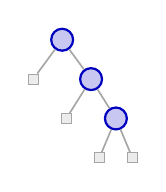
\begin{tikzpicture}[x=0.42cm,y=0.5cm,baseline=(n0.base)]
\node[circle,draw=cA,fill=cA!22,line width=0.8pt,inner sep=2.8pt] (n0) at (0.875,0) {};
\node[rectangle,draw=gray!70,fill=gray!15,inner sep=1.8pt] (n1) at (0.000,-1) {};
\node[circle,draw=cA,fill=cA!22,line width=0.8pt,inner sep=2.8pt] (n2) at (1.750,-1) {};
\node[rectangle,draw=gray!70,fill=gray!15,inner sep=1.8pt] (n3) at (1.000,-2) {};
\node[circle,draw=cA,fill=cA!22,line width=0.8pt,inner sep=2.8pt] (n4) at (2.500,-2) {};
\node[rectangle,draw=gray!70,fill=gray!15,inner sep=1.8pt] (n5) at (2.000,-3) {};
\node[rectangle,draw=gray!70,fill=gray!15,inner sep=1.8pt] (n6) at (3.000,-3) {};
\draw[gray!70,line width=0.6pt] (n4) -- (n5);
\draw[gray!70,line width=0.6pt] (n4) -- (n6);
\draw[gray!70,line width=0.6pt] (n2) -- (n3);
\draw[gray!70,line width=0.6pt] (n2) -- (n4);
\draw[gray!70,line width=0.6pt] (n0) -- (n1);
\draw[gray!70,line width=0.6pt] (n0) -- (n2);
\end{tikzpicture}\\[3pt]$\textcolor{cA}{2}\,\textcolor{gray!70!black}{0}\,\textcolor{cA}{2}\,\textcolor{gray!70!black}{0}\,\textcolor{cA}{2}\,\textcolor{gray!70!black}{0}\,\textcolor{gray!70!black}{0}$\\[1pt]{\small $a(b(cd))$}\end{tabular} & \begin{tabular}{c}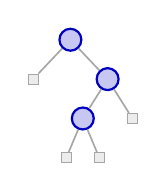
\begin{tikzpicture}[x=0.42cm,y=0.5cm,baseline=(n0.base)]
\node[circle,draw=cA,fill=cA!22,line width=0.8pt,inner sep=2.8pt] (n0) at (1.125,0) {};
\node[rectangle,draw=gray!70,fill=gray!15,inner sep=1.8pt] (n1) at (0.000,-1) {};
\node[circle,draw=cA,fill=cA!22,line width=0.8pt,inner sep=2.8pt] (n2) at (2.250,-1) {};
\node[circle,draw=cA,fill=cA!22,line width=0.8pt,inner sep=2.8pt] (n3) at (1.500,-2) {};
\node[rectangle,draw=gray!70,fill=gray!15,inner sep=1.8pt] (n4) at (1.000,-3) {};
\node[rectangle,draw=gray!70,fill=gray!15,inner sep=1.8pt] (n5) at (2.000,-3) {};
\node[rectangle,draw=gray!70,fill=gray!15,inner sep=1.8pt] (n6) at (3.000,-2) {};
\draw[gray!70,line width=0.6pt] (n3) -- (n4);
\draw[gray!70,line width=0.6pt] (n3) -- (n5);
\draw[gray!70,line width=0.6pt] (n2) -- (n3);
\draw[gray!70,line width=0.6pt] (n2) -- (n6);
\draw[gray!70,line width=0.6pt] (n0) -- (n1);
\draw[gray!70,line width=0.6pt] (n0) -- (n2);
\end{tikzpicture}\\[3pt]$\textcolor{cA}{2}\,\textcolor{gray!70!black}{0}\,\textcolor{cA}{2}\,\textcolor{cA}{2}\,\textcolor{gray!70!black}{0}\,\textcolor{gray!70!black}{0}\,\textcolor{gray!70!black}{0}$\\[1pt]{\small $a((bc)d)$}\end{tabular} & \begin{tabular}{c}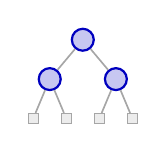
\begin{tikzpicture}[x=0.42cm,y=0.5cm,baseline=(n0.base)]
\node[circle,draw=cA,fill=cA!22,line width=0.8pt,inner sep=2.8pt] (n0) at (1.500,0) {};
\node[circle,draw=cA,fill=cA!22,line width=0.8pt,inner sep=2.8pt] (n1) at (0.500,-1) {};
\node[rectangle,draw=gray!70,fill=gray!15,inner sep=1.8pt] (n2) at (0.000,-2) {};
\node[rectangle,draw=gray!70,fill=gray!15,inner sep=1.8pt] (n3) at (1.000,-2) {};
\node[circle,draw=cA,fill=cA!22,line width=0.8pt,inner sep=2.8pt] (n4) at (2.500,-1) {};
\node[rectangle,draw=gray!70,fill=gray!15,inner sep=1.8pt] (n5) at (2.000,-2) {};
\node[rectangle,draw=gray!70,fill=gray!15,inner sep=1.8pt] (n6) at (3.000,-2) {};
\draw[gray!70,line width=0.6pt] (n1) -- (n2);
\draw[gray!70,line width=0.6pt] (n1) -- (n3);
\draw[gray!70,line width=0.6pt] (n4) -- (n5);
\draw[gray!70,line width=0.6pt] (n4) -- (n6);
\draw[gray!70,line width=0.6pt] (n0) -- (n1);
\draw[gray!70,line width=0.6pt] (n0) -- (n4);
\end{tikzpicture}\\[3pt]$\textcolor{cA}{2}\,\textcolor{cA}{2}\,\textcolor{gray!70!black}{0}\,\textcolor{gray!70!black}{0}\,\textcolor{cA}{2}\,\textcolor{gray!70!black}{0}\,\textcolor{gray!70!black}{0}$\\[1pt]{\small $(ab)(cd)$}\end{tabular} & \begin{tabular}{c}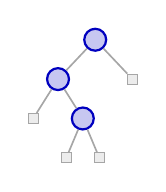
\begin{tikzpicture}[x=0.42cm,y=0.5cm,baseline=(n0.base)]
\node[circle,draw=cA,fill=cA!22,line width=0.8pt,inner sep=2.8pt] (n0) at (1.875,0) {};
\node[circle,draw=cA,fill=cA!22,line width=0.8pt,inner sep=2.8pt] (n1) at (0.750,-1) {};
\node[rectangle,draw=gray!70,fill=gray!15,inner sep=1.8pt] (n2) at (0.000,-2) {};
\node[circle,draw=cA,fill=cA!22,line width=0.8pt,inner sep=2.8pt] (n3) at (1.500,-2) {};
\node[rectangle,draw=gray!70,fill=gray!15,inner sep=1.8pt] (n4) at (1.000,-3) {};
\node[rectangle,draw=gray!70,fill=gray!15,inner sep=1.8pt] (n5) at (2.000,-3) {};
\node[rectangle,draw=gray!70,fill=gray!15,inner sep=1.8pt] (n6) at (3.000,-1) {};
\draw[gray!70,line width=0.6pt] (n3) -- (n4);
\draw[gray!70,line width=0.6pt] (n3) -- (n5);
\draw[gray!70,line width=0.6pt] (n1) -- (n2);
\draw[gray!70,line width=0.6pt] (n1) -- (n3);
\draw[gray!70,line width=0.6pt] (n0) -- (n1);
\draw[gray!70,line width=0.6pt] (n0) -- (n6);
\end{tikzpicture}\\[3pt]$\textcolor{cA}{2}\,\textcolor{cA}{2}\,\textcolor{gray!70!black}{0}\,\textcolor{cA}{2}\,\textcolor{gray!70!black}{0}\,\textcolor{gray!70!black}{0}\,\textcolor{gray!70!black}{0}$\\[1pt]{\small $(a(bc))d$}\end{tabular} & \begin{tabular}{c}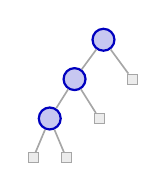
\begin{tikzpicture}[x=0.42cm,y=0.5cm,baseline=(n0.base)]
\node[circle,draw=cA,fill=cA!22,line width=0.8pt,inner sep=2.8pt] (n0) at (2.125,0) {};
\node[circle,draw=cA,fill=cA!22,line width=0.8pt,inner sep=2.8pt] (n1) at (1.250,-1) {};
\node[circle,draw=cA,fill=cA!22,line width=0.8pt,inner sep=2.8pt] (n2) at (0.500,-2) {};
\node[rectangle,draw=gray!70,fill=gray!15,inner sep=1.8pt] (n3) at (0.000,-3) {};
\node[rectangle,draw=gray!70,fill=gray!15,inner sep=1.8pt] (n4) at (1.000,-3) {};
\node[rectangle,draw=gray!70,fill=gray!15,inner sep=1.8pt] (n5) at (2.000,-2) {};
\node[rectangle,draw=gray!70,fill=gray!15,inner sep=1.8pt] (n6) at (3.000,-1) {};
\draw[gray!70,line width=0.6pt] (n2) -- (n3);
\draw[gray!70,line width=0.6pt] (n2) -- (n4);
\draw[gray!70,line width=0.6pt] (n1) -- (n2);
\draw[gray!70,line width=0.6pt] (n1) -- (n5);
\draw[gray!70,line width=0.6pt] (n0) -- (n1);
\draw[gray!70,line width=0.6pt] (n0) -- (n6);
\end{tikzpicture}\\[3pt]$\textcolor{cA}{2}\,\textcolor{cA}{2}\,\textcolor{cA}{2}\,\textcolor{gray!70!black}{0}\,\textcolor{gray!70!black}{0}\,\textcolor{gray!70!black}{0}\,\textcolor{gray!70!black}{0}$\\[1pt]{\small $((ab)c)d$}\end{tabular}\end{tabular}}

\newcommand{\RanChuFigOne}{%
\begin{tabular}{ccccc}\begin{tabular}{c}\PaperCfgRoot{4}{5}{1}{2}{3}\\[3pt]$\textcolor{cB}{3}\,\textcolor{gray!70!black}{0}\,\textcolor{gray!70!black}{0}\,\textcolor{cA}{2}\,\textcolor{gray!70!black}{0}\,\textcolor{gray!70!black}{0}$\\[3pt]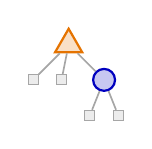
\begin{tikzpicture}[x=0.36cm,y=0.45cm,baseline=(n0.base)]
\node[regular polygon,regular polygon sides=3,draw=cB,fill=cB!22,line width=0.8pt,inner sep=2.0pt] (n0) at (1.250,0) {};
\node[rectangle,draw=gray!70,fill=gray!15,inner sep=1.8pt] (n1) at (0.000,-1) {};
\node[rectangle,draw=gray!70,fill=gray!15,inner sep=1.8pt] (n2) at (1.000,-1) {};
\node[circle,draw=cA,fill=cA!22,line width=0.8pt,inner sep=2.8pt] (n3) at (2.500,-1) {};
\node[rectangle,draw=gray!70,fill=gray!15,inner sep=1.8pt] (n4) at (2.000,-2) {};
\node[rectangle,draw=gray!70,fill=gray!15,inner sep=1.8pt] (n5) at (3.000,-2) {};
\draw[gray!70,line width=0.6pt] (n3) -- (n4);
\draw[gray!70,line width=0.6pt] (n3) -- (n5);
\draw[gray!70,line width=0.6pt] (n0) -- (n1);
\draw[gray!70,line width=0.6pt] (n0) -- (n2);
\draw[gray!70,line width=0.6pt] (n0) -- (n3);
\end{tikzpicture}\end{tabular} & \begin{tabular}{c}\PaperCfgRoot{5}{1}{2}{3}{4}\\[3pt]$\textcolor{cA}{2}\,\textcolor{cB}{3}\,\textcolor{gray!70!black}{0}\,\textcolor{gray!70!black}{0}\,\textcolor{gray!70!black}{0}\,\textcolor{gray!70!black}{0}$\\[3pt]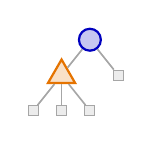
\begin{tikzpicture}[x=0.36cm,y=0.45cm,baseline=(n0.base)]
\node[circle,draw=cA,fill=cA!22,line width=0.8pt,inner sep=2.8pt] (n0) at (2.000,0) {};
\node[regular polygon,regular polygon sides=3,draw=cB,fill=cB!22,line width=0.8pt,inner sep=2.0pt] (n1) at (1.000,-1) {};
\node[rectangle,draw=gray!70,fill=gray!15,inner sep=1.8pt] (n2) at (0.000,-2) {};
\node[rectangle,draw=gray!70,fill=gray!15,inner sep=1.8pt] (n3) at (1.000,-2) {};
\node[rectangle,draw=gray!70,fill=gray!15,inner sep=1.8pt] (n4) at (2.000,-2) {};
\node[rectangle,draw=gray!70,fill=gray!15,inner sep=1.8pt] (n5) at (3.000,-1) {};
\draw[gray!70,line width=0.6pt] (n1) -- (n2);
\draw[gray!70,line width=0.6pt] (n1) -- (n3);
\draw[gray!70,line width=0.6pt] (n1) -- (n4);
\draw[gray!70,line width=0.6pt] (n0) -- (n1);
\draw[gray!70,line width=0.6pt] (n0) -- (n5);
\end{tikzpicture}\end{tabular} & \begin{tabular}{c}\PaperCfgRoot{1}{2}{3}{4}{5}\\[3pt]$\textcolor{cA}{2}\,\textcolor{gray!70!black}{0}\,\textcolor{cB}{3}\,\textcolor{gray!70!black}{0}\,\textcolor{gray!70!black}{0}\,\textcolor{gray!70!black}{0}$\\[3pt]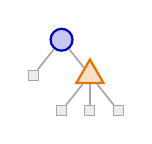
\begin{tikzpicture}[x=0.36cm,y=0.45cm,baseline=(n0.base)]
\node[circle,draw=cA,fill=cA!22,line width=0.8pt,inner sep=2.8pt] (n0) at (1.000,0) {};
\node[rectangle,draw=gray!70,fill=gray!15,inner sep=1.8pt] (n1) at (0.000,-1) {};
\node[regular polygon,regular polygon sides=3,draw=cB,fill=cB!22,line width=0.8pt,inner sep=2.0pt] (n2) at (2.000,-1) {};
\node[rectangle,draw=gray!70,fill=gray!15,inner sep=1.8pt] (n3) at (1.000,-2) {};
\node[rectangle,draw=gray!70,fill=gray!15,inner sep=1.8pt] (n4) at (2.000,-2) {};
\node[rectangle,draw=gray!70,fill=gray!15,inner sep=1.8pt] (n5) at (3.000,-2) {};
\draw[gray!70,line width=0.6pt] (n2) -- (n3);
\draw[gray!70,line width=0.6pt] (n2) -- (n4);
\draw[gray!70,line width=0.6pt] (n2) -- (n5);
\draw[gray!70,line width=0.6pt] (n0) -- (n1);
\draw[gray!70,line width=0.6pt] (n0) -- (n2);
\end{tikzpicture}\end{tabular} & \begin{tabular}{c}\PaperCfgRoot{2}{3}{4}{5}{1}\\[3pt]$\textcolor{cB}{3}\,\textcolor{cA}{2}\,\textcolor{gray!70!black}{0}\,\textcolor{gray!70!black}{0}\,\textcolor{gray!70!black}{0}\,\textcolor{gray!70!black}{0}$\\[3pt]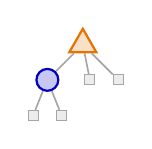
\begin{tikzpicture}[x=0.36cm,y=0.45cm,baseline=(n0.base)]
\node[regular polygon,regular polygon sides=3,draw=cB,fill=cB!22,line width=0.8pt,inner sep=2.0pt] (n0) at (1.750,0) {};
\node[circle,draw=cA,fill=cA!22,line width=0.8pt,inner sep=2.8pt] (n1) at (0.500,-1) {};
\node[rectangle,draw=gray!70,fill=gray!15,inner sep=1.8pt] (n2) at (0.000,-2) {};
\node[rectangle,draw=gray!70,fill=gray!15,inner sep=1.8pt] (n3) at (1.000,-2) {};
\node[rectangle,draw=gray!70,fill=gray!15,inner sep=1.8pt] (n4) at (2.000,-1) {};
\node[rectangle,draw=gray!70,fill=gray!15,inner sep=1.8pt] (n5) at (3.000,-1) {};
\draw[gray!70,line width=0.6pt] (n1) -- (n2);
\draw[gray!70,line width=0.6pt] (n1) -- (n3);
\draw[gray!70,line width=0.6pt] (n0) -- (n1);
\draw[gray!70,line width=0.6pt] (n0) -- (n4);
\draw[gray!70,line width=0.6pt] (n0) -- (n5);
\end{tikzpicture}\end{tabular} & \begin{tabular}{c}\PaperCfgRoot{3}{4}{5}{1}{2}\\[3pt]$\textcolor{cB}{3}\,\textcolor{gray!70!black}{0}\,\textcolor{cA}{2}\,\textcolor{gray!70!black}{0}\,\textcolor{gray!70!black}{0}\,\textcolor{gray!70!black}{0}$\\[3pt]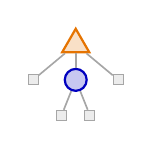
\begin{tikzpicture}[x=0.36cm,y=0.45cm,baseline=(n0.base)]
\node[regular polygon,regular polygon sides=3,draw=cB,fill=cB!22,line width=0.8pt,inner sep=2.0pt] (n0) at (1.500,0) {};
\node[rectangle,draw=gray!70,fill=gray!15,inner sep=1.8pt] (n1) at (0.000,-1) {};
\node[circle,draw=cA,fill=cA!22,line width=0.8pt,inner sep=2.8pt] (n2) at (1.500,-1) {};
\node[rectangle,draw=gray!70,fill=gray!15,inner sep=1.8pt] (n3) at (1.000,-2) {};
\node[rectangle,draw=gray!70,fill=gray!15,inner sep=1.8pt] (n4) at (2.000,-2) {};
\node[rectangle,draw=gray!70,fill=gray!15,inner sep=1.8pt] (n5) at (3.000,-1) {};
\draw[gray!70,line width=0.6pt] (n2) -- (n3);
\draw[gray!70,line width=0.6pt] (n2) -- (n4);
\draw[gray!70,line width=0.6pt] (n0) -- (n1);
\draw[gray!70,line width=0.6pt] (n0) -- (n2);
\draw[gray!70,line width=0.6pt] (n0) -- (n5);
\end{tikzpicture}\end{tabular}\end{tabular}}

\newcommand{\RanCycOne}{%
\begin{tabular}{c c c c}\toprule $k$ & $\sigma g_k$ & 秩路徑 & $n$ 字列？\\\midrule
0 & $\textcolor{gray!70!black}{0}\,\textcolor{gray!70!black}{0}\,\textcolor{cA}{2}\,\textcolor{gray!70!black}{0}\,\textcolor{cA}{2}$ & 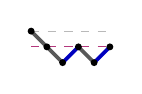
\begin{tikzpicture}[x=0.2cm,y=0.2cm,baseline={([yshift=-0.5ex]current bounding box.center)}]
\draw[gray!55,dashed] (0,0) -- (5,0);
\draw[magenta!70!black,dashed] (0,-1) -- (5,-1);
\draw[gray!70!black,line width=1.3pt,line cap=round] (0,0) -- (1,-1);
\draw[gray!70!black,line width=1.3pt,line cap=round] (1,-1) -- (2,-2);
\draw[cA,line width=1.3pt,line cap=round] (2,-2) -- (3,-1);
\draw[gray!70!black,line width=1.3pt,line cap=round] (3,-1) -- (4,-2);
\draw[cA,line width=1.3pt,line cap=round] (4,-2) -- (5,-1);
\fill (0,0) circle (1.25pt);
\fill (1,-1) circle (1.25pt);
\fill (2,-2) circle (1.25pt);
\fill (3,-1) circle (1.25pt);
\fill (4,-2) circle (1.25pt);
\fill (5,-1) circle (1.25pt);
\end{tikzpicture} & \textcolor{cBad}{$\times$}\\[2pt]
1 & $\textcolor{gray!70!black}{0}\,\textcolor{cA}{2}\,\textcolor{gray!70!black}{0}\,\textcolor{cA}{2}\,\textcolor{gray!70!black}{0}$ & 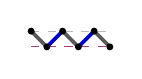
\begin{tikzpicture}[x=0.2cm,y=0.2cm,baseline={([yshift=-0.5ex]current bounding box.center)}]
\draw[gray!55,dashed] (0,0) -- (5,0);
\draw[magenta!70!black,dashed] (0,-1) -- (5,-1);
\draw[gray!70!black,line width=1.3pt,line cap=round] (0,0) -- (1,-1);
\draw[cA,line width=1.3pt,line cap=round] (1,-1) -- (2,0);
\draw[gray!70!black,line width=1.3pt,line cap=round] (2,0) -- (3,-1);
\draw[cA,line width=1.3pt,line cap=round] (3,-1) -- (4,0);
\draw[gray!70!black,line width=1.3pt,line cap=round] (4,0) -- (5,-1);
\fill (0,0) circle (1.25pt);
\fill (1,-1) circle (1.25pt);
\fill (2,0) circle (1.25pt);
\fill (3,-1) circle (1.25pt);
\fill (4,0) circle (1.25pt);
\fill (5,-1) circle (1.25pt);
\end{tikzpicture} & \textcolor{cBad}{$\times$}\\[2pt]
2 & $\textcolor{cA}{2}\,\textcolor{gray!70!black}{0}\,\textcolor{cA}{2}\,\textcolor{gray!70!black}{0}\,\textcolor{gray!70!black}{0}$ & 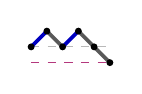
\begin{tikzpicture}[x=0.2cm,y=0.2cm,baseline={([yshift=-0.5ex]current bounding box.center)}]
\draw[gray!55,dashed] (0,0) -- (5,0);
\draw[magenta!70!black,dashed] (0,-1) -- (5,-1);
\draw[cA,line width=1.3pt,line cap=round] (0,0) -- (1,1);
\draw[gray!70!black,line width=1.3pt,line cap=round] (1,1) -- (2,0);
\draw[cA,line width=1.3pt,line cap=round] (2,0) -- (3,1);
\draw[gray!70!black,line width=1.3pt,line cap=round] (3,1) -- (4,0);
\draw[gray!70!black,line width=1.3pt,line cap=round] (4,0) -- (5,-1);
\fill (0,0) circle (1.25pt);
\fill (1,1) circle (1.25pt);
\fill (2,0) circle (1.25pt);
\fill (3,1) circle (1.25pt);
\fill (4,0) circle (1.25pt);
\fill (5,-1) circle (1.25pt);
\end{tikzpicture} & \textcolor{green!50!black}{\checkmark}\\[2pt]
3 & $\textcolor{gray!70!black}{0}\,\textcolor{cA}{2}\,\textcolor{gray!70!black}{0}\,\textcolor{gray!70!black}{0}\,\textcolor{cA}{2}$ & 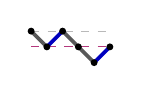
\begin{tikzpicture}[x=0.2cm,y=0.2cm,baseline={([yshift=-0.5ex]current bounding box.center)}]
\draw[gray!55,dashed] (0,0) -- (5,0);
\draw[magenta!70!black,dashed] (0,-1) -- (5,-1);
\draw[gray!70!black,line width=1.3pt,line cap=round] (0,0) -- (1,-1);
\draw[cA,line width=1.3pt,line cap=round] (1,-1) -- (2,0);
\draw[gray!70!black,line width=1.3pt,line cap=round] (2,0) -- (3,-1);
\draw[gray!70!black,line width=1.3pt,line cap=round] (3,-1) -- (4,-2);
\draw[cA,line width=1.3pt,line cap=round] (4,-2) -- (5,-1);
\fill (0,0) circle (1.25pt);
\fill (1,-1) circle (1.25pt);
\fill (2,0) circle (1.25pt);
\fill (3,-1) circle (1.25pt);
\fill (4,-2) circle (1.25pt);
\fill (5,-1) circle (1.25pt);
\end{tikzpicture} & \textcolor{cBad}{$\times$}\\[2pt]
4 & $\textcolor{cA}{2}\,\textcolor{gray!70!black}{0}\,\textcolor{gray!70!black}{0}\,\textcolor{cA}{2}\,\textcolor{gray!70!black}{0}$ & 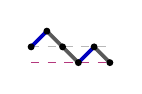
\begin{tikzpicture}[x=0.2cm,y=0.2cm,baseline={([yshift=-0.5ex]current bounding box.center)}]
\draw[gray!55,dashed] (0,0) -- (5,0);
\draw[magenta!70!black,dashed] (0,-1) -- (5,-1);
\draw[cA,line width=1.3pt,line cap=round] (0,0) -- (1,1);
\draw[gray!70!black,line width=1.3pt,line cap=round] (1,1) -- (2,0);
\draw[gray!70!black,line width=1.3pt,line cap=round] (2,0) -- (3,-1);
\draw[cA,line width=1.3pt,line cap=round] (3,-1) -- (4,0);
\draw[gray!70!black,line width=1.3pt,line cap=round] (4,0) -- (5,-1);
\fill (0,0) circle (1.25pt);
\fill (1,1) circle (1.25pt);
\fill (2,0) circle (1.25pt);
\fill (3,-1) circle (1.25pt);
\fill (4,0) circle (1.25pt);
\fill (5,-1) circle (1.25pt);
\end{tikzpicture} & \textcolor{cBad}{$\times$}\\[2pt]\bottomrule\end{tabular}}

\newcommand{\RanCycTwo}{%
\begin{tabular}{c c c c c}\toprule $k$ & $\sigma g_k$ & 秩路徑 & Chu 講義的路徑 & $n$ 字列？\\\midrule
0 & $\textcolor{gray!70!black}{0}\,\textcolor{gray!70!black}{0}\,\textcolor{cA}{2}\,\textcolor{gray!70!black}{0}\,\textcolor{gray!70!black}{0}\,\textcolor{cB}{3}\,\textcolor{gray!70!black}{0}$ & 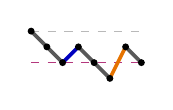
\begin{tikzpicture}[x=0.2cm,y=0.2cm,baseline={([yshift=-0.5ex]current bounding box.center)}]
\draw[gray!55,dashed] (0,0) -- (7,0);
\draw[magenta!70!black,dashed] (0,-2) -- (7,-2);
\draw[gray!70!black,line width=1.3pt,line cap=round] (0,0) -- (1,-1);
\draw[gray!70!black,line width=1.3pt,line cap=round] (1,-1) -- (2,-2);
\draw[cA,line width=1.3pt,line cap=round] (2,-2) -- (3,-1);
\draw[gray!70!black,line width=1.3pt,line cap=round] (3,-1) -- (4,-2);
\draw[gray!70!black,line width=1.3pt,line cap=round] (4,-2) -- (5,-3);
\draw[cB,line width=1.3pt,line cap=round] (5,-3) -- (6,-1);
\draw[gray!70!black,line width=1.3pt,line cap=round] (6,-1) -- (7,-2);
\fill (0,0) circle (1.25pt);
\fill (1,-1) circle (1.25pt);
\fill (2,-2) circle (1.25pt);
\fill (3,-1) circle (1.25pt);
\fill (4,-2) circle (1.25pt);
\fill (5,-3) circle (1.25pt);
\fill (6,-1) circle (1.25pt);
\fill (7,-2) circle (1.25pt);
\end{tikzpicture} & 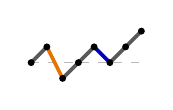
\begin{tikzpicture}[x=0.2cm,y=0.2cm,baseline={([yshift=-0.5ex]current bounding box.center)}]
\draw[gray!55,dashed] (0,0) -- (7,0);
\draw[gray!70!black,line width=1.3pt,line cap=round] (0,0) -- (1,1);
\draw[cB,line width=1.3pt,line cap=round] (1,1) -- (2,-1);
\draw[gray!70!black,line width=1.3pt,line cap=round] (2,-1) -- (3,0);
\draw[gray!70!black,line width=1.3pt,line cap=round] (3,0) -- (4,1);
\draw[cA,line width=1.3pt,line cap=round] (4,1) -- (5,0);
\draw[gray!70!black,line width=1.3pt,line cap=round] (5,0) -- (6,1);
\draw[gray!70!black,line width=1.3pt,line cap=round] (6,1) -- (7,2);
\fill (0,0) circle (1.25pt);
\fill (1,1) circle (1.25pt);
\fill (2,-1) circle (1.25pt);
\fill (3,0) circle (1.25pt);
\fill (4,1) circle (1.25pt);
\fill (5,0) circle (1.25pt);
\fill (6,1) circle (1.25pt);
\fill (7,2) circle (1.25pt);
\end{tikzpicture} & \textcolor{cBad}{$\times$}\\[2pt]
1 & $\textcolor{gray!70!black}{0}\,\textcolor{cA}{2}\,\textcolor{gray!70!black}{0}\,\textcolor{gray!70!black}{0}\,\textcolor{cB}{3}\,\textcolor{gray!70!black}{0}\,\textcolor{gray!70!black}{0}$ & 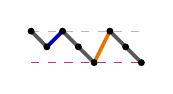
\begin{tikzpicture}[x=0.2cm,y=0.2cm,baseline={([yshift=-0.5ex]current bounding box.center)}]
\draw[gray!55,dashed] (0,0) -- (7,0);
\draw[magenta!70!black,dashed] (0,-2) -- (7,-2);
\draw[gray!70!black,line width=1.3pt,line cap=round] (0,0) -- (1,-1);
\draw[cA,line width=1.3pt,line cap=round] (1,-1) -- (2,0);
\draw[gray!70!black,line width=1.3pt,line cap=round] (2,0) -- (3,-1);
\draw[gray!70!black,line width=1.3pt,line cap=round] (3,-1) -- (4,-2);
\draw[cB,line width=1.3pt,line cap=round] (4,-2) -- (5,0);
\draw[gray!70!black,line width=1.3pt,line cap=round] (5,0) -- (6,-1);
\draw[gray!70!black,line width=1.3pt,line cap=round] (6,-1) -- (7,-2);
\fill (0,0) circle (1.25pt);
\fill (1,-1) circle (1.25pt);
\fill (2,0) circle (1.25pt);
\fill (3,-1) circle (1.25pt);
\fill (4,-2) circle (1.25pt);
\fill (5,0) circle (1.25pt);
\fill (6,-1) circle (1.25pt);
\fill (7,-2) circle (1.25pt);
\end{tikzpicture} & 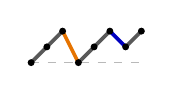
\begin{tikzpicture}[x=0.2cm,y=0.2cm,baseline={([yshift=-0.5ex]current bounding box.center)}]
\draw[gray!55,dashed] (0,0) -- (7,0);
\draw[gray!70!black,line width=1.3pt,line cap=round] (0,0) -- (1,1);
\draw[gray!70!black,line width=1.3pt,line cap=round] (1,1) -- (2,2);
\draw[cB,line width=1.3pt,line cap=round] (2,2) -- (3,0);
\draw[gray!70!black,line width=1.3pt,line cap=round] (3,0) -- (4,1);
\draw[gray!70!black,line width=1.3pt,line cap=round] (4,1) -- (5,2);
\draw[cA,line width=1.3pt,line cap=round] (5,2) -- (6,1);
\draw[gray!70!black,line width=1.3pt,line cap=round] (6,1) -- (7,2);
\fill (0,0) circle (1.25pt);
\fill (1,1) circle (1.25pt);
\fill (2,2) circle (1.25pt);
\fill (3,0) circle (1.25pt);
\fill (4,1) circle (1.25pt);
\fill (5,2) circle (1.25pt);
\fill (6,1) circle (1.25pt);
\fill (7,2) circle (1.25pt);
\end{tikzpicture} & \textcolor{cBad}{$\times$}\\[2pt]
2 & $\textcolor{cA}{2}\,\textcolor{gray!70!black}{0}\,\textcolor{gray!70!black}{0}\,\textcolor{cB}{3}\,\textcolor{gray!70!black}{0}\,\textcolor{gray!70!black}{0}\,\textcolor{gray!70!black}{0}$ & 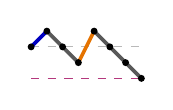
\begin{tikzpicture}[x=0.2cm,y=0.2cm,baseline={([yshift=-0.5ex]current bounding box.center)}]
\draw[gray!55,dashed] (0,0) -- (7,0);
\draw[magenta!70!black,dashed] (0,-2) -- (7,-2);
\draw[cA,line width=1.3pt,line cap=round] (0,0) -- (1,1);
\draw[gray!70!black,line width=1.3pt,line cap=round] (1,1) -- (2,0);
\draw[gray!70!black,line width=1.3pt,line cap=round] (2,0) -- (3,-1);
\draw[cB,line width=1.3pt,line cap=round] (3,-1) -- (4,1);
\draw[gray!70!black,line width=1.3pt,line cap=round] (4,1) -- (5,0);
\draw[gray!70!black,line width=1.3pt,line cap=round] (5,0) -- (6,-1);
\draw[gray!70!black,line width=1.3pt,line cap=round] (6,-1) -- (7,-2);
\fill (0,0) circle (1.25pt);
\fill (1,1) circle (1.25pt);
\fill (2,0) circle (1.25pt);
\fill (3,-1) circle (1.25pt);
\fill (4,1) circle (1.25pt);
\fill (5,0) circle (1.25pt);
\fill (6,-1) circle (1.25pt);
\fill (7,-2) circle (1.25pt);
\end{tikzpicture} & 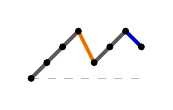
\begin{tikzpicture}[x=0.2cm,y=0.2cm,baseline={([yshift=-0.5ex]current bounding box.center)}]
\draw[gray!55,dashed] (0,0) -- (7,0);
\draw[gray!70!black,line width=1.3pt,line cap=round] (0,0) -- (1,1);
\draw[gray!70!black,line width=1.3pt,line cap=round] (1,1) -- (2,2);
\draw[gray!70!black,line width=1.3pt,line cap=round] (2,2) -- (3,3);
\draw[cB,line width=1.3pt,line cap=round] (3,3) -- (4,1);
\draw[gray!70!black,line width=1.3pt,line cap=round] (4,1) -- (5,2);
\draw[gray!70!black,line width=1.3pt,line cap=round] (5,2) -- (6,3);
\draw[cA,line width=1.3pt,line cap=round] (6,3) -- (7,2);
\fill (0,0) circle (1.25pt);
\fill (1,1) circle (1.25pt);
\fill (2,2) circle (1.25pt);
\fill (3,3) circle (1.25pt);
\fill (4,1) circle (1.25pt);
\fill (5,2) circle (1.25pt);
\fill (6,3) circle (1.25pt);
\fill (7,2) circle (1.25pt);
\end{tikzpicture} & \textcolor{green!50!black}{\checkmark}\\[2pt]
3 & $\textcolor{gray!70!black}{0}\,\textcolor{gray!70!black}{0}\,\textcolor{cB}{3}\,\textcolor{gray!70!black}{0}\,\textcolor{gray!70!black}{0}\,\textcolor{gray!70!black}{0}\,\textcolor{cA}{2}$ & 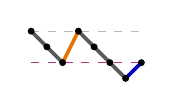
\begin{tikzpicture}[x=0.2cm,y=0.2cm,baseline={([yshift=-0.5ex]current bounding box.center)}]
\draw[gray!55,dashed] (0,0) -- (7,0);
\draw[magenta!70!black,dashed] (0,-2) -- (7,-2);
\draw[gray!70!black,line width=1.3pt,line cap=round] (0,0) -- (1,-1);
\draw[gray!70!black,line width=1.3pt,line cap=round] (1,-1) -- (2,-2);
\draw[cB,line width=1.3pt,line cap=round] (2,-2) -- (3,0);
\draw[gray!70!black,line width=1.3pt,line cap=round] (3,0) -- (4,-1);
\draw[gray!70!black,line width=1.3pt,line cap=round] (4,-1) -- (5,-2);
\draw[gray!70!black,line width=1.3pt,line cap=round] (5,-2) -- (6,-3);
\draw[cA,line width=1.3pt,line cap=round] (6,-3) -- (7,-2);
\fill (0,0) circle (1.25pt);
\fill (1,-1) circle (1.25pt);
\fill (2,-2) circle (1.25pt);
\fill (3,0) circle (1.25pt);
\fill (4,-1) circle (1.25pt);
\fill (5,-2) circle (1.25pt);
\fill (6,-3) circle (1.25pt);
\fill (7,-2) circle (1.25pt);
\end{tikzpicture} & 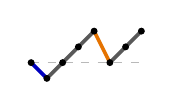
\begin{tikzpicture}[x=0.2cm,y=0.2cm,baseline={([yshift=-0.5ex]current bounding box.center)}]
\draw[gray!55,dashed] (0,0) -- (7,0);
\draw[cA,line width=1.3pt,line cap=round] (0,0) -- (1,-1);
\draw[gray!70!black,line width=1.3pt,line cap=round] (1,-1) -- (2,0);
\draw[gray!70!black,line width=1.3pt,line cap=round] (2,0) -- (3,1);
\draw[gray!70!black,line width=1.3pt,line cap=round] (3,1) -- (4,2);
\draw[cB,line width=1.3pt,line cap=round] (4,2) -- (5,0);
\draw[gray!70!black,line width=1.3pt,line cap=round] (5,0) -- (6,1);
\draw[gray!70!black,line width=1.3pt,line cap=round] (6,1) -- (7,2);
\fill (0,0) circle (1.25pt);
\fill (1,-1) circle (1.25pt);
\fill (2,0) circle (1.25pt);
\fill (3,1) circle (1.25pt);
\fill (4,2) circle (1.25pt);
\fill (5,0) circle (1.25pt);
\fill (6,1) circle (1.25pt);
\fill (7,2) circle (1.25pt);
\end{tikzpicture} & \textcolor{cBad}{$\times$}\\[2pt]
4 & $\textcolor{gray!70!black}{0}\,\textcolor{cB}{3}\,\textcolor{gray!70!black}{0}\,\textcolor{gray!70!black}{0}\,\textcolor{gray!70!black}{0}\,\textcolor{cA}{2}\,\textcolor{gray!70!black}{0}$ & 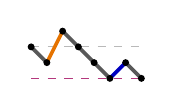
\begin{tikzpicture}[x=0.2cm,y=0.2cm,baseline={([yshift=-0.5ex]current bounding box.center)}]
\draw[gray!55,dashed] (0,0) -- (7,0);
\draw[magenta!70!black,dashed] (0,-2) -- (7,-2);
\draw[gray!70!black,line width=1.3pt,line cap=round] (0,0) -- (1,-1);
\draw[cB,line width=1.3pt,line cap=round] (1,-1) -- (2,1);
\draw[gray!70!black,line width=1.3pt,line cap=round] (2,1) -- (3,0);
\draw[gray!70!black,line width=1.3pt,line cap=round] (3,0) -- (4,-1);
\draw[gray!70!black,line width=1.3pt,line cap=round] (4,-1) -- (5,-2);
\draw[cA,line width=1.3pt,line cap=round] (5,-2) -- (6,-1);
\draw[gray!70!black,line width=1.3pt,line cap=round] (6,-1) -- (7,-2);
\fill (0,0) circle (1.25pt);
\fill (1,-1) circle (1.25pt);
\fill (2,1) circle (1.25pt);
\fill (3,0) circle (1.25pt);
\fill (4,-1) circle (1.25pt);
\fill (5,-2) circle (1.25pt);
\fill (6,-1) circle (1.25pt);
\fill (7,-2) circle (1.25pt);
\end{tikzpicture} & 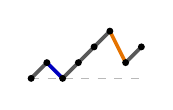
\begin{tikzpicture}[x=0.2cm,y=0.2cm,baseline={([yshift=-0.5ex]current bounding box.center)}]
\draw[gray!55,dashed] (0,0) -- (7,0);
\draw[gray!70!black,line width=1.3pt,line cap=round] (0,0) -- (1,1);
\draw[cA,line width=1.3pt,line cap=round] (1,1) -- (2,0);
\draw[gray!70!black,line width=1.3pt,line cap=round] (2,0) -- (3,1);
\draw[gray!70!black,line width=1.3pt,line cap=round] (3,1) -- (4,2);
\draw[gray!70!black,line width=1.3pt,line cap=round] (4,2) -- (5,3);
\draw[cB,line width=1.3pt,line cap=round] (5,3) -- (6,1);
\draw[gray!70!black,line width=1.3pt,line cap=round] (6,1) -- (7,2);
\fill (0,0) circle (1.25pt);
\fill (1,1) circle (1.25pt);
\fill (2,0) circle (1.25pt);
\fill (3,1) circle (1.25pt);
\fill (4,2) circle (1.25pt);
\fill (5,3) circle (1.25pt);
\fill (6,1) circle (1.25pt);
\fill (7,2) circle (1.25pt);
\end{tikzpicture} & \textcolor{cBad}{$\times$}\\[2pt]
5 & $\textcolor{cB}{3}\,\textcolor{gray!70!black}{0}\,\textcolor{gray!70!black}{0}\,\textcolor{gray!70!black}{0}\,\textcolor{cA}{2}\,\textcolor{gray!70!black}{0}\,\textcolor{gray!70!black}{0}$ & 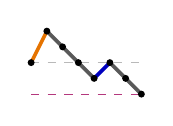
\begin{tikzpicture}[x=0.2cm,y=0.2cm,baseline={([yshift=-0.5ex]current bounding box.center)}]
\draw[gray!55,dashed] (0,0) -- (7,0);
\draw[magenta!70!black,dashed] (0,-2) -- (7,-2);
\draw[cB,line width=1.3pt,line cap=round] (0,0) -- (1,2);
\draw[gray!70!black,line width=1.3pt,line cap=round] (1,2) -- (2,1);
\draw[gray!70!black,line width=1.3pt,line cap=round] (2,1) -- (3,0);
\draw[gray!70!black,line width=1.3pt,line cap=round] (3,0) -- (4,-1);
\draw[cA,line width=1.3pt,line cap=round] (4,-1) -- (5,0);
\draw[gray!70!black,line width=1.3pt,line cap=round] (5,0) -- (6,-1);
\draw[gray!70!black,line width=1.3pt,line cap=round] (6,-1) -- (7,-2);
\fill (0,0) circle (1.25pt);
\fill (1,2) circle (1.25pt);
\fill (2,1) circle (1.25pt);
\fill (3,0) circle (1.25pt);
\fill (4,-1) circle (1.25pt);
\fill (5,0) circle (1.25pt);
\fill (6,-1) circle (1.25pt);
\fill (7,-2) circle (1.25pt);
\end{tikzpicture} & 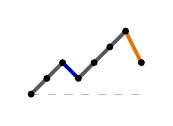
\begin{tikzpicture}[x=0.2cm,y=0.2cm,baseline={([yshift=-0.5ex]current bounding box.center)}]
\draw[gray!55,dashed] (0,0) -- (7,0);
\draw[gray!70!black,line width=1.3pt,line cap=round] (0,0) -- (1,1);
\draw[gray!70!black,line width=1.3pt,line cap=round] (1,1) -- (2,2);
\draw[cA,line width=1.3pt,line cap=round] (2,2) -- (3,1);
\draw[gray!70!black,line width=1.3pt,line cap=round] (3,1) -- (4,2);
\draw[gray!70!black,line width=1.3pt,line cap=round] (4,2) -- (5,3);
\draw[gray!70!black,line width=1.3pt,line cap=round] (5,3) -- (6,4);
\draw[cB,line width=1.3pt,line cap=round] (6,4) -- (7,2);
\fill (0,0) circle (1.25pt);
\fill (1,1) circle (1.25pt);
\fill (2,2) circle (1.25pt);
\fill (3,1) circle (1.25pt);
\fill (4,2) circle (1.25pt);
\fill (5,3) circle (1.25pt);
\fill (6,4) circle (1.25pt);
\fill (7,2) circle (1.25pt);
\end{tikzpicture} & \textcolor{green!50!black}{\checkmark}\\[2pt]
6 & $\textcolor{gray!70!black}{0}\,\textcolor{gray!70!black}{0}\,\textcolor{gray!70!black}{0}\,\textcolor{cA}{2}\,\textcolor{gray!70!black}{0}\,\textcolor{gray!70!black}{0}\,\textcolor{cB}{3}$ & 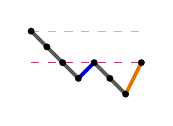
\begin{tikzpicture}[x=0.2cm,y=0.2cm,baseline={([yshift=-0.5ex]current bounding box.center)}]
\draw[gray!55,dashed] (0,0) -- (7,0);
\draw[magenta!70!black,dashed] (0,-2) -- (7,-2);
\draw[gray!70!black,line width=1.3pt,line cap=round] (0,0) -- (1,-1);
\draw[gray!70!black,line width=1.3pt,line cap=round] (1,-1) -- (2,-2);
\draw[gray!70!black,line width=1.3pt,line cap=round] (2,-2) -- (3,-3);
\draw[cA,line width=1.3pt,line cap=round] (3,-3) -- (4,-2);
\draw[gray!70!black,line width=1.3pt,line cap=round] (4,-2) -- (5,-3);
\draw[gray!70!black,line width=1.3pt,line cap=round] (5,-3) -- (6,-4);
\draw[cB,line width=1.3pt,line cap=round] (6,-4) -- (7,-2);
\fill (0,0) circle (1.25pt);
\fill (1,-1) circle (1.25pt);
\fill (2,-2) circle (1.25pt);
\fill (3,-3) circle (1.25pt);
\fill (4,-2) circle (1.25pt);
\fill (5,-3) circle (1.25pt);
\fill (6,-4) circle (1.25pt);
\fill (7,-2) circle (1.25pt);
\end{tikzpicture} & 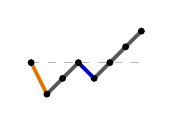
\begin{tikzpicture}[x=0.2cm,y=0.2cm,baseline={([yshift=-0.5ex]current bounding box.center)}]
\draw[gray!55,dashed] (0,0) -- (7,0);
\draw[cB,line width=1.3pt,line cap=round] (0,0) -- (1,-2);
\draw[gray!70!black,line width=1.3pt,line cap=round] (1,-2) -- (2,-1);
\draw[gray!70!black,line width=1.3pt,line cap=round] (2,-1) -- (3,0);
\draw[cA,line width=1.3pt,line cap=round] (3,0) -- (4,-1);
\draw[gray!70!black,line width=1.3pt,line cap=round] (4,-1) -- (5,0);
\draw[gray!70!black,line width=1.3pt,line cap=round] (5,0) -- (6,1);
\draw[gray!70!black,line width=1.3pt,line cap=round] (6,1) -- (7,2);
\fill (0,0) circle (1.25pt);
\fill (1,-2) circle (1.25pt);
\fill (2,-1) circle (1.25pt);
\fill (3,0) circle (1.25pt);
\fill (4,-1) circle (1.25pt);
\fill (5,0) circle (1.25pt);
\fill (6,1) circle (1.25pt);
\fill (7,2) circle (1.25pt);
\end{tikzpicture} & \textcolor{cBad}{$\times$}\\[2pt]\bottomrule\end{tabular}}

\newcommand{\RanAlpha}{%
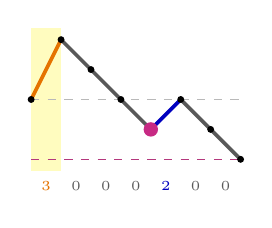
\begin{tikzpicture}[x=0.38cm,y=0.38cm,baseline={([yshift=-0.5ex]current bounding box.center)}]
\fill[yellow!25] (0,-2.4) rectangle (1,2.4);
\draw[gray!55,dashed] (0,0) -- (7,0);
\draw[magenta!70!black,dashed] (0,-2) -- (7,-2);
\draw[cB,line width=1.3pt,line cap=round] (0,0) -- (1,2);
\draw[gray!70!black,line width=1.3pt,line cap=round] (1,2) -- (2,1);
\draw[gray!70!black,line width=1.3pt,line cap=round] (2,1) -- (3,0);
\draw[gray!70!black,line width=1.3pt,line cap=round] (3,0) -- (4,-1);
\draw[cA,line width=1.3pt,line cap=round] (4,-1) -- (5,0);
\draw[gray!70!black,line width=1.3pt,line cap=round] (5,0) -- (6,-1);
\draw[gray!70!black,line width=1.3pt,line cap=round] (6,-1) -- (7,-2);
\fill (0,0) circle (1.25pt);
\fill (1,2) circle (1.25pt);
\fill (2,1) circle (1.25pt);
\fill (3,0) circle (1.25pt);
\fill (4,-1) circle (1.25pt);
\fill (5,0) circle (1.25pt);
\fill (6,-1) circle (1.25pt);
\fill (7,-2) circle (1.25pt);
\fill[magenta!80!black] (4,-1) circle (2.6pt);
\node[font=\tiny,cB] at (0.5,-2.9) {3};
\node[font=\tiny,gray!70!black] at (1.5,-2.9) {0};
\node[font=\tiny,gray!70!black] at (2.5,-2.9) {0};
\node[font=\tiny,gray!70!black] at (3.5,-2.9) {0};
\node[font=\tiny,cA] at (4.5,-2.9) {2};
\node[font=\tiny,gray!70!black] at (5.5,-2.9) {0};
\node[font=\tiny,gray!70!black] at (6.5,-2.9) {0};
\end{tikzpicture}\qquad\begin{tabular}{l}$\sigma_1=\sigma g_{5}=\textcolor{cB}{3}\,\textcolor{gray!70!black}{0}\,\textcolor{gray!70!black}{0}\,\textcolor{gray!70!black}{0}\,\textcolor{cA}{2}\,\textcolor{gray!70!black}{0}\,\textcolor{gray!70!black}{0}$\\[3pt]$\alpha_1=\textcolor{cB}{3}\,\textcolor{gray!70!black}{0}\,\textcolor{gray!70!black}{0}\,\textcolor{gray!70!black}{0},\quad \alpha_2=\textcolor{cA}{2}\,\textcolor{gray!70!black}{0}\,\textcolor{gray!70!black}{0}$\\[3pt]$\sigma_2=\alpha_2\alpha_1=\textcolor{cA}{2}\,\textcolor{gray!70!black}{0}\,\textcolor{gray!70!black}{0}\,\textcolor{cB}{3}\,\textcolor{gray!70!black}{0}\,\textcolor{gray!70!black}{0}\,\textcolor{gray!70!black}{0}=\sigma g_{2}$\end{tabular}}

\newcommand{\RanTwoViews}{%
\begin{tabular}{c}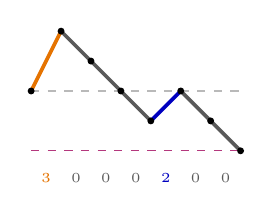
\begin{tikzpicture}[x=0.38cm,y=0.38cm,baseline={([yshift=-0.5ex]current bounding box.center)}]
\draw[gray!55,dashed] (0,0) -- (7,0);
\draw[magenta!70!black,dashed] (0,-2) -- (7,-2);
\draw[cB,line width=1.3pt,line cap=round] (0,0) -- (1,2);
\draw[gray!70!black,line width=1.3pt,line cap=round] (1,2) -- (2,1);
\draw[gray!70!black,line width=1.3pt,line cap=round] (2,1) -- (3,0);
\draw[gray!70!black,line width=1.3pt,line cap=round] (3,0) -- (4,-1);
\draw[cA,line width=1.3pt,line cap=round] (4,-1) -- (5,0);
\draw[gray!70!black,line width=1.3pt,line cap=round] (5,0) -- (6,-1);
\draw[gray!70!black,line width=1.3pt,line cap=round] (6,-1) -- (7,-2);
\fill (0,0) circle (1.25pt);
\fill (1,2) circle (1.25pt);
\fill (2,1) circle (1.25pt);
\fill (3,0) circle (1.25pt);
\fill (4,-1) circle (1.25pt);
\fill (5,0) circle (1.25pt);
\fill (6,-1) circle (1.25pt);
\fill (7,-2) circle (1.25pt);
\node[font=\tiny,cB] at (0.5,-2.9) {3};
\node[font=\tiny,gray!70!black] at (1.5,-2.9) {0};
\node[font=\tiny,gray!70!black] at (2.5,-2.9) {0};
\node[font=\tiny,gray!70!black] at (3.5,-2.9) {0};
\node[font=\tiny,cA] at (4.5,-2.9) {2};
\node[font=\tiny,gray!70!black] at (5.5,-2.9) {0};
\node[font=\tiny,gray!70!black] at (6.5,-2.9) {0};
\end{tikzpicture}\\[2pt]{\small Raney：秩路徑（由左往右讀 $\textcolor{cB}{3}\,\textcolor{gray!70!black}{0}\,\textcolor{gray!70!black}{0}\,\textcolor{gray!70!black}{0}\,\textcolor{cA}{2}\,\textcolor{gray!70!black}{0}\,\textcolor{gray!70!black}{0}$）}\end{tabular}\quad\begin{tabular}{c}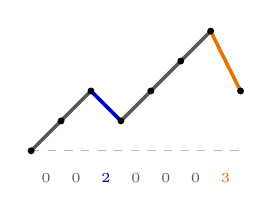
\begin{tikzpicture}[x=0.38cm,y=0.38cm,baseline={([yshift=-0.5ex]current bounding box.center)}]
\draw[gray!55,dashed] (0,0) -- (7,0);
\draw[gray!70!black,line width=1.3pt,line cap=round] (0,0) -- (1,1);
\draw[gray!70!black,line width=1.3pt,line cap=round] (1,1) -- (2,2);
\draw[cA,line width=1.3pt,line cap=round] (2,2) -- (3,1);
\draw[gray!70!black,line width=1.3pt,line cap=round] (3,1) -- (4,2);
\draw[gray!70!black,line width=1.3pt,line cap=round] (4,2) -- (5,3);
\draw[gray!70!black,line width=1.3pt,line cap=round] (5,3) -- (6,4);
\draw[cB,line width=1.3pt,line cap=round] (6,4) -- (7,2);
\fill (0,0) circle (1.25pt);
\fill (1,1) circle (1.25pt);
\fill (2,2) circle (1.25pt);
\fill (3,1) circle (1.25pt);
\fill (4,2) circle (1.25pt);
\fill (5,3) circle (1.25pt);
\fill (6,4) circle (1.25pt);
\fill (7,2) circle (1.25pt);
\node[font=\tiny,gray!70!black] at (0.5,-0.9) {0};
\node[font=\tiny,gray!70!black] at (1.5,-0.9) {0};
\node[font=\tiny,cA] at (2.5,-0.9) {2};
\node[font=\tiny,gray!70!black] at (3.5,-0.9) {0};
\node[font=\tiny,gray!70!black] at (4.5,-0.9) {0};
\node[font=\tiny,gray!70!black] at (5.5,-0.9) {0};
\node[font=\tiny,cB] at (6.5,-0.9) {3};
\end{tikzpicture}\\[2pt]{\small Chu 講義：好路徑（由右往左讀，每步 $1-j$）}\end{tabular}\quad\begin{tabular}{c}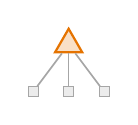
\begin{tikzpicture}[x=0.45cm,y=0.6cm,baseline=(n0.base)]
\node[regular polygon,regular polygon sides=3,draw=cB,fill=cB!22,line width=0.8pt,inner sep=2.0pt] (n0) at (1.000,0) {};
\node[rectangle,draw=gray!70,fill=gray!15,inner sep=1.8pt] (n1) at (0.000,-1) {};
\node[rectangle,draw=gray!70,fill=gray!15,inner sep=1.8pt] (n2) at (1.000,-1) {};
\node[rectangle,draw=gray!70,fill=gray!15,inner sep=1.8pt] (n3) at (2.000,-1) {};
\draw[gray!70,line width=0.6pt] (n0) -- (n1);
\draw[gray!70,line width=0.6pt] (n0) -- (n2);
\draw[gray!70,line width=0.6pt] (n0) -- (n3);
\end{tikzpicture}\hspace{0.90cm}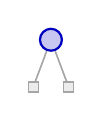
\begin{tikzpicture}[x=0.45cm,y=0.6cm,baseline=(n0.base)]
\node[circle,draw=cA,fill=cA!22,line width=0.8pt,inner sep=2.8pt] (n0) at (0.500,0) {};
\node[rectangle,draw=gray!70,fill=gray!15,inner sep=1.8pt] (n1) at (0.000,-1) {};
\node[rectangle,draw=gray!70,fill=gray!15,inner sep=1.8pt] (n2) at (1.000,-1) {};
\draw[gray!70,line width=0.6pt] (n0) -- (n1);
\draw[gray!70,line width=0.6pt] (n0) -- (n2);
\end{tikzpicture}\\[2pt]{\small 對應的森林（2 棵樹）}\end{tabular}}

\newcommand{\RanThmTwoThree}{%
$\textcolor{cA}{2}\,\textcolor{gray!70!black}{0}\,\textcolor{gray!70!black}{0}\,\textcolor{cB}{3}\,\textcolor{gray!70!black}{0}\,\textcolor{gray!70!black}{0}\,\textcolor{gray!70!black}{0}\ =\ \underbrace{\textcolor{cA}{2}\,\textcolor{gray!70!black}{0}\,\textcolor{gray!70!black}{0}}_{\text{1 字列}}\ \underbrace{\textcolor{cB}{3}\,\textcolor{gray!70!black}{0}\,\textcolor{gray!70!black}{0}\,\textcolor{gray!70!black}{0}}_{\text{1 字列}}$\qquad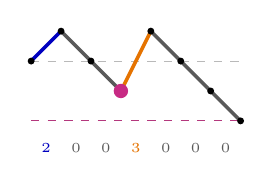
\begin{tikzpicture}[x=0.38cm,y=0.38cm,baseline={([yshift=-0.5ex]current bounding box.center)}]
\draw[gray!55,dashed] (0,0) -- (7,0);
\draw[magenta!70!black,dashed] (0,-2) -- (7,-2);
\draw[cA,line width=1.3pt,line cap=round] (0,0) -- (1,1);
\draw[gray!70!black,line width=1.3pt,line cap=round] (1,1) -- (2,0);
\draw[gray!70!black,line width=1.3pt,line cap=round] (2,0) -- (3,-1);
\draw[cB,line width=1.3pt,line cap=round] (3,-1) -- (4,1);
\draw[gray!70!black,line width=1.3pt,line cap=round] (4,1) -- (5,0);
\draw[gray!70!black,line width=1.3pt,line cap=round] (5,0) -- (6,-1);
\draw[gray!70!black,line width=1.3pt,line cap=round] (6,-1) -- (7,-2);
\fill (0,0) circle (1.25pt);
\fill (1,1) circle (1.25pt);
\fill (2,0) circle (1.25pt);
\fill (3,-1) circle (1.25pt);
\fill (4,1) circle (1.25pt);
\fill (5,0) circle (1.25pt);
\fill (6,-1) circle (1.25pt);
\fill (7,-2) circle (1.25pt);
\fill[magenta!80!black] (3,-1) circle (2.6pt);
\node[font=\tiny,cA] at (0.5,-2.9) {2};
\node[font=\tiny,gray!70!black] at (1.5,-2.9) {0};
\node[font=\tiny,gray!70!black] at (2.5,-2.9) {0};
\node[font=\tiny,cB] at (3.5,-2.9) {3};
\node[font=\tiny,gray!70!black] at (4.5,-2.9) {0};
\node[font=\tiny,gray!70!black] at (5.5,-2.9) {0};
\node[font=\tiny,gray!70!black] at (6.5,-2.9) {0};
\end{tikzpicture}}

\newcommand{\RanMotzkin}{%
\begin{tabular}{cccc}\begin{tabular}{c}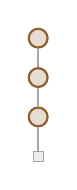
\begin{tikzpicture}[x=0.45cm,y=0.5cm,baseline=(n0.base)]
\node[circle,draw=cU,fill=cU!22,line width=0.8pt,inner sep=2.4pt] (n0) at (0.000,0) {};
\node[circle,draw=cU,fill=cU!22,line width=0.8pt,inner sep=2.4pt] (n1) at (0.000,-1) {};
\node[circle,draw=cU,fill=cU!22,line width=0.8pt,inner sep=2.4pt] (n2) at (0.000,-2) {};
\node[rectangle,draw=gray!70,fill=gray!15,inner sep=1.8pt] (n3) at (0.000,-3) {};
\draw[gray!70,line width=0.6pt] (n2) -- (n3);
\draw[gray!70,line width=0.6pt] (n1) -- (n2);
\draw[gray!70,line width=0.6pt] (n0) -- (n1);
\end{tikzpicture}\\[2pt]$\textcolor{cU}{1}\,\textcolor{cU}{1}\,\textcolor{cU}{1}\,\textcolor{gray!70!black}{0}$\end{tabular} & \begin{tabular}{c}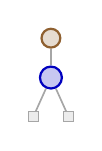
\begin{tikzpicture}[x=0.45cm,y=0.5cm,baseline=(n0.base)]
\node[circle,draw=cU,fill=cU!22,line width=0.8pt,inner sep=2.4pt] (n0) at (0.500,0) {};
\node[circle,draw=cA,fill=cA!22,line width=0.8pt,inner sep=2.8pt] (n1) at (0.500,-1) {};
\node[rectangle,draw=gray!70,fill=gray!15,inner sep=1.8pt] (n2) at (0.000,-2) {};
\node[rectangle,draw=gray!70,fill=gray!15,inner sep=1.8pt] (n3) at (1.000,-2) {};
\draw[gray!70,line width=0.6pt] (n1) -- (n2);
\draw[gray!70,line width=0.6pt] (n1) -- (n3);
\draw[gray!70,line width=0.6pt] (n0) -- (n1);
\end{tikzpicture}\\[2pt]$\textcolor{cU}{1}\,\textcolor{cA}{2}\,\textcolor{gray!70!black}{0}\,\textcolor{gray!70!black}{0}$\end{tabular} & \begin{tabular}{c}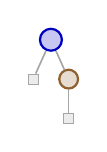
\begin{tikzpicture}[x=0.45cm,y=0.5cm,baseline=(n0.base)]
\node[circle,draw=cA,fill=cA!22,line width=0.8pt,inner sep=2.8pt] (n0) at (0.500,0) {};
\node[rectangle,draw=gray!70,fill=gray!15,inner sep=1.8pt] (n1) at (0.000,-1) {};
\node[circle,draw=cU,fill=cU!22,line width=0.8pt,inner sep=2.4pt] (n2) at (1.000,-1) {};
\node[rectangle,draw=gray!70,fill=gray!15,inner sep=1.8pt] (n3) at (1.000,-2) {};
\draw[gray!70,line width=0.6pt] (n2) -- (n3);
\draw[gray!70,line width=0.6pt] (n0) -- (n1);
\draw[gray!70,line width=0.6pt] (n0) -- (n2);
\end{tikzpicture}\\[2pt]$\textcolor{cA}{2}\,\textcolor{gray!70!black}{0}\,\textcolor{cU}{1}\,\textcolor{gray!70!black}{0}$\end{tabular} & \begin{tabular}{c}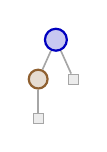
\begin{tikzpicture}[x=0.45cm,y=0.5cm,baseline=(n0.base)]
\node[circle,draw=cA,fill=cA!22,line width=0.8pt,inner sep=2.8pt] (n0) at (0.500,0) {};
\node[circle,draw=cU,fill=cU!22,line width=0.8pt,inner sep=2.4pt] (n1) at (0.000,-1) {};
\node[rectangle,draw=gray!70,fill=gray!15,inner sep=1.8pt] (n2) at (0.000,-2) {};
\node[rectangle,draw=gray!70,fill=gray!15,inner sep=1.8pt] (n3) at (1.000,-1) {};
\draw[gray!70,line width=0.6pt] (n1) -- (n2);
\draw[gray!70,line width=0.6pt] (n0) -- (n1);
\draw[gray!70,line width=0.6pt] (n0) -- (n3);
\end{tikzpicture}\\[2pt]$\textcolor{cA}{2}\,\textcolor{cU}{1}\,\textcolor{gray!70!black}{0}\,\textcolor{gray!70!black}{0}$\end{tabular}\end{tabular}}

\newcommand{\RanGesselCodes}{%
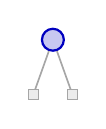
\begin{tikzpicture}[x=0.5cm,y=0.7cm,baseline=(n0.base)]
\node[circle,draw=cA,fill=cA!22,line width=0.8pt,inner sep=2.8pt] (n0) at (0.500,0) {};
\node[rectangle,draw=gray!70,fill=gray!15,inner sep=1.8pt] (n1) at (0.000,-1) {};
\node[rectangle,draw=gray!70,fill=gray!15,inner sep=1.8pt] (n2) at (1.000,-1) {};
\draw[gray!70,line width=0.6pt] (n0) -- (n1);
\draw[gray!70,line width=0.6pt] (n0) -- (n2);
\end{tikzpicture}\hspace{0.90cm}
\begin{tikzpicture}[x=0.5cm,y=0.7cm,baseline=(n0.base)]
\node[circle,draw=cU,fill=cU!22,line width=0.8pt,inner sep=2.4pt] (n0) at (0.000,0) {};
\node[rectangle,draw=gray!70,fill=gray!15,inner sep=1.8pt] (n1) at (0.000,-1) {};
\draw[gray!70,line width=0.6pt] (n0) -- (n1);
\end{tikzpicture}\qquad\begin{tabular}{@{}ll@{}}
Raney 的前序碼（2 字列） & $\textcolor{cA}{2}\,\textcolor{gray!70!black}{0}\,\textcolor{gray!70!black}{0}\,\textcolor{cU}{1}\,\textcolor{gray!70!black}{0}$\\
Gessel 的 suffix code $c(T_1)c(T_2)$ & $\textcolor{gray!70!black}{0}\,\textcolor{gray!70!black}{0}\,\textcolor{cA}{2}\,\textcolor{gray!70!black}{0}\,\textcolor{cU}{1}$\\
reduced code（每項減 1） & $-1\ -1\ 1\ -1\ 0$\\
reduced code 的部分和 & $-1,\ -2,\ -1,\ -2,\ -2$（全部 $<0$，總和 $-2$）\\
Chu 講義的路徑高度（取負號） & $1,\ 2,\ 1,\ 2,\ 2$\\
\end{tabular}}

\newcommand{\RanHexagon}{%

\begin{tikzpicture}[scale=0.55,baseline=-0.5ex]\foreach \i in {0,...,5}{\coordinate (h\i) at ({90-60*\i}:1);}\draw[cC,line width=1pt,fill=cC!12] (h0)--(h1)--(h2)--(h3)--(h4)--(h5)--cycle;\draw[cC,line width=1.2pt] (h0)--(h3);\foreach \i in {0,...,5}{\fill (h\i) circle (1.4pt);}\end{tikzpicture}\quad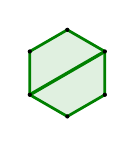
\begin{tikzpicture}[scale=0.55,baseline=-0.5ex]\foreach \i in {0,...,5}{\coordinate (h\i) at ({90-60*\i}:1);}\draw[cC,line width=1pt,fill=cC!12] (h0)--(h1)--(h2)--(h3)--(h4)--(h5)--cycle;\draw[cC,line width=1.2pt] (h1)--(h4);\foreach \i in {0,...,5}{\fill (h\i) circle (1.4pt);}\end{tikzpicture}\quad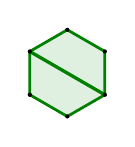
\begin{tikzpicture}[scale=0.55,baseline=-0.5ex]\foreach \i in {0,...,5}{\coordinate (h\i) at ({90-60*\i}:1);}\draw[cC,line width=1pt,fill=cC!12] (h0)--(h1)--(h2)--(h3)--(h4)--(h5)--cycle;\draw[cC,line width=1.2pt] (h2)--(h5);\foreach \i in {0,...,5}{\fill (h\i) circle (1.4pt);}\end{tikzpicture}}

\newcommand{\RanLTable}{%
\setlength{\tabcolsep}{3.6pt}\begin{tabular}{@{}lccccccl@{}}\toprule
組成 $(n;a_1,a_2,\ldots)$ & $a_0$ & $m$ & $M(a_0,a_1,\ldots)$ & $\frac{n}{m}M$ & 暴力 & Chu：$t$、$\vn$、$\vv$ & 白話\\\midrule
$(1;\,0,3)$ & 4 & 7 & 35 & 5 & 5 & $1$、$(3)$、$(2)$ & Cayley：4 個因子的乘積\\
$(1;\,0,0,3)$ & 7 & 10 & 120 & 12 & 12 & $1$、$(3)$、$(3)$ & 3 個三元運算\\
$(1;\,1,1)$ & 2 & 4 & 12 & 3 & 3 & $1$、$(1,1)$、$(1,2)$ & 一元＋二元各 1\\
$(1;\,0,1,1)$ & 4 & 6 & 30 & 5 & 5 & $1$、$(1,1)$、$(2,3)$ & Chu 原文 Fig.~1\\
$(2;\,0,1,1)$ & 5 & 7 & 42 & 12 & 12 & $2$、$(1,1)$、$(2,3)$ & 同上，2 字列\\
$(1;\,0,2,1)$ & 5 & 8 & 168 & 21 & 21 & $1$、$(2,1)$、$(2,3)$ & 2 弦 1 三角形\\
$(1;\,0,1,2)$ & 6 & 9 & 252 & 28 & 28 & $1$、$(1,2)$、$(2,3)$ & 1 弦 2 三角形\\
$(1;\,0,2,2)$ & 7 & 11 & 1980 & 180 & 180 & $1$、$(2,2)$、$(2,3)$ & 2 弦 2 三角形\\
$(1;\,0,1,1,1)$ & 7 & 10 & 720 & 72 & 72 & $1$、$(1,1,1)$、$(2,3,4)$ & 弦、三角形、四邊形各 1\\
$(1;\,2,2)$ & 3 & 7 & 210 & 30 & 30 & $1$、$(2,2)$、$(1,2)$ & 2 個單點、2 條弦\\
$(3;\,0,2)$ & 5 & 7 & 21 & 9 & 9 & $3$、$(2)$、$(2)$ & 3 棵二元樹，共 2 個內部節點\\
\bottomrule\end{tabular}}

\newcommand{\RanThmTwoThreeTable}{%
\begin{tabular}{cccc}\toprule $b=(b_1,b_2,b_3)$ & $L(1;b)$ & $L(1;a-b)$ & 乘積\\\midrule
$(0,0,0)$ & 1 & 5 & 5\\
$(0,1,0)$ & 1 & 1 & 1\\
$(0,0,1)$ & 1 & 1 & 1\\
$(0,1,1)$ & 5 & 1 & 5\\
\midrule\multicolumn{3}{r}{合計} & $12=L(2;0,1,1)$\\\bottomrule\end{tabular}}

\newcommand{\RanLstarTable}{%
\begin{tabular}{@{}clccc@{}}\toprule 權重 $\sum ip_i$ & 單項式 $E^*_{\bar p}$ & $L(1;\bar p)$ & $L(2;\bar p)$ & 例：$n=1$ 的字\\\midrule
0 & $E_0^*$ & 1 & 1 & $\textcolor{gray!70!black}{0}$\\
1 & $E_1^*$ & 1 & 2 & $\textcolor{cU}{1}\,\textcolor{gray!70!black}{0}$\\
2 & $(E_1^*)^2$ & 1 & 3 & $\textcolor{cU}{1}\,\textcolor{cU}{1}\,\textcolor{gray!70!black}{0}$\\
2 & $E_2^*$ & 1 & 2 & $\textcolor{cA}{2}\,\textcolor{gray!70!black}{0}\,\textcolor{gray!70!black}{0}$\\
3 & $(E_1^*)^3$ & 1 & 4 & $\textcolor{cU}{1}\,\textcolor{cU}{1}\,\textcolor{cU}{1}\,\textcolor{gray!70!black}{0}$\\
3 & $E_1^*\,E_2^*$ & 3 & 8 & $\textcolor{cU}{1}\,\textcolor{cA}{2}\,\textcolor{gray!70!black}{0}\,\textcolor{gray!70!black}{0}$、…（共 3 個）\\
3 & $E_3^*$ & 1 & 2 & $\textcolor{cB}{3}\,\textcolor{gray!70!black}{0}\,\textcolor{gray!70!black}{0}\,\textcolor{gray!70!black}{0}$\\
4 & $(E_1^*)^4$ & 1 & 5 & $\textcolor{cU}{1}\,\textcolor{cU}{1}\,\textcolor{cU}{1}\,\textcolor{cU}{1}\,\textcolor{gray!70!black}{0}$\\
4 & $(E_1^*)^2\,E_2^*$ & 6 & 20 & $\textcolor{cU}{1}\,\textcolor{cU}{1}\,\textcolor{cA}{2}\,\textcolor{gray!70!black}{0}\,\textcolor{gray!70!black}{0}$、…（共 6 個）\\
4 & $E_1^*\,E_3^*$ & 4 & 10 & $\textcolor{cU}{1}\,\textcolor{cB}{3}\,\textcolor{gray!70!black}{0}\,\textcolor{gray!70!black}{0}\,\textcolor{gray!70!black}{0}$、…（共 4 個）\\
4 & $(E_2^*)^2$ & 2 & 5 & $\textcolor{cA}{2}\,\textcolor{gray!70!black}{0}\,\textcolor{cA}{2}\,\textcolor{gray!70!black}{0}\,\textcolor{gray!70!black}{0}$、…（共 2 個）\\
4 & $E_4^*$ & 1 & 2 & $\textcolor{cC}{4}\,\textcolor{gray!70!black}{0}\,\textcolor{gray!70!black}{0}\,\textcolor{gray!70!black}{0}\,\textcolor{gray!70!black}{0}$\\
\bottomrule\end{tabular}}

\newcommand{\RanTrinomialTable}{%
\begin{tabular}{@{}c|rrrrrrr@{}}$n\backslash k$ & 0 & 1 & 2 & 3 & 4 & 5 & 6\\\hline
2 & 1 & 1 & 2 & 5 & 14 & 42 & 132\\
3 & 1 & 1 & 3 & 12 & 55 & 273 & 1428\\
4 & 1 & 1 & 4 & 22 & 140 & 969 & 7084\\
\end{tabular}}

\newcommand{\RanKellyTable}{%
\begin{tabular}{@{}c|rrrrrrrrrr@{}}$r\backslash n$ & 1 & 2 & 3 & 4 & 5 & 6 & 7 & 8 & 9 & 10\\\hline
1 & 1 & 1 & 2 & 5 & 14 & 42 & 132 & 429 & 1430 & 4862\\
2 & 1 & 0 & 1 & 0 & 3 & 0 & 12 & 0 & 55 & 0\\
3 & 1 & 0 & 0 & 1 & 0 & 0 & 4 & 0 & 0 & 22\\
\end{tabular}}

\newcommand{\RanLagrangeTable}{%
\setlength{\tabcolsep}{3.5pt}\begin{tabular}{@{}lllccccccl@{}}\toprule $\bar z=\sum a_n\bar x^n$ & 方程 (5.3) & & $n=1$ & $n=2$ & $n=3$ & $n=4$ & $n=5$ & $n=6$ & 名稱\\\midrule
$\dfrac{1}{1-x}$ & $w=\dfrac{x}{1-w}$ & 逐次代入 & $1$ & $1$ & $2$ & $5$ & $14$ & $42$ & $C_{n-1}$（卡塔蘭）\\
 & & 式 (5.5) & $1$ & $1$ & $2$ & $5$ & $14$ & $42$ & \\[2pt]
$(1+x)^2$ & $w=x(1+w)^2$ & 逐次代入 & $1$ & $2$ & $5$ & $14$ & $42$ & $132$ & $C_n$\\
 & & 式 (5.5) & $1$ & $2$ & $5$ & $14$ & $42$ & $132$ & \\[2pt]
$1+x+x^2$ & $w=x(1+w+w^2)$ & 逐次代入 & $1$ & $1$ & $2$ & $4$ & $9$ & $21$ & Motzkin 數 $M_{n-1}$\\
 & & 式 (5.5) & $1$ & $1$ & $2$ & $4$ & $9$ & $21$ & \\[2pt]
$e^x$ & $w=xe^{w}$ & 逐次代入 & $1$ & $1$ & $\tfrac{3}{2}$ & $\tfrac{8}{3}$ & $\tfrac{125}{24}$ & $\tfrac{54}{5}$ & $n^{n-1}/n!$（樹函數）\\
 & & 式 (5.5) & $1$ & $1$ & $\tfrac{3}{2}$ & $\tfrac{8}{3}$ & $\tfrac{125}{24}$ & $\tfrac{54}{5}$ & \\[2pt]
$2+3x+x^3$ & $w=x(2+3w+w^3)$ & 逐次代入 & $2$ & $6$ & $18$ & $62$ & $258$ & $1206$ & $a_0\ne1$ 的例子\\
 & & 式 (5.5) & $2$ & $6$ & $18$ & $62$ & $258$ & $1206$ & \\[2pt]
\bottomrule\end{tabular}}

\newcommand{\RanBallotTable}{%
\begin{tabular}{@{}c|rrrrrr@{}}$m\backslash n$ & 0 & 1 & 2 & 3 & 4 & 5\\\hline
1 & 1 & 1 & 2 & 5 & 14 & 42\\
2 & 1 & 2 & 5 & 14 & 42 & 132\\
3 & 1 & 3 & 9 & 28 & 90 & 297\\
\end{tabular}}

\newcommand{\RanNotWord}{%
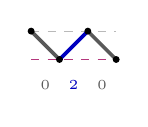
\begin{tikzpicture}[x=0.36cm,y=0.36cm,baseline={([yshift=-0.5ex]current bounding box.center)}]
\draw[gray!55,dashed] (0,0) -- (3,0);
\draw[magenta!70!black,dashed] (0,-1) -- (3,-1);
\draw[gray!70!black,line width=1.3pt,line cap=round] (0,0) -- (1,-1);
\draw[cA,line width=1.3pt,line cap=round] (1,-1) -- (2,0);
\draw[gray!70!black,line width=1.3pt,line cap=round] (2,0) -- (3,-1);
\fill (0,0) circle (1.25pt);
\fill (1,-1) circle (1.25pt);
\fill (2,0) circle (1.25pt);
\fill (3,-1) circle (1.25pt);
\node[font=\tiny,gray!70!black] at (0.5,-1.9) {0};
\node[font=\tiny,cA] at (1.5,-1.9) {2};
\node[font=\tiny,gray!70!black] at (2.5,-1.9) {0};
\end{tikzpicture}}

\newcommand{\RanWalkPlusOne}{%
\begin{tikzpicture}[x=0.3cm,y=0.3cm,baseline={([yshift=-0.5ex]current bounding box.center)}]
\draw[gray!55,dashed] (0,0) -- (5,0);
\draw[magenta!70!black,dashed] (0,-1) -- (5,-1);
\draw[cA,line width=1.3pt,line cap=round] (0,0) -- (1,1);
\draw[cA,line width=1.3pt,line cap=round] (1,1) -- (2,2);
\draw[gray!70!black,line width=1.3pt,line cap=round] (2,2) -- (3,1);
\draw[gray!70!black,line width=1.3pt,line cap=round] (3,1) -- (4,0);
\draw[gray!70!black,line width=1.3pt,line cap=round] (4,0) -- (5,-1);
\fill (0,0) circle (1.25pt);
\fill (1,1) circle (1.25pt);
\fill (2,2) circle (1.25pt);
\fill (3,1) circle (1.25pt);
\fill (4,0) circle (1.25pt);
\fill (5,-1) circle (1.25pt);
\node[font=\tiny,cA] at (0.5,-1.9) {2};
\node[font=\tiny,cA] at (1.5,-1.9) {2};
\node[font=\tiny,gray!70!black] at (2.5,-1.9) {0};
\node[font=\tiny,gray!70!black] at (3.5,-1.9) {0};
\node[font=\tiny,gray!70!black] at (4.5,-1.9) {0};
\end{tikzpicture}}

\newcommand{\RanWalkPlusTwo}{%
\begin{tikzpicture}[x=0.3cm,y=0.3cm,baseline={([yshift=-0.5ex]current bounding box.center)}]
\draw[gray!55,dashed] (0,0) -- (5,0);
\draw[magenta!70!black,dashed] (0,-1) -- (5,-1);
\draw[cA,line width=1.3pt,line cap=round] (0,0) -- (1,1);
\draw[gray!70!black,line width=1.3pt,line cap=round] (1,1) -- (2,0);
\draw[cA,line width=1.3pt,line cap=round] (2,0) -- (3,1);
\draw[gray!70!black,line width=1.3pt,line cap=round] (3,1) -- (4,0);
\draw[gray!70!black,line width=1.3pt,line cap=round] (4,0) -- (5,-1);
\fill (0,0) circle (1.25pt);
\fill (1,1) circle (1.25pt);
\fill (2,0) circle (1.25pt);
\fill (3,1) circle (1.25pt);
\fill (4,0) circle (1.25pt);
\fill (5,-1) circle (1.25pt);
\node[font=\tiny,cA] at (0.5,-1.9) {2};
\node[font=\tiny,gray!70!black] at (1.5,-1.9) {0};
\node[font=\tiny,cA] at (2.5,-1.9) {2};
\node[font=\tiny,gray!70!black] at (3.5,-1.9) {0};
\node[font=\tiny,gray!70!black] at (4.5,-1.9) {0};
\end{tikzpicture}}

\newcommand{\RanCycThree}{%
\begin{tabular}{c c c c}\toprule $k$ & $\sigma g_k$ & 秩路徑 & $n$ 字列？\\\midrule
0 & $\textcolor{cA}{2}\,\textcolor{gray!70!black}{0}\,\textcolor{gray!70!black}{0}\,\textcolor{cA}{2}\,\textcolor{gray!70!black}{0}\,\textcolor{gray!70!black}{0}$ & \begin{tikzpicture}[x=0.2cm,y=0.2cm,baseline={([yshift=-0.5ex]current bounding box.center)}]
\draw[gray!55,dashed] (0,0) -- (6,0);
\draw[magenta!70!black,dashed] (0,-2) -- (6,-2);
\draw[cA,line width=1.3pt,line cap=round] (0,0) -- (1,1);
\draw[gray!70!black,line width=1.3pt,line cap=round] (1,1) -- (2,0);
\draw[gray!70!black,line width=1.3pt,line cap=round] (2,0) -- (3,-1);
\draw[cA,line width=1.3pt,line cap=round] (3,-1) -- (4,0);
\draw[gray!70!black,line width=1.3pt,line cap=round] (4,0) -- (5,-1);
\draw[gray!70!black,line width=1.3pt,line cap=round] (5,-1) -- (6,-2);
\fill (0,0) circle (1.25pt);
\fill (1,1) circle (1.25pt);
\fill (2,0) circle (1.25pt);
\fill (3,-1) circle (1.25pt);
\fill (4,0) circle (1.25pt);
\fill (5,-1) circle (1.25pt);
\fill (6,-2) circle (1.25pt);
\end{tikzpicture} & \textcolor{green!50!black}{\checkmark}\\[2pt]
1 & $\textcolor{gray!70!black}{0}\,\textcolor{gray!70!black}{0}\,\textcolor{cA}{2}\,\textcolor{gray!70!black}{0}\,\textcolor{gray!70!black}{0}\,\textcolor{cA}{2}$ & \begin{tikzpicture}[x=0.2cm,y=0.2cm,baseline={([yshift=-0.5ex]current bounding box.center)}]
\draw[gray!55,dashed] (0,0) -- (6,0);
\draw[magenta!70!black,dashed] (0,-2) -- (6,-2);
\draw[gray!70!black,line width=1.3pt,line cap=round] (0,0) -- (1,-1);
\draw[gray!70!black,line width=1.3pt,line cap=round] (1,-1) -- (2,-2);
\draw[cA,line width=1.3pt,line cap=round] (2,-2) -- (3,-1);
\draw[gray!70!black,line width=1.3pt,line cap=round] (3,-1) -- (4,-2);
\draw[gray!70!black,line width=1.3pt,line cap=round] (4,-2) -- (5,-3);
\draw[cA,line width=1.3pt,line cap=round] (5,-3) -- (6,-2);
\fill (0,0) circle (1.25pt);
\fill (1,-1) circle (1.25pt);
\fill (2,-2) circle (1.25pt);
\fill (3,-1) circle (1.25pt);
\fill (4,-2) circle (1.25pt);
\fill (5,-3) circle (1.25pt);
\fill (6,-2) circle (1.25pt);
\end{tikzpicture} & \textcolor{cBad}{$\times$}\\[2pt]
2 & $\textcolor{gray!70!black}{0}\,\textcolor{cA}{2}\,\textcolor{gray!70!black}{0}\,\textcolor{gray!70!black}{0}\,\textcolor{cA}{2}\,\textcolor{gray!70!black}{0}$ & \begin{tikzpicture}[x=0.2cm,y=0.2cm,baseline={([yshift=-0.5ex]current bounding box.center)}]
\draw[gray!55,dashed] (0,0) -- (6,0);
\draw[magenta!70!black,dashed] (0,-2) -- (6,-2);
\draw[gray!70!black,line width=1.3pt,line cap=round] (0,0) -- (1,-1);
\draw[cA,line width=1.3pt,line cap=round] (1,-1) -- (2,0);
\draw[gray!70!black,line width=1.3pt,line cap=round] (2,0) -- (3,-1);
\draw[gray!70!black,line width=1.3pt,line cap=round] (3,-1) -- (4,-2);
\draw[cA,line width=1.3pt,line cap=round] (4,-2) -- (5,-1);
\draw[gray!70!black,line width=1.3pt,line cap=round] (5,-1) -- (6,-2);
\fill (0,0) circle (1.25pt);
\fill (1,-1) circle (1.25pt);
\fill (2,0) circle (1.25pt);
\fill (3,-1) circle (1.25pt);
\fill (4,-2) circle (1.25pt);
\fill (5,-1) circle (1.25pt);
\fill (6,-2) circle (1.25pt);
\end{tikzpicture} & \textcolor{cBad}{$\times$}\\[2pt]
3 & $\textcolor{cA}{2}\,\textcolor{gray!70!black}{0}\,\textcolor{gray!70!black}{0}\,\textcolor{cA}{2}\,\textcolor{gray!70!black}{0}\,\textcolor{gray!70!black}{0}$ & \begin{tikzpicture}[x=0.2cm,y=0.2cm,baseline={([yshift=-0.5ex]current bounding box.center)}]
\draw[gray!55,dashed] (0,0) -- (6,0);
\draw[magenta!70!black,dashed] (0,-2) -- (6,-2);
\draw[cA,line width=1.3pt,line cap=round] (0,0) -- (1,1);
\draw[gray!70!black,line width=1.3pt,line cap=round] (1,1) -- (2,0);
\draw[gray!70!black,line width=1.3pt,line cap=round] (2,0) -- (3,-1);
\draw[cA,line width=1.3pt,line cap=round] (3,-1) -- (4,0);
\draw[gray!70!black,line width=1.3pt,line cap=round] (4,0) -- (5,-1);
\draw[gray!70!black,line width=1.3pt,line cap=round] (5,-1) -- (6,-2);
\fill (0,0) circle (1.25pt);
\fill (1,1) circle (1.25pt);
\fill (2,0) circle (1.25pt);
\fill (3,-1) circle (1.25pt);
\fill (4,0) circle (1.25pt);
\fill (5,-1) circle (1.25pt);
\fill (6,-2) circle (1.25pt);
\end{tikzpicture} & \textcolor{green!50!black}{\checkmark}\\[2pt]
4 & $\textcolor{gray!70!black}{0}\,\textcolor{gray!70!black}{0}\,\textcolor{cA}{2}\,\textcolor{gray!70!black}{0}\,\textcolor{gray!70!black}{0}\,\textcolor{cA}{2}$ & \begin{tikzpicture}[x=0.2cm,y=0.2cm,baseline={([yshift=-0.5ex]current bounding box.center)}]
\draw[gray!55,dashed] (0,0) -- (6,0);
\draw[magenta!70!black,dashed] (0,-2) -- (6,-2);
\draw[gray!70!black,line width=1.3pt,line cap=round] (0,0) -- (1,-1);
\draw[gray!70!black,line width=1.3pt,line cap=round] (1,-1) -- (2,-2);
\draw[cA,line width=1.3pt,line cap=round] (2,-2) -- (3,-1);
\draw[gray!70!black,line width=1.3pt,line cap=round] (3,-1) -- (4,-2);
\draw[gray!70!black,line width=1.3pt,line cap=round] (4,-2) -- (5,-3);
\draw[cA,line width=1.3pt,line cap=round] (5,-3) -- (6,-2);
\fill (0,0) circle (1.25pt);
\fill (1,-1) circle (1.25pt);
\fill (2,-2) circle (1.25pt);
\fill (3,-1) circle (1.25pt);
\fill (4,-2) circle (1.25pt);
\fill (5,-3) circle (1.25pt);
\fill (6,-2) circle (1.25pt);
\end{tikzpicture} & \textcolor{cBad}{$\times$}\\[2pt]
5 & $\textcolor{gray!70!black}{0}\,\textcolor{cA}{2}\,\textcolor{gray!70!black}{0}\,\textcolor{gray!70!black}{0}\,\textcolor{cA}{2}\,\textcolor{gray!70!black}{0}$ & \begin{tikzpicture}[x=0.2cm,y=0.2cm,baseline={([yshift=-0.5ex]current bounding box.center)}]
\draw[gray!55,dashed] (0,0) -- (6,0);
\draw[magenta!70!black,dashed] (0,-2) -- (6,-2);
\draw[gray!70!black,line width=1.3pt,line cap=round] (0,0) -- (1,-1);
\draw[cA,line width=1.3pt,line cap=round] (1,-1) -- (2,0);
\draw[gray!70!black,line width=1.3pt,line cap=round] (2,0) -- (3,-1);
\draw[gray!70!black,line width=1.3pt,line cap=round] (3,-1) -- (4,-2);
\draw[cA,line width=1.3pt,line cap=round] (4,-2) -- (5,-1);
\draw[gray!70!black,line width=1.3pt,line cap=round] (5,-1) -- (6,-2);
\fill (0,0) circle (1.25pt);
\fill (1,-1) circle (1.25pt);
\fill (2,0) circle (1.25pt);
\fill (3,-1) circle (1.25pt);
\fill (4,-2) circle (1.25pt);
\fill (5,-1) circle (1.25pt);
\fill (6,-2) circle (1.25pt);
\end{tikzpicture} & \textcolor{cBad}{$\times$}\\[2pt]\bottomrule\end{tabular}}

\newcommand{\RanLadder}{%
\begin{tabular}{@{}>{\raggedright}p{2.3cm}>{\raggedright}p{3.4cm}>{\raggedright}p{3.0cm}cl@{}}\toprule
推廣 & Chu 講義的物件 & Raney 的字 & 個數 & 例子\\\midrule
卡塔蘭 $C_n$ & 只用弦（2 點群組），$t=1$ & 只有 2、0 的字 & $\frac{1}{2n+1}\binom{2n+1}{n}$ & $n=3$：5\\
Fuss--Catalan & 只用 $v$ 點群組，$t=1$ & 只有 $v$、0 的字 & $\frac{1}{(v-1)n+1}\binom{vn}{n}$ & $v=3,\ n=2$：3\\
Chu 的 $\Cv(\vn)$ & $n_i$ 個 $v_i$ 點群組，$t=1$ & 符號 $v_i$ 出現 $n_i$ 次的字 & $\frac{1}{N+1}\binom{N+1}{\vn}$ & 一條弦＋一個三角形：5\\
Chu 的 $A_t(\vn)$ & 同上，固定點 $t$ 個 & $t$ 字列（$t$ 棵樹） & $\frac{t}{N+t}\binom{N+t}{\vn}$ & 同上，$t=2$：12\\
\bottomrule\end{tabular}}

\newcommand{\RanBinaryWords}{%
\begin{tabular}{@{}lll@{}}\toprule 字 & 運算式 & Chu 路徑的高度（倒過來讀，步 $1-a$）\\\midrule
$\textcolor{cA}{2}\,\textcolor{cA}{2}\,\textcolor{cA}{2}\,\textcolor{gray!70!black}{0}\,\textcolor{gray!70!black}{0}\,\textcolor{gray!70!black}{0}\,\textcolor{gray!70!black}{0}$ & $((a+b)+c)+d$ & 1, 2, 3, 4, 3, 2, 1\\
$\textcolor{cA}{2}\,\textcolor{cA}{2}\,\textcolor{gray!70!black}{0}\,\textcolor{cA}{2}\,\textcolor{gray!70!black}{0}\,\textcolor{gray!70!black}{0}\,\textcolor{gray!70!black}{0}$ & $(a+(b+c))+d$ & 1, 2, 3, 2, 3, 2, 1\\
$\textcolor{cA}{2}\,\textcolor{cA}{2}\,\textcolor{gray!70!black}{0}\,\textcolor{gray!70!black}{0}\,\textcolor{cA}{2}\,\textcolor{gray!70!black}{0}\,\textcolor{gray!70!black}{0}$ & $(a+b)+(c+d)$ & 1, 2, 1, 2, 3, 2, 1\\
$\textcolor{cA}{2}\,\textcolor{gray!70!black}{0}\,\textcolor{cA}{2}\,\textcolor{cA}{2}\,\textcolor{gray!70!black}{0}\,\textcolor{gray!70!black}{0}\,\textcolor{gray!70!black}{0}$ & $a+((b+c)+d)$ & 1, 2, 3, 2, 1, 2, 1\\
$\textcolor{cA}{2}\,\textcolor{gray!70!black}{0}\,\textcolor{cA}{2}\,\textcolor{gray!70!black}{0}\,\textcolor{cA}{2}\,\textcolor{gray!70!black}{0}\,\textcolor{gray!70!black}{0}$ & $a+(b+(c+d))$ & 1, 2, 1, 2, 1, 2, 1\\
\bottomrule\end{tabular}}

\newcommand{\RanNeyView}{%
\begin{tikzpicture}[x=0.5cm,y=0.5cm]
\draw[gray!25] (0,0) grid (10,6);
\draw[cTop,dashed] (0,3) -- (12.2,3) node[right,font=\scriptsize] {$S_{10}=3$};
\draw[cLeft,-{Stealth[length=4pt]},line width=0.8pt] (12.2,0) -- (0.18,0);
\draw[cLeft,-{Stealth[length=4pt]},line width=0.8pt] (12.2,1) -- (2.18,1);
\draw[cLeft,-{Stealth[length=4pt]},line width=0.8pt] (12.2,2) -- (5.18,2);
\draw[cA,line width=1.3pt,line join=round] (0,0) -- (1,2) -- (2,1) -- (3,3) -- (4,5) -- (5,2) -- (6,4) -- (7,5) -- (8,6) -- (9,5) -- (10,3);
\fill[cRoot] (0,0) circle (3pt) node[below=2pt,font=\scriptsize,cRoot] {$S_{0}$};
\fill (1,2) circle (1.6pt);
\fill[cRoot] (2,1) circle (3pt) node[below=2pt,font=\scriptsize,cRoot] {$S_{2}$};
\fill (3,3) circle (1.6pt);
\fill (4,5) circle (1.6pt);
\fill[cRoot] (5,2) circle (3pt) node[below=2pt,font=\scriptsize,cRoot] {$S_{5}$};
\fill (6,4) circle (1.6pt);
\fill (7,5) circle (1.6pt);
\fill (8,6) circle (1.6pt);
\fill (9,5) circle (1.6pt);
\fill (10,3) circle (1.6pt);
\node[font=\tiny,gray!60!black] at (0.5,-1.7) {$2$};
\node[font=\tiny,gray!60!black] at (1.5,-1.7) {$-1$};
\node[font=\tiny,gray!60!black] at (2.5,-1.7) {$2$};
\node[font=\tiny,gray!60!black] at (3.5,-1.7) {$2$};
\node[font=\tiny,gray!60!black] at (4.5,-1.7) {$-3$};
\node[font=\tiny,gray!60!black] at (5.5,-1.7) {$2$};
\node[font=\tiny,gray!60!black] at (6.5,-1.7) {$1$};
\node[font=\tiny,gray!60!black] at (7.5,-1.7) {$1$};
\node[font=\tiny,gray!60!black] at (8.5,-1.7) {$-1$};
\node[font=\tiny,gray!60!black] at (9.5,-1.7) {$-2$};
\node[font=\scriptsize,cLeft,align=center] at (13.5,0.6) {水平\\光線};
\end{tikzpicture}}

\newcommand{\RanNeyBounds}{%
\begin{tabular}{@{}lcccccl@{}}\toprule
$x$ & $S_m$ & $h=\max x_i$ & 下界 $\lceil S_m/h\rceil$ & $\nu(x)$ & 上界 $S_m$ & 等號\\\midrule
$(1, 1, 1)$ & 3 & 1 & 3 & \textbf{3} & 3 & 上下界\\
$(3)$ & 3 & 3 & 1 & \textbf{1} & 3 & 下界\\
$(2, 2, -1)$ & 3 & 2 & 2 & \textbf{2} & 3 & 下界\\
$(3, -1, -1, 2)$ & 3 & 3 & 1 & \textbf{2} & 3 & \\
$(2, -1, 2, 2, -3, 2, 1, 1, -1, -2)$ & 3 & 2 & 2 & \textbf{3} & 3 & 上界\\
$(-2, 1, 1, 0, -1, 1, 1, 1)$ & 2 & 1 & 2 & \textbf{2} & 2 & 上下界\\
$(4, -1, -1, -1, 1)$ & 2 & 4 & 1 & \textbf{2} & 2 & 上界\\
\bottomrule\end{tabular}}

\newcommand{\RanNeyContract}{%
\begin{tabular}{@{}ll@{}}\toprule 序列（在好讀法的起點切開） & 高度 $S_1,\ldots,S_m$\\\midrule
$2, -1\;\big|\;1\;\big|\;3, -1, -1$ & 2, 1, 2, 5, 4, 3\\
$1\;\big|\;1\;\big|\;3, -1, -1$ & 1, 2, 5, 4, 3\\
$1\;\big|\;1\;\big|\;2, -1$ & 1, 2, 4, 3\\
$1\;\big|\;1\;\big|\;1$ & 1, 2, 3\\
\bottomrule\end{tabular}}

\newcommand{\RanNeyRecords}{%
\begin{tabular}{@{}rlrcc@{}}\toprule
$m$ & 排列數，$\nu=1,2,\ldots,m$ & $m!$ & $E[\nu]=H_m$ & $\mathrm{Var}\,\nu=H_m-H_m^{(2)}$\\\midrule
1 & 1 & 1 & $1$ & $0$\\
2 & 1, 1 & 2 & $\tfrac{3}{2}$ & $\tfrac{1}{4}$\\
3 & 2, 3, 1 & 6 & $\tfrac{11}{6}$ & $\tfrac{17}{36}$\\
4 & 6, 11, 6, 1 & 24 & $\tfrac{25}{12}$ & $\tfrac{95}{144}$\\
5 & 24, 50, 35, 10, 1 & 120 & $\tfrac{137}{60}$ & $\tfrac{2951}{3600}$\\
6 & 120, 274, 225, 85, 15, 1 & 720 & $\tfrac{49}{20}$ & $\tfrac{3451}{3600}$\\
\bottomrule\end{tabular}}

\newcommand{\RanNeySym}{%
\begin{tabular}{@{}rccccc@{}}\toprule
$m$ & $2m\binom{2m}{m}/4^m$ & 小數 & 均勻 $[-1,1]$ & 常態 & （對照）$H_m$\\\midrule
1 & $1$ & 1.000 & 1.000 & 1.000 & 1.000\\
2 & $\tfrac{3}{2}$ & 1.500 & 1.504 & 1.498 & 1.500\\
3 & $\tfrac{15}{8}$ & 1.875 & 1.878 & 1.880 & 1.833\\
4 & $\tfrac{35}{16}$ & 2.188 & 2.178 & 2.187 & 2.083\\
5 & $\tfrac{315}{128}$ & 2.461 & 2.454 & 2.467 & 2.283\\
6 & $\tfrac{693}{256}$ & 2.707 & 2.717 & 2.711 & 2.450\\
8 & $\tfrac{6435}{2048}$ & 3.142 & 3.139 & 3.124 & 2.718\\
10 & $\tfrac{230945}{65536}$ & 3.524 & 3.521 & 3.526 & 2.929\\
\bottomrule\end{tabular}}


\title{\textbf{函數合成圖案與冪級數反演}\\[0.3em]\large G.~N.~Raney (1960) 論文導讀}
\author{\normalsize 原文：George N. Raney, \emph{Functional composition patterns and power series reversion},\\\normalsize
\emph{Transactions of the American Mathematical Society} \textbf{94} (1960) 441--451.\\[0.25em]\normalsize
補充：I.~M.~Gessel, \emph{Lagrange inversion}, J.~Combin.\ Theory Ser.~A \textbf{144} (2016) 212--249；\\\normalsize
M.~S.~Klamkin、L.~A.~Shepp, Problem 4983, Amer.\ Math.\ Monthly \textbf{68} (1961) 807，\\\normalsize
解答 \textbf{69} (1962) 930--931；附錄：T.~Neylon, \emph{Notes on Raney's Lemmas}（網頁筆記，2015）.\\[0.25em]\normalsize
記號與《W.~Chu (1987) 論文導讀》（\texttt{chu1987\_導讀.pdf}）相容。}
\date{}

\begin{document}
\maketitle
\vspace{-2.5em}

\begin{keybox}[一頁看懂]
\textbf{問題。}用「前序記法」寫運算式（運算子寫在前面、不用括號），再把每個符號換成它要幾個引數：
$F(G(x,H(y,z),t),K(u))$ 變成 $230200010$。Raney 把這樣的數字串叫做\textbf{字}（word）。
規定每種元數各用幾次，有幾個字？更一般地，$n$ 個字接成的\textbf{字列}有幾個？

\textbf{答案（定理 2.2）。}
\[
\RL{n}{a_1,a_2,\ldots}=\frac{n}{m}\,M(a_0,a_1,a_2,\ldots),\qquad
\text{用 Chu 講義的記號：}\quad A_t(\vn)=\frac{t}{N+t}\binom{N+t}{\vn}.
\]
\textbf{為什麼（定理 2.1，循環引理）。}秩為 $-n$ 的字串，$m$ 種循環讀法中\textbf{恰有 $n$ 種}是 $n$ 字列；
所有排法 $M$ 種，所以 $mL=nM$。

\textbf{後果。}字列可以唯一地切開（定理 2.3）$\Rightarrow$ $(\Lst)^n$ 數的是 $n$ 字列；
看第一個符號（定理 2.4）$\Rightarrow$ $\Lst=\sum_i E_i^*(\Lst)^i$（「樹的萬用方程」）。
把 $E_i^*$ 換成具體的東西（同態 $H$），就得到 Lagrange 反演（第 5 節）、三項式方程與 Problem 4983（第 6 節）、
Chu 的 $D=1+\sum_ix_iD^{v_i}$、以及 Abel 與 Hagen--Rothe 卷積（第 7 節）。

\textbf{一句話。}Chu 講義第 6--7 節的「Raney 公式」$A_{s+t}=\sum A_sA_t$，就是這篇論文的定理 2.3 加上定理 2.2。
\end{keybox}

\setcounter{tocdepth}{1}
\begingroup
\setlength{\parskip}{0pt}
\tableofcontents
\endgroup
\newpage

% =====================================================================
\section{閱讀地圖}\label{sec:map}
% =====================================================================

\subsection{這篇論文在做什麼}

Chu (1987) 證明主定理的最後一步，引用了「Raney 公式」\churef{第 6 節}：
\[
A_{s+t}(\vn)=\sum_{\vr}A_s(\vr)\,A_t(\vn-\vr),\qquad A_t(\vn)=\frac{t}{N+t}\binom{N+t}{\vn}.
\]
Chu 講義第 7 節用「路徑」與「循環引理」補了一個證明。這份導讀讀的是公式的出處：
G.~N.~Raney 在 1960 年的論文。它比 Chu 需要的更一般，也更早：
\begin{itemize}
  \item 運算子可以是任意元數，\textbf{包括一元}（Chu 的群組大小 $v_i\ge2$ 只是其中一部分）；
  \item 一次處理所有元數，用的是「無限多個變數的形式級數」（第 3--4 節）；
  \item 最後的目標是 \textbf{Lagrange 反演公式}：Raney 說明這個公式「需要的組合資訊」全部包含在字列的計數裡。
        Gessel (2016) 稱它是「Lagrange 反演最早的組合證明」\gref{p.~243}。
\end{itemize}

\subsection{原文結構與本導讀的對應}

\begin{table}[H]
\centering
\small
\begin{tabular}{@{}llll@{}}
\toprule
原文 & 頁 & 內容 & 本導讀／Chu 講義\\
\midrule
§1 & 441--442 & 引言：Cayley 的問題、前序記法、字 & 第 \ref{sec:motive} 節\\
§2 & 442--444 & 字串、秩、字列；定理 2.1--2.4 & 第 \ref{sec:words}--\ref{sec:count} 節；Chu 講義第 7 節\\
§3 & 444--445 & 半群的大代數、誘導同態 $H(\theta,\beta,h)$ & 第 \ref{sec:algebra} 節\\
§4 & 445--446 & 特殊元素 $\Lst$；定理 4.1 & 第 \ref{sec:lstar} 節；Chu 講義第 5--6 節\\
§5 & 446--448 & Lagrange 反演公式 & 第 \ref{sec:lagrange} 節\\
§6 & 448--449 & 用級數解方程（三項式方程） & 第 \ref{sec:equations} 節；Problem 4983\\
§7 & 449--451 & 卷積公式（Gould、Abel、Vandermonde 型） & 第 \ref{sec:conv} 節\\
\bottomrule
\end{tabular}
\caption{原文各節與本導讀的對應。}
\end{table}

\begin{keybox}[建議的讀法]
\begin{enumerate}[leftmargin=1.6em]
  \item 先讀第 \ref{sec:notation} 節的記號對照表，特別是「三種讀法」那一框。Raney 的符號方向和 Chu 講義剛好相反。
  \item 第 \ref{sec:words}--\ref{sec:count} 節（原文 §2）是全文的核心。每個定理都附了例子，最好拿紙筆跟著算。
  \item 第 \ref{sec:algebra} 節（原文 §3）只是「記帳的語言」，第一次讀可以只看例子。
  \item 第 \ref{sec:lstar}--\ref{sec:conv} 節是應用。讀完第 \ref{sec:lstar} 節，就能看懂 Chu 的第三步其實是 Raney 定理 4.1 的一個影像。
\end{enumerate}
\end{keybox}

\textbf{標記。}\paper{p.~442} 是 Raney 原文的頁碼，\churef{第 7 節} 是 Chu 講義的節次，\gref{p.~219} 是 Gessel (2016) 的頁碼。
\extra{} 表示不在 Raney 原文裡、為了幫助理解而加的內容。原文的逐字謄寫在
\texttt{C:\textbackslash mypython\textbackslash manim\textbackslash projects\textbackslash ref\textbackslash raney\textbackslash md\textbackslash raney1960\_text.md}。

\textbf{題目的一個字。}Raney 的標題是 power series \emph{reversion}（冪級數的反轉，也就是求反函數）。
Chu 原文的參考文獻 [14] 寫成 \emph{inversion}，指的是同一篇。

\textbf{本導讀的數字都經過程式檢查。}\nolinkurl{codes/utils/raney.py} 用暴力列舉驗證每個定理；
\nolinkurl{notes/raney/make_figs.py} 先檢查正文寫到的每一個數字，再畫出所有的圖與表。

% =====================================================================
\section{記號對照表}\label{sec:notation}
% =====================================================================

Raney 的記號和 Chu 講義有三處\textbf{撞名}，請先記住：
\begin{notebox}[撞名警告]
\begin{itemize}[leftmargin=1.4em]
  \item $L$：Raney 的 $\RL{n}{a_1,a_2,\ldots}$ 是「字列的個數」（一定帶分號和括號）；Chu 講義的 $L=1+\sum n_i(v_i-1)$ 是葉子數。
  \item $D$：Raney 第 5 節的 $D$ 是\textbf{微分}；Chu 講義的 $D$ 是不交叉分法的生成函數。
  \item $C$：Raney 的 $C_{n,k}$ 是\textbf{二項式係數} $\binom nk$；Chu 講義的 $C_n$ 是卡塔蘭數，$\Cv(\vn)$ 是廣義卡塔蘭數。
  \item 另外，Raney 的 $n$ 是「字的個數」，對應 Chu 講義的 $t$；Chu 的 $n_i$ 對應 Raney 的 $a_{v_i}$。
\end{itemize}
\end{notebox}

\subsection{組合部分（原文 §1--§2）}

{\small
\renewcommand{\arraystretch}{1.25}
\begin{longtable}{@{}>{\raggedright}p{3.1cm}>{\raggedright}p{3.9cm}>{\raggedright}p{4.1cm}>{\raggedright\arraybackslash}p{3.6cm}@{}}
\toprule
Raney 原文 & 意思 & Chu 講義 & Gessel (2016)\\
\midrule
\endhead
字串 $\sigma$（string） & 自然數的有限序列；第 $x$ 項 $=$ 第 $x$ 個符號的元數 & 一條路徑（各型步的排列），但要\textbf{倒過來讀} & 整數序列 $a_1\cdots a_n$\\
長度 $m$ & 項數 & $N+t$（總步數） & $n$（頂點數）\\
定義域 $D(\sigma)=\{0,\ldots,m-1\}$ & 位置 & 第 $0,\ldots,N+t-1$ 步 & —\\
$g_k$、循環變形 $\sigma g_k$ & 從第 $k$ 項開始讀一圈 & 循環讀法（從第 $(m-k)\bmod m$ 步讀起） & $a_i\cdots a_na_1\cdots a_{i-1}$\\
$p_i(\sigma)$ & 符號 $i$ 出現的次數 & $p_0=\ell$（↑ 步數），$p_{v_i}=n_i$ & $n_i$（有 $i$ 個小孩的頂點數）\\
秩 $r(\sigma)=\sum(i-1)p_i$ & 符號 $i$ 貢獻 $i-1$，引數貢獻 $-1$ & 路徑終點高度的\textbf{負號} & reduced code 的總和\\
開頭（head）、真開頭 & 前綴；真開頭 $=$ 不是整串的前綴 & 倒過來讀之後的「後段」 & —\\
字（word） & 前序寫出的一棵平面樹 & $t=1$ 的好路徑（倒過來讀） & ordered tree\\
$n$ 字列（list of $n$ words） & $n$ 個字接起來 $=$ $n$ 棵樹的森林 & 終點高度 $t=n$ 的好路徑 & $k$-forest\\
組成 $(n;a_1,a_2,\ldots)$ & 字數與各符號的個數 & $(t;\vn)$，其中 $a_{v_i}=n_i$ & $k$；$n_1,n_2,\ldots$\\
$a_0=n+\sum(i-1)a_i$ & 引數（葉子）的個數 & $\ell=t+\sum n_i(v_i-1)$；$t=1$ 時 $=L$ & $n_0$\\
$m=n+\sum ia_i$ & 字串長度 $=$ 總節點數 & $N+t$，$N=\ip{\vn}{\vv}$ & $n$\\
$M(a_0,a_1,\ldots)$ & 多項式係數 $\frac{(\sum a_i)!}{\prod a_i!}$ & $\binom{N+t}{\vn}$ & $\binom{n}{n_0,n_1,\ldots}$\\
$\RL{n}{a_1,a_2,\ldots}$ & 組成為 $(n;a)$ 的 $n$ 字列個數 & $A_t(\vn)=G_t(\vn)$；$t=1$ 時 $=\Cv(\vn)$ & 式 (4.4.1)\\
$C_{n,k}$ & 二項式係數 $\binom nk$ & （不是卡塔蘭數） & $\binom nk$\\
定理 2.1 & 循環引理 & 第 7.2 節循環引理 & 引理 4.5.2\\
定理 2.2 & $mL=nM$ & 式 $G_t(\vn)=A_t(\vn)$（第 7.3 節） & 式 (4.4.1)、(2.5.1)\\
定理 2.3 & 字列唯一地切成兩段 & Raney 公式（原文式 (9)、第 7.4 節） & $f^{k+l}=f^kf^l$\\
定理 2.4 & 看第一個符號 & 原文式 (10)（第 6 節「收尾」） & —\\
\bottomrule
\end{longtable}
}

\subsection{代數部分（原文 §3--§7）}

{\small
\renewcommand{\arraystretch}{1.25}
\begin{longtable}{@{}>{\raggedright}p{3.1cm}>{\raggedright}p{3.9cm}>{\raggedright}p{4.1cm}>{\raggedright\arraybackslash}p{3.6cm}@{}}
\toprule
Raney 原文 & 意思 & Chu 講義 & Gessel (2016)\\
\midrule
\endhead
半群 $S$、條件 (D) & 每個元素只有有限多種拆法 & $\vn\in\mathbb N^k$ & —\\
大代數 $A^S$ & 以 $S$ 為指標的形式級數 & 多變數冪級數環 & $C[[x]]$ 等\\
$P$、$\bp=(p_1,p_2,\ldots)$ & 只有有限多項非零的序列 & $\vn$ & —\\
$E_0^*$、$E_i^*$（$i\ge1$） & 1、第 $i$ 個變數 & 1、$x_i$（當 $i=v_i$） & $R(t)=\sum r_it^i$ 的 $r_i$\\
$E^*_{\bp}=\prod(E_i^*)^{p_i}$ & 單項式 & $x^{\vn}$ & $r_0^{n_0}r_1^{n_1}\cdots$\\
$\Lst=\sum_{\bp}\RL1{\bp}E^*_{\bp}$ & 所有字（樹）的生成函數 & $D=C$（取所有元數） & $f=R(f)$ 的解（定理 2.4.1）\\
$(\Lst)^n$ & $n$ 字列的生成函數 & $D^t$、$C^t$ & $f^k$\\
式 (4.1) $\Lst=\sum E_i^*(\Lst)^i$ & 樹的萬用方程 & 原文式 (6) $D=1+\sum x_iD^{v_i}$ & $f=R(f)$\\
$H=H(\theta,\beta,h)$ & 代換：把 $E_i^*$ 換成別的東西 & $E^*_{v_i}\mapsto x_i$，其餘 $\mapsto0$ & admissible substitution\\
$\xb$、$\zb=\sum a_n\xb^n$、$\wb$ & $x$、$\phi(x)$、$w=x\phi(w)$ 的解 & — & $x$、$R(t)$、$f$\\
$D$（第 5 節） & 微分 & （注意：不是生成函數） & $d/dt$\\
$\dfrac{(D^{n-1}\zb^n)(0)}{n!}$ & $=\dfrac1n\coef{x^{n-1}}\zb^n$ & — & $\dfrac1n\coef{t^{n-1}}R(t)^n$\\
$a(m,n)$、$b(m,n)$（第 7 節） & $\coef{x^n}\phi^m$、$\frac m{m+n}a(m+n,n)$ & $A_t(\vn)$ 的單變數版 & —\\
$G(\alpha,n;\beta,\gamma)$ & Gould 的函數 & $\gamma=1$、$\alpha=t$、$\beta=v$：$A_t\big((n),(v)\big)$ & 式 (3.3.3) 的係數\\
\bottomrule
\end{longtable}
}

\subsection{三種讀法：同一片森林，三種編碼}

\begin{keybox}[Raney、Chu 講義、Gessel 的方向]
以同一片森林（$n$ 棵平面樹）為例：
\begin{center}
\small
\renewcommand{\arraystretch}{1.3}
\begin{tabular}{@{}>{\raggedright}p{2.6cm}>{\raggedright}p{3.2cm}>{\raggedright}p{3.6cm}>{\raggedright\arraybackslash}p{4.6cm}@{}}
\toprule
 & 讀的順序 & 每個符號的貢獻 & 「合格」的條件\\
\midrule
Raney（前序碼） & 先根、再依序寫子樹 & 引數 $-1$，$i$ 元 $+(i-1)$ & 秩 $=-n$，每個真開頭的秩 $>-n$\\
Chu 講義（路徑） & Raney 的碼\textbf{倒過來} & 葉子 $+1$，第 $i$ 型 $1-v_i$ & 終點高度 $n$，出發後高度都 $>0$\\
Gessel（後序碼） & 先寫子樹、最後寫根 & 每項減 1（reduced code） & 總和 $-n$，每個部分和都 $<0$\\
\bottomrule
\end{tabular}
\end{center}
\textbf{換算。}把 Raney 的字串倒過來讀，符號 $j$ 換成高度變化 $1-j$，就是 Chu 講義的路徑；
讀到某處時的高度 $=-($已讀過的那一段後綴的秩$)$（第 \ref{ssec:convert} 節證明）。
Gessel 的後序碼則是「把森林左右鏡射之後的 Raney 碼倒過來」，三者都是同一個對應的不同寫法。
\end{keybox}

\subsection{從卡塔蘭到 Chu：同一條推廣路線 \extra}\label{ssec:ladder}

\textbf{只有 2 和 0 的字就是卡塔蘭。}每個 2 是一個二元運算（例如 $+$），0 是引數。
有 $n$ 個 2 的字一定剛好有 $n+1$ 個 0（字的秩是 $n\cdot(+1)+(n+1)\cdot(-1)=-1$），長度 $m=2n+1$。
定理 2.2 給出
\[
\RL{1}{0,n}=\frac{1}{2n+1}\binom{2n+1}{n}=\frac{1}{n+1}\binom{2n}{n}=C_n .
\]
（字裡不可能「全是 2」：一定要有 0 當葉子。）$n=3$ 的五個字（第 \ref{sec:motive} 節的 Cayley 例子也是它們，那裡附了樹）：

\begin{table}[H]
\centering\small
\RanBinaryWords
\caption{只有 2、0 的字（$n=3$）＝滿二元樹＝加括號的方式，共 $C_3=5$ 個。
第三欄是倒過來讀、每個符號 $a$ 走 $1-a$ 的 Chu 講義路徑：出發後一直 $>0$，終點高度 1。}
\label{tab:binarywords}
\end{table}

Chu 講義的推廣和 Raney 的字走的是同一條路：一種元數 $\to$ 多種元數 $\to$ 多棵樹。
Chu 講義用圓周上的點和群組來說，Raney 用前序記法的字串來說；
「$v$ 點群組」就是「符號 $v$」，「固定點 $t$ 個」就是「$t$ 個字接成的字列」。

\begin{table}[H]
\centering\small
\RanLadder
\caption{推廣的階梯。$N=\ip{\vn}{\vv}=\sum n_iv_i$，字串長度 $m=N+t$；四個公式都是定理 2.2 的 $\RL{n}{a}=\frac nm M$ 換記號。
例子欄的個數由 \texttt{make\_figs.py} 窮舉核對。}
\label{tab:ladder}
\end{table}

Chu 講義各步驟對應的定理見上面組合部分的對照表最後四列（定理 2.1--2.4）。

\begin{notebox}[Chu 的推廣也是「走路的部分和」]
把每個符號換成一步：葉子（0）走 $+1$，$v_i$ 點群組走 $1-v_i$。
$A_t(\vn)$ 數的就是：$\ell$ 個 $+1$ 步、$n_i$ 個 $1-v_i$ 步排成一列，
\textbf{每個部分和都 $>0$}、總和 $=\ell+\sum n_i(1-v_i)=t$ 的排法（這叫 Łukasiewicz 路徑）。
每一步都 $\le1$、總和為 $t$，所以 $N+t$ 種循環讀法中恰有 $t$ 種的部分和全正（附錄 \ref{sec:neylon} 的引理 2，也就是定理 2.1），
於是 $A_t(\vn)=\frac{t}{N+t}\times$（全部排法數）。
卡塔蘭的情形就是 $\pm1$ 的走法：Dyck 路徑。
\end{notebox}

% =====================================================================
\section{動機：Cayley 的問題與 Problem 4983}\label{sec:motive}
% =====================================================================

\subsection{Cayley 的問題}

Raney 的第一句話 \paper{p.~441}：1859 年 Cayley 解決了「給定的項、給定的順序，在\textbf{不滿足結合律}的乘法之下，
有幾種不同的乘積」。4 個因子 $abcd$ 有 5 種：

\begin{figure}[H]
\centering
\RanCayley
\caption{4 個因子的 5 種乘積。上面是對應的二元樹，中間是 Raney 的「字」（前序記法，只記元數），下面是加括號的寫法。}
\label{fig:cayley}
\end{figure}

這就是卡塔蘭數 $C_3=5$（Chu 講義第 1.4 節的完全括號化）。

\subsection{前序記法與「型」}

Raney 用\textbf{前序記法}（prefix notation，又叫波蘭記法）：運算子寫在它的引數前面，不需要括號。
例如 $(a+b)+c$ 寫成 $++abc$，$a+(b+c)$ 寫成 $+a+bc$。
再把每個符號換成它的「重量」：引數是 $0$，$n$ 元運算子是 $n$，就得到運算式的\textbf{型}（type）\paper{p.~441}：

\begin{figure}[H]
\centering
\RanIntroTrees
\caption{原文第 441 頁的三個例子。圓形節點是運算子（顏色表示元數：\textcolor{cU}{一元}、\textcolor{cA}{二元}、\textcolor{cB}{三元}），方形是引數。
依「先根、再由左到右寫子樹」的順序讀出符號，就是型。}
\label{fig:intro}
\end{figure}

Raney 依照 Rosenbloom 的用語，把「能當作某個運算式的型」的數字串叫做\textbf{字}（word）。
於是 Cayley 問題的推廣是：

\begin{thmbox}[Raney 的問題 \paper{p.~441}]
給定只有有限多項非零的自然數列 $a_1,a_2,\ldots$。有幾個字恰好含 $a_1$ 個 1、$a_2$ 個 2、……？
（0 的個數不必指定，因為字裡一定有 $a_0=1+\sum_{i\ge1}(i-1)a_i$ 個 0。）
\end{thmbox}

\textbf{例。}$F(G(x,H(y,z),t),K(u))$ 有 1 個一元（$K$）、2 個二元（$F,H$）、1 個三元（$G$），
所以 $a_0=1+0\cdot1+1\cdot2+2\cdot1=5$，正好是 $x,y,z,t,u$ 五個引數；字的長度是 $9$。

\textbf{為什麼 0 的個數是 $1+\sum(i-1)a_i$？}把運算式看成樹：$i$ 元運算子有 $i$ 個小孩。
邊數 $=\sum ia_i$，節點數 $=a_0+\sum a_i$，而樹的節點數比邊數多 1，所以 $a_0=1+\sum(i-1)a_i$。
這和 Chu 講義第 8.2 節「$L$ 是樹的葉子數」是同一個計算。

\subsection{Problem 4983：每次乘 $r+1$ 個}

1961 年 Klamkin 與 Shepp 在 \emph{Amer.\ Math.\ Monthly} 提出 Problem 4983 \kref{68 (1961) 807}：
在 $a_1a_2\cdots a_n$ 中加括號，\textbf{每一對括號恰好包住 $r+1$ 個項}（順序不變），有幾種乘積 $P_n(r)$？
$r=1$ 就是 Cayley 的問題，例如 $P_4(1)=5$。

\textbf{Kelly 的解法} \kref{69 (1962) 930--931}。
令 $y=\sum_{n\ge1}P_n(r)x^n$。最外層的括號把 $n$ 個因子分成 $r+1$ 段，各段獨立，所以
\[
P_n(r)=\sum_{n_1+\cdots+n_{r+1}=n}P_{n_1}(r)\cdots P_{n_{r+1}}(r)\quad(n\ge2),
\qquad\text{也就是}\qquad y^{r+1}-y+x=0 .
\]
用 Frame 的三項式反演法（或 Pólya--Szegő 第 I 卷第 211 題）解出
\[
P_n(r)=\begin{cases}\dfrac1n\dbinom{(r+1)k}{k}, & n=kr+1,\\[6pt] 0, & n\not\equiv1\pmod r.\end{cases}
\]

\begin{table}[H]
\centering
\RanKellyTable
\caption{$P_n(r)$ 的值（公式與直接數括號兩種算法一致）。$r=1$ 是卡塔蘭數。}
\label{tab:kelly}
\end{table}

\textbf{例。}$r=2$（每次乘 3 個）：
\begin{itemize}
  \item $n=4$ 不可能：乘掉 3 個之後剩 2 項，再也湊不成 3 個，所以 $P_4(2)=0$；
  \item $n=5$ 有 3 種：$((abc)de)$、$(a(bcd)e)$、$(ab(cde))$，公式給出 $\frac15\binom{6}{2}=3$。
\end{itemize}

\textbf{編輯附註。}這個結果早就包含在 Etherington (1940) 與 Erdélyi--Etherington (1940) 的論文裡；
Etherington 還指出 $P_n(r)$ 等於\textbf{用不交叉的對角線把凸 $(n+1)$ 邊形切成 $(r+2)$ 邊形}的方法數。
附註的最後一句是：「包含此結果為特例的相關問題，見 G.~N.~Raney, \emph{Functional composition patterns and power series reversion}。」

\begin{figure}[H]
\centering
\RanHexagon
\caption{$n=5$、$r=2$：凸六邊形切成兩個四邊形，恰有 $P_5(2)=3$ 種。（八邊形切成四邊形有 $P_7(2)=12$ 種，切成五邊形有 $P_7(3)=4$ 種；都用程式窮舉驗證過。）}
\label{fig:hexagon}
\end{figure}

\begin{keybox}[同一個數的三種說法]
\begin{center}
\small
\renewcommand{\arraystretch}{1.4}
\begin{tabular}{@{}>{\raggedright}p{4.2cm}>{\raggedright}p{5.4cm}>{\raggedright\arraybackslash}p{4.4cm}@{}}
\toprule
Problem 4983 & Raney & Chu 講義\\
\midrule
$n=kr+1$ 個因子、每次乘 $r+1$ 個 & $k$ 個 $(r+1)$ 元符號的字 & $k$ 個 $(r+1)$ 點群組\\
$P_n(r)=\frac1n\binom{(r+1)k}{k}$ & $\RL1{k\bd_{r+1}}=\frac{1}{1+rk}\binom{(r+1)k}{k}$（式 (6.4)） & $C_{r+1}(k)$（高階卡塔蘭數）\\
\bottomrule
\end{tabular}
\end{center}
這裡 $k\bd_{r+1}$ 表示「第 $r+1$ 項是 $k$、其餘是 0」的序列（Raney 的寫法，見第 \ref{sec:lstar} 節）。
注意 $n=1+rk$ 正好是葉子數 $a_0$。
\end{keybox}

% =====================================================================
\section{字串、秩與字（原文 §2 前半）}\label{sec:words}
% =====================================================================

\subsection{字串與循環變形}

\textbf{字串}（string）是自然數 $0,1,2,\ldots$ 的有限序列；項數叫\textbf{長度} \paper{p.~442}。
長度 $m$ 的字串 $\sigma$ 看成函數 $\sigma:\{0,1,\ldots,m-1\}\to\mathbb N$，定義域記作 $D(\sigma)$。
（Raney 從 0 開始編號，和 Chu 講義第 7 節的「第 0 步」一致。）

對 $k\in D(\sigma)$，$g_k$ 是 $D(\sigma)$ 上「加 $k$、超過就減 $m$」的置換：$g_k(x)=x+k\bmod m$。
合成函數 $\sigma g_k$，也就是 $(\sigma g_k)(x)=\sigma(x+k\bmod m)$，叫做 $\sigma$ 的\textbf{循環變形}（cyclic variant）。
白話說：\textbf{從第 $k$ 項開始讀一圈}。

\begin{exbox}[例]
取長度 5 的字串 $\sigma=00202$，則 $\sigma g_2$ 是從第 2 項讀起的 $20200$。全部五個循環變形是
\[
\sigma g_0=00202,\quad \sigma g_1=02020,\quad \sigma g_2=20200,\quad \sigma g_3=02002,\quad \sigma g_4=20020 .
\]
\end{exbox}

\subsection{秩}

$p_i(\sigma)$ 是 $\sigma$ 裡符號 $i$ 的個數。\textbf{秩}（rank）定義為
\[
r(\sigma)=\sum_{i\ge0}(i-1)\,p_i(\sigma),
\]
也就是：每個 0 記 $-1$，每個 1 記 $0$，每個 2 記 $+1$，每個 3 記 $+2$，……全部加起來。
循環變形不改變秩；接起來的字串秩相加：$r(\sigma\tau)=r(\sigma)+r(\tau)$。

若 $\gamma=\sigma\tau$，就說 $\sigma$ 是 $\gamma$ 的\textbf{開頭}（head）；若 $\tau$ 不是空字串，$\sigma$ 是\textbf{真開頭}（proper head）。
空字串也算開頭（秩 0）。

\begin{exbox}[例：$\sigma=230200010$]
$p_0=5$、$p_1=1$、$p_2=2$、$p_3=1$，所以 $r(\sigma)=-5+0+2+2=-1$。各個開頭的秩：
\begin{center}
\RanRankF
\end{center}
右邊的圖叫\textbf{秩路徑}：從 0 出發，讀到符號 $x$ 就走 $x-1$。
所有真開頭的秩都 $\ge0$（路徑在虛線 0 以上），最後一步才掉到 $-1$（桃紅虛線）。
\end{exbox}

\subsection{字與 Rosenbloom 判別法}

\textbf{字}（word）的遞迴定義 \paper{p.~442}：
\begin{itemize}
  \item 只有一項 $0$ 的字串是字（一個引數）；
  \item 若 $n\ge1$，$\alpha_1,\ldots,\alpha_n$ 都是字，則 $n\,\alpha_1\alpha_2\cdots\alpha_n$ 是字（$n$ 元運算子接上 $n$ 個引數）。
\end{itemize}
所以字就是\textbf{用前序記法寫出來的平面樹}（有序有根樹）：$i$ 元符號是有 $i$ 個小孩的節點，0 是葉子。

\begin{thmbox}[Rosenbloom 判別法 \paper{p.~442}]
字串 $\gamma$ 是字 $\iff$ $r(\gamma)=-1$，而且 $\gamma$ 的每個真開頭 $\sigma$ 都有 $r(\sigma)\ge0$。
\end{thmbox}

\begin{notebox}[為什麼？「還欠幾個引數」\extra]
讀一個前序運算式時，記住「還要再讀幾個完整的引數，這個運算式才結束」。一開始欠 1 個（整個運算式本身）。
讀到 $i$ 元符號：它填掉 1 個空位，又開出 $i$ 個新空位，欠的數目變化 $i-1$；讀到 0：填掉 1 個，變化 $-1$。
所以讀完開頭 $\sigma$ 之後，\textbf{還欠 $r(\sigma)+1$ 個引數}。
運算式在「欠 0 個」的那一刻結束，也就是秩第一次到達 $-1$ 的時候。
因此「是字」等於說：秩到最後一項才第一次變成 $-1$。這就是判別法。
\end{notebox}

\textbf{例。}
\begin{itemize}
  \item $22000$ 與 $20200$：秩路徑分別是 \RanWalkPlusOne\ 與 \RanWalkPlusTwo，都是字。
  \item $020$：秩是 $-1$，但真開頭「$0$」的秩已經是 $-1$。讀完第一個 0 運算式就結束了，後面的 $20$ 是多餘的，所以不是字：
        \RanNotWord。它的循環變形 $200$（$k=1$）才是字。
\end{itemize}

\subsection{字列}

\textbf{字列}（list of words）\paper{p.~442}：空字串是 0 字列；若 $\alpha$ 是字、$\beta$ 是 $(n-1)$ 字列，則 $\alpha\beta$ 是 $n$ 字列。
也就是 $n$ 個字接在一起，\textbf{一片有 $n$ 棵樹的森林}。

\begin{thmbox}[字列的判別法 \paper{p.~442}]
$\gamma$ 是 $n$ 字列 $\iff$ $r(\gamma)=-n$，而且每個真開頭 $\sigma$ 都有 $r(\sigma)>-n$。
\end{thmbox}
（用「還欠幾個引數」來想：一開始欠 $n$ 個，欠到 0 的那一刻才結束。）

字列切成字的方法也很機械：取\textbf{最短的、秩為 $-1$ 的開頭}當第一個字，剩下的部分重複這個做法。

\begin{exbox}[例]
\begin{itemize}[leftmargin=1.2em]
  \item $3000200$：秩 $-2$，真開頭的秩都 $>-2$，所以是 2 字列；切成 $3000\mid200$（一棵三元樹、一棵二元樹）。
  \item 組成為「2 個字、1 個二元符號」的字列有 2 個：$0\mid200$ 與 $200\mid0$。
  \item 組成為「1 個字、一元與二元各一個」的字有 3 個：$1200$、$2010$、$2100$。
\end{itemize}
\end{exbox}

\subsection{和 Chu 講義的路徑互換}\label{ssec:convert}

\begin{thmbox}[換算規則 \extra]
把 Raney 的字串 $\sigma$ \textbf{倒過來讀}，符號 $j$ 換成高度變化 $1-j$（引數 $\to$ ↑ 步 $+1$，二元 $\to$ 弦型步 $-1$，三元 $\to$ 三角形型步 $-2$），
就得到 Chu 講義第 7 節的路徑。而且
\[
\sigma\ \text{是 $n$ 字列}\iff\text{倒過來的路徑是終點高度 $n$ 的好路徑（出發後每點高度都 $>0$）}.
\]
\end{thmbox}

\textbf{證明。}倒過來讀到第 $j$ 步時，讀過的是 $\sigma$ 的一段後綴 $\tau$，路徑高度是 $\sum_{x\in\tau}(1-x)=-r(\tau)$。
寫 $\sigma=\rho\tau$，則 $r(\tau)=r(\sigma)-r(\rho)=-n-r(\rho)$。
「$\rho$ 是真開頭」等於「$\tau$ 非空」，而 $r(\rho)>-n\iff r(\tau)<0\iff$ 高度 $>0$。終點高度是 $-r(\sigma)=n$。\hfill$\square$

\begin{figure}[H]
\centering
\RanTwoViews
\caption{同一個 2 字列 $3000200$ 的兩種畫法。左：Raney 的秩路徑（停在桃紅虛線 $-2$ 之上，最後一步才碰到）。
中：倒過來讀的 Chu 講義路徑（出發後一直在 0 之上，終點高度 2）。右：對應的兩棵樹。}
\label{fig:twoviews}
\end{figure}

% =====================================================================
\section{循環引理（定理 2.1）}\label{sec:cycle}
% =====================================================================

\begin{thmbox}[定理 2.1 \paper{p.~442}]
設 $n\ge1$，字串 $\sigma$ 的秩是 $-n$。則恰有 $n$ 個 $k\in D(\sigma)$ 使得 $\sigma g_k$ 是 $n$ 字列。
\end{thmbox}

這就是 Chu 講義第 7.2 節的循環引理（換成倒過來讀的語言）。$n=1$ 的情形是 Dvoretzky--Motzkin (1947) 的「cycle lemma」；
Gessel 稱一般 $n$ 的版本為「Raney 的引理」\gref{p.~244}。

\subsection{兩個例子}

\begin{figure}[H]
\centering
\RanCycOne
\caption{$\sigma=00202$（秩 $-1$）的 5 個循環變形。恰有 1 個（$k=2$，即 $+a+bc$ 的型 $20200$）是字。}
\label{fig:cyc1}
\end{figure}

\begin{figure}[H]
\centering
\RanCycTwo
\caption{$\sigma=0020030$（秩 $-2$）的 7 個循環變形，恰有 2 個是 2 字列（$k=2,5$）。
第三欄是倒過來讀的 Chu 講義路徑：$\sigma$ 本身倒過來正是 Chu 講義第 7.2 節例子裡的路徑「↑、三角形、↑、↑、弦、↑、↑」。}
\label{fig:cyc2}
\end{figure}

\textbf{Raney 的 $k$ 與 Chu 講義的 $j$。}Raney 從第 $k$ 項讀起；倒過來讀時，這相當於 Chu 講義從第 $(m-k)\bmod m$ 步讀起。
圖~\ref{fig:cyc2} 中 $m=7$，Raney 的 $\{2,5\}$ 對應 Chu 講義的 $\{5,2\}$——恰好是同一個集合，這只是巧合。

\subsection{Raney 的證明，一步一步}

Raney 的證明和 Chu 講義的「光線」證明不同。以 $\sigma=0020030$（$n=2$）為例，跟著做一次。

\textbf{第 1 步：找最大的一段。}在所有循環變形的所有開頭中，取\textbf{秩最大}的；同樣大的，取\textbf{最長}的。叫它 $\alpha$。
（開頭的秩就是圓周上「一段連續的符號」的秩總和，所以 $\alpha$ 是\textbf{圓周上總秩最大的一段弧，一樣大就取最長的}。）
例子中只有符號 3 的秩是 $+2$，任何更長的一段都會被 0 拉低，所以 $\alpha=3$，$r(\alpha)=2$。

\textbf{第 2 步：從 $\alpha$ 開始讀。}令 $\sigma_1$ 為以 $\alpha$ 開頭的循環變形：$\sigma_1=\sigma g_5=3000200$。
\textbf{主張：}$\sigma_1$ 的每個真開頭 $\tau$ 都有 $r(\tau)>-n$。假設某個真開頭 $r(\tau)\le-n$：
\begin{itemize}
  \item 若 $\tau$ 是 $\alpha$ 的開頭，寫 $\alpha=\tau\gamma$，則 $r(\gamma)=r(\alpha)-r(\tau)\ge r(\alpha)+n>r(\alpha)$。
        但 $\gamma$ 也是圓周上的一段，和 $\alpha$ 秩最大矛盾。
  \item 若 $\tau$ 比 $\alpha$ 長，寫 $\sigma_1=\alpha\delta\epsilon$，$\tau=\alpha\delta$，$\epsilon$ 非空。
        則 $r(\epsilon)=-n-r(\tau)\ge0$，所以 $r(\epsilon\alpha)\ge r(\alpha)$；而 $\epsilon\alpha$ 是循環變形 $\epsilon\alpha\delta$ 的開頭，又比 $\alpha$ 長。
        這和 $\alpha$「最大、同秩中最長」矛盾。
\end{itemize}

\textbf{第 3 步：切成 $n$ 個字。}依序取最短的、秩為 $-1$ 的開頭：$\sigma_1=\alpha_1\alpha_2\cdots\alpha_n$。
（第 2 步保證不會在湊滿 $n$ 個字之前把字串用完，也不會有剩。）把這 $n$ 個字輪流放到最前面：
\[
\sigma_1=\alpha_1\alpha_2\cdots\alpha_n,\quad \sigma_2=\alpha_2\cdots\alpha_n\alpha_1,\quad\ldots,\quad \sigma_n=\alpha_n\alpha_1\cdots\alpha_{n-1},
\]
每一個都是 $n$ 字列，對應 $n$ 個不同的 $k$。

\begin{figure}[H]
\centering
\RanAlpha
\caption{例子 $\sigma=0020030$ 的第 2--3 步。淡黃色是 $\alpha=3$；從 $\alpha$ 開始讀的秩路徑一直停在 $-2$ 之上。
桃紅點把 $\sigma_1$ 切成兩個字，交換順序得到另一個 2 字列。}
\label{fig:alpha}
\end{figure}

\textbf{第 4 步：沒有別的。}若還有另一個 $k'$ 使 $\sigma g_{k'}$ 是 $n$ 字列，它一定從某個字 $\alpha_i$ 的中間開始讀：
$\sigma g_{k'}=\beta\gamma\delta$，其中 $\delta\beta=\alpha_i$，$\beta,\delta$ 都非空。
$\delta$ 是字 $\alpha_i$ 的真開頭，由判別法 $r(\delta)\ge0$，所以真開頭 $\beta\gamma$ 的秩 $=-n-r(\delta)\le-n$，矛盾。\hfill$\square$

\begin{notebox}[兩個細節]
\begin{itemize}[leftmargin=1.4em]
  \item \textbf{數的是 $k$，不是字串。}$\sigma_1,\ldots,\sigma_n$ 可能有重複。例如 $\sigma=200200$：$k=0$ 與 $k=3$ 給出同一個字串 $200200$。
        定理說的是「恰有 $n$ 個 $k$」\paper{p.~443}。下一節的雙重計數也是數 $(k,\sigma)$ 的配對，所以重複不影響。
  \item \textbf{$\alpha$ 可以是空的。}例如 $\sigma=00$（$n=2$）：每一段的秩都是負的，秩最大（0）的只有空開頭。證明照樣成立。
\end{itemize}
\end{notebox}

\begin{figure}[H]
\centering
\RanCycThree
\caption{$\sigma=200200$：$k=0$ 與 $k=3$ 都是 2 字列，而且是同一個字串。}
\label{fig:cyc3}
\end{figure}

\begin{notebox}[和 Chu 講義的光線證明比較 \extra]
Chu 講義第 7.2 節把路徑無限重複，從右邊照來水平光線，「被照到的點」就是好讀法的起點，每個週期恰有 $t$ 個。
Raney 則先用「最大的一段弧」找到\textbf{一個}好的起點，再把那一讀法切成 $n$ 個字，得到全部 $n$ 個起點。
兩個證明都很短。光線證明比較直觀；Raney 的證明直接告訴你好的讀法長什麼樣子：\textbf{同一組字的 $n$ 種輪換}。
\end{notebox}

% =====================================================================
\section{數字列：定理 2.2、2.3、2.4}\label{sec:count}
% =====================================================================

\textbf{組成。}若 $r(\sigma)=-n$，而且 $p_i(\sigma)=a_i$（$i=1,2,\ldots$），就說 $\sigma$ 的\textbf{組成}是 $(n;a_1,a_2,\ldots)$ \paper{p.~443}。
這時 0 的個數 $a_0=n+\sum(i-1)a_i$，長度 $m=n+\sum ia_i$，都由組成決定。

\subsection{定理 2.2：$mL=nM$}

\begin{thmbox}[定理 2.2 \paper{p.~443}]
設 $\RL{n}{a_1,a_2,\ldots}$ 是組成為 $(n;a_1,a_2,\ldots)$ 的 $n$ 字列個數。則
\[
m\,\RL{n}{a_1,a_2,\ldots}=n\,M(a_0,a_1,a_2,\ldots),\qquad M(a_0,a_1,\ldots)=\frac{(a_0+a_1+\cdots)!}{a_0!\,a_1!\cdots}.
\]
另外 $\RL{0}{0,0,\ldots}=1$（空字串），而 $n=0$ 但某個 $a_i\neq0$ 時 $L=0$。
\end{thmbox}

\textbf{證明（雙重計數）。}令 $S$ 為組成 $(n;a)$ 的所有字串（共 $M$ 個，因為只是把 $a_0$ 個 0、$a_1$ 個 1、……排成一列），
$W\subseteq S$ 為其中的 $n$ 字列，$G=\{g_0,\ldots,g_{m-1}\}$。數集合
\[
P=\{(g,\sigma):\ g\in G,\ \sigma\in S,\ \sigma g\in W\}.
\]
\begin{itemize}
  \item 固定 $\sigma$：由定理 2.1，恰有 $n$ 個 $g$，所以 $|P|=nM$。
  \item 固定 $g$ 與 $\lambda\in W$：恰有一個 $\sigma$ 使 $\sigma g=\lambda$（把 $\lambda$ 轉回去）。
        Raney 寫成 $\theta(g,\lambda)=(g,g^{-1}\lambda)$，它是 $G\times W\to P$ 的一一對應，所以 $|P|=m|W|=mL$。\hfill$\square$
\end{itemize}

用 Chu 講義的記號：取 $a_{v_i}=n_i$、字數 $n=t$，則 $m=N+t$、$a_0=\ell$、$M=\binom{N+t}{\vn}$，定理 2.2 就是
\[
\RL{t}{a}=\frac{t}{N+t}\binom{N+t}{\vn}=A_t(\vn),
\]
也就是 Chu 講義第 7.3 節的式 $G_t(\vn)=A_t(\vn)$。

\begin{exbox}[例：Chu 原文 Fig.~1]
組成 $(1;0,1,1)$：1 個字，一個二元、一個三元符號。$a_0=1+0+1\cdot1+2\cdot1=4$，$m=1+2+3=6$，
\[
M(4,0,1,1)=\frac{6!}{4!\,1!\,1!}=30,\qquad \RL{1}{0,1,1}=\frac{1}{6}\cdot30=5 .
\]
30 個字串中，每個恰有 1 種循環讀法是字，而每個字被 6 個字串讀到，所以 $30=6\times5$。
這 5 個字對應 Chu 原文 Fig.~1 的 5 種分法：
\begin{center}
\RanChuFigOne
\end{center}
\textbf{對應方式}\extra（就是 Chu 講義第 4 節「固定一個點」）：點 1（桃紅）所在的 $v$ 點群組當樹根，記符號 $v$；
這個群組把其餘的點順時針切成 $v$ 段（可以是空的），依序寫出每一段的字，空段寫 0。
例如第三個圖：點 1 在弦 $\{1,2\}$ 上，根是 $2$；第一段（1 與 2 之間）是空的，寫 $0$；
第二段是 $\{3,4,5\}$，它們組成三角形，三角形的三段都空，寫 $3000$。合起來是 $2\,0\,3000=203000$。
\end{exbox}

\begin{notebox}[直接的組合證明 \extra]
上面的對應對任意 $(\vn,\vv)$ 都成立：不交叉分法與「組成為 $(1;a)$、$a_{v_i}=n_i$」的字一一對應
（\texttt{raney.py} 對多組參數用電腦逐一檢查過）。所以 Chu 的主定理
$d(\vn)=\Cv(\vn)$ 也可以直接由 Raney 的定理 2.2 得到，不必經過生成函數。
這正是 Chu 講義第 8.1 節「群組 $\leftrightarrow$ 內部節點」那張圖的精確版本。
\end{notebox}

\textbf{例：$n=2$。}組成 $(2;0,1,1)$：$a_0=5$、$m=7$、$M(5,0,1,1)=42$，所以 $\RL{2}{0,1,1}=\frac27\cdot42=12$，
就是 Chu 講義的 $G_2(1,1)=12$。

\textbf{Cayley 的問題} \paper{p.~444}。$n=1$、只有二元符號 $a_2=k$：$a_0=k+1$、$m=2k+1$，
\[
\RL{1}{0,k}=\frac{1}{2k+1}\cdot\frac{(2k+1)!}{(k+1)!\,k!}=\frac{1}{k+1}\binom{2k}{k}=C_k .
\]
Raney 寫成 $(k+1)^{-1}C_{2k,k}$，這裡的 $C_{2k,k}$ 是二項式係數。$k=0$ 到 $7$ 依序是 1、1、2、5、14、42、132、429。

\begin{table}[H]
\centering
\small
\RanLTable
\caption{定理 2.2 的例子。「$\frac nmM$」是公式，「暴力」是把所有字串列出來、用判別法篩選後數出來的個數。
後兩欄是 Chu 講義的說法（$\vn$ 只列出用到的群組）。}
\label{tab:L}
\end{table}

\textbf{一元運算子。}表中有兩列用到符號 1（例如 $K(u)$，或是負號 $-x$）。
在 Chu 的幾何裡，它對應 \textbf{1 點群組}（只有一個點的「多邊形」）。Chu 講義的例子都是 $v_i\ge2$；
把 $v_i=1$ 放進去，公式照樣成立（表中由電腦枚舉驗證）。
例如組成 $(1;1,1)$ 的 3 個字 $1200$、$2010$、$2100$，分別對應圓周 3 點上的
$\{1\},\{2,3\}$、$\{1,2\},\{3\}$、$\{1,3\},\{2\}$。

\subsection{定理 2.3：切成兩段（Raney 公式）}

\begin{thmbox}[定理 2.3 \paper{p.~444}]
對所有自然數 $m,n$，
\[
\RL{m+n}{a_1,a_2,\ldots}=\sum\RL{m}{b_1,b_2,\ldots}\,\RL{n}{c_1,c_2,\ldots},
\]
其中求和跑遍所有滿足 $b_i+c_i=a_i$（$i=1,2,\ldots$）的數列對。
\end{thmbox}

\textbf{證明。}$(m+n)$ 字列 $\alpha$ \textbf{恰有一個}開頭是 $m$ 字列，就是前 $m$ 個字：
如果 $\alpha=\beta\gamma\delta$，$\beta$ 是 $m$ 字列而 $\gamma$ 非空，那麼 $\beta\gamma$ 有一個秩 $-m$ 的真開頭 $\beta$，不可能是 $m$ 字列。
寫 $\alpha=\tau\sigma$，$\tau$ 是 $m$ 字列，則 $\sigma$ 是 $n$ 字列，而且兩者的組成相加等於 $\alpha$ 的組成。\hfill$\square$

\begin{figure}[H]
\centering
\RanThmTwoThree
\caption{2 字列 $2003000$ 唯一的「1 字列開頭」是 $200$（桃紅點），剩下的 $3000$ 是 1 字列。}
\label{fig:thm23}
\end{figure}

用 Chu 講義的記號，這就是 Raney 公式 $A_{s+t}(\vn)=\sum_{\vr}A_s(\vr)A_t(\vn-\vr)$（Chu 原文式 (9)）。
下表重做 Chu 講義第 7.4 節的驗算：

\begin{table}[H]
\centering
\RanThmTwoThreeTable
\caption{$\RL{2}{0,1,1}=12$ 依「第一個字的組成 $b$」分組，$5+1+1+5=12$。}
\end{table}

\textbf{和 Chu 講義的切法一樣嗎？}Chu 講義在「最後一次落在高度 $s$ 的點」把路徑切開。
倒過來讀時，Raney 的「前 $m$ 個字」變成路徑的\textbf{後段}，所以 Raney 的 $(m,n)$ 對應 Chu 講義的 $(t,s)$。
例如 Chu 講義第 7.4 節切開的那條路徑「↑、↑、弦、↑、↑、↑、三角形」，倒過來就是 Raney 的 2 字列 $3000200$。
Raney 切成 $3000\mid200$（前 1 個字＋其餘）；Chu 講義切成前段「↑、↑、弦」（$=200$ 倒過來）與後段「↑、↑、↑、三角形」（$=3000$ 倒過來）。
兩種切法都唯一，切出來的兩段相同，只是前後顛倒。

\subsection{定理 2.4：看第一個符號}

\begin{thmbox}[定理 2.4 \paper{p.~444}]
對所有自然數 $k$，
\[
\RL{k+1}{a_1,a_2,\ldots}=\RL{k}{a_1,a_2,\ldots}+\sum_{i:\,a_i>0}\RL{k+i}{a_1,\ldots,a_i-1,\ldots}.
\]
\end{thmbox}

\textbf{證明。}看 $(k+1)$ 字列 $\alpha$ 的第一個符號：
若是 0，則 $\alpha=0\beta$，$\beta$ 是組成相同的 $k$ 字列；
若是 $i>0$，則 $\alpha=i\beta\gamma$，$\beta$ 是 $i$ 字列（根的 $i$ 棵子樹）、$\gamma$ 是 $k$ 字列，
把開頭的 $i$ 拿掉，$\beta\gamma$ 就是組成 $(k+i;\ldots,a_i-1,\ldots)$ 的字列。\hfill$\square$

\begin{exbox}[例]
\begin{itemize}[leftmargin=1.2em]
  \item $k=1$：$\RL{2}{0,1,1}=\RL{1}{0,1,1}+\RL{3}{0,0,1}+\RL{4}{0,1,0}=5+3+4=12$。
  \item $k=0$：$\RL{1}{0,1,1}=\RL{0}{0,1,1}+\RL{2}{0,0,1}+\RL{3}{0,1,0}=0+2+3=5$。
        這正是 Chu 講義第 6 節「收尾」的計算：$\frac{v_1}{N}\binom{N}{\vn-\ve_1}=\frac25\cdot5=2$、$\frac{v_2}{N}\binom{N}{\vn-\ve_2}=\frac35\cdot5=3$，
        也是 manim 第 6 場景的「驗算 $2+3=5$」。
\end{itemize}
\end{exbox}

\begin{keybox}[用生成函數看定理 2.3、2.4 \extra]
令 $F_n=\sum_a\RL{n}{a}\,x^a$（$x^a=x_1^{a_1}x_2^{a_2}\cdots$）。
\begin{itemize}[leftmargin=1.4em]
  \item 定理 2.3 說 $F_{m+n}=F_mF_n$，所以 $F_n=F_1^{\,n}$：\textbf{$n$ 字列的生成函數是字的生成函數的 $n$ 次方}。
  \item 定理 2.4 說 $F_{k+1}=F_k+\sum_ix_iF_{k+i}$。取 $k=0$ 就是 $F_1=1+\sum_ix_iF_1^{\,i}$——Chu 原文式 (6) 的形式；
        一般的 $k$ 只是兩邊同乘 $F_1^{\,k}$。
\end{itemize}
這正是 Raney 在第 4 節用「大代數」語言寫下的定理 4.1。
\end{keybox}

% =====================================================================
\section{大代數：形式級數的記帳語言（原文 §3）}\label{sec:algebra}
% =====================================================================

第 2 節的結果都是「數字」。Raney 接下來要把它們寫成方程，而且要\textbf{一次處理所有元數}：
一元、二元、三元……每一種元數一個變數，所以需要\textbf{無限多個變數}的形式級數。
第 3 節就是為此準備的一套記帳語言。第一次讀可以只看例子。

\subsection{半群的大代數（定義 3.1）}

\begin{thmbox}[定義 3.1 \paper{p.~444}]
半群 $(S,+)$ 滿足\textbf{條件 (D)}：每個 $s\in S$ 只有有限多種寫法 $s=t+u$。
$A$ 是有單位元 $e$ 的交換環。$A^S$ 是所有函數 $f:S\to A$ 的集合，運算是
\[
(f+g)(s)=f(s)+g(s),\qquad (af)(s)=af(s),\qquad (fg)(s)=\sum_{t+u=s}f(t)\,g(u).
\]
Raney 依 Bourbaki 稱 $A^S$ 為「$S$ 相對於 $A$ 的大代數」。
\end{thmbox}

把 $f$ 想成形式級數 $\sum_{s\in S}f(s)\,X^s$，乘法就是「指數相加、係數相乘」。條件 (D) 保證乘積的每個係數只是有限和。

\begin{table}[H]
\centering
\small
\begin{tabular}{@{}lll@{}}
\toprule
半群 $S$ & $A^S$ 是什麼 & 在本文的用途\\
\midrule
$\mathbb N=\{0,1,2,\ldots\}$ & 一個變數的冪級數 $A[[x]]$（$f\leftrightarrow\sum f(n)x^n$） & 第 5、7 節\\
$\mathbb N^k$ & $k$ 個變數的冪級數 & Chu 的 $D(\vX)$，$\vn\in\mathbb N^k$\\
$P$（有限支撐的自然數列） & 無限多個變數 $E_1^*,E_2^*,\ldots$ 的冪級數 & 第 4 節的 $\Lst$\\
$(\{1,2,3,\ldots\},\ \times)$ & 形式 Dirichlet 級數 $\sum f(n)\,n^{-s}$ & 第 6 節最後一句\\
\midrule
$\mathbb Z$（不滿足 (D)） & $0=t+(-t)$ 有無限多種寫法，乘法沒有定義 & 反例\\
\bottomrule
\end{tabular}
\caption{大代數的例子。}
\end{table}

\textbf{反例的意思。}在 $\mathbb Z$ 上，「$\sum_{n\in\mathbb Z}x^n$ 的平方」的常數項是 $\sum_{t\in\mathbb Z}1\cdot1$，無限大。條件 (D) 就是排除這種情形。

\subsection{可求和的族（定義 3.2）}

一族元素 $F(i)$（$i\in I$）若對每個 $s$ 只有有限多個 $F(i)(s)\neq0$，就叫\textbf{可求和}，和 $\sum F$ 逐係數相加 \paper{p.~445}。
\begin{itemize}
  \item $\sum_{i\ge1}E_i^*$ 可求和：每個係數只有一項非零。
  \item $\sum_{j\ge0}E_0^*$（無限多個 1 相加）不可求和：常數項是無限和。
\end{itemize}
有了它，式 (4.1) 的 $\sum_{i=0}^\infty E_i^*(\Lst)^i$ 這種無限和才有意義。

\subsection{誘導同態 $H(\theta,\beta,h)$（定義 3.3）}

\begin{thmbox}[定義 3.3 \paper{p.~445}]
$S,T$ 都滿足 (D)；$A,B$ 是有單位元的交換環，$B$ 沒有零因子。給定
\begin{itemize}[leftmargin=1.4em]
  \item $\theta:S\to T$，可加：$\theta(x_1+x_2)=\theta(x_1)+\theta(x_2)$；
  \item $\beta:S\to B$，可乘：$\beta(x_1+x_2)=\beta(x_1)\beta(x_2)$；
  \item 有限性：對每個 $y\in T$，滿足 $\theta(x)=y$ 且 $\beta(x)\neq0$ 的 $x$ 只有有限多個；
  \item $h:A\to B$ 是環同態。
\end{itemize}
定義 $H:A^S\to B^T$：$(Hf)(y)=\sum_{\theta(x)=y,\ \beta(x)\ne0}\beta(x)\,h(f(x))$。
\end{thmbox}

\textbf{白話。}$H$ 把「單項式」$X^x$ 換成 $\beta(x)\,Y^{\theta(x)}$，係數再用 $h$ 換掉。
因為 $\theta$ 可加、$\beta$ 可乘，只要知道每個「變數」換成什麼就夠了。所以 \textbf{$H$ 就是代換}：
在 $S=P$ 的情形，$E_i^*\mapsto\beta(\bd_i)\,Y^{\theta(\bd_i)}$。有限性條件保證代換後的每個係數仍是有限和。

\begin{thmbox}[引理 3.1 \paper{p.~445}]
$H$ 保持加法、純量乘法（$H(af)=h(a)Hf$）、乘法，而且把可求和的族送到可求和的族，並且 $H(\sum F)=\sum HF$。
\end{thmbox}
也就是：\textbf{先代換再計算 $=$ 先計算再代換}，連無限和也可以。

\begin{exbox}[代換的例子（$S=P$，$T=\mathbb N$ 或 $\mathbb N^k$）]
\begin{enumerate}[leftmargin=1.6em]
  \item \textbf{依邊數數平面樹。}$\theta(\bp)=\sum ip_i$，$\beta\equiv1$：$E_i^*\mapsto x^i$。
        有限性成立（邊數為 $e$ 的 $\bp$ 只有有限多個）。第 4 節的 $\Lst$ 經過這個代換，變成「平面樹依邊數」的生成函數 $T$，
        而式 (4.1) 變成 $T=1+xT+x^2T^2+\cdots=\dfrac{1}{1-xT}$，也就是 $T=1+xT^2$：\textbf{$e$ 條邊的平面樹有 $C_e$ 棵}
        （程式核對到 $e=6$）。
  \item \textbf{反例：依內部節點數。}$\theta(\bp)=\sum p_i$，$\beta\equiv1$：$E_i^*\mapsto x$。
        有限性\textbf{不成立}：只有一個內部節點的 $\bp$ 有無限多個（$\bd_1,\bd_2,\ldots$）。
        的確，「只有一個內部節點的樹」有無限多棵，這個生成函數沒有意義。
  \item \textbf{Chu 的代換。}$T=\mathbb N^k$，$\theta(\bd_{v_i})=\ve_i$，$\beta(\bd_j)=1$ 若 $j\in\{v_1,\ldots,v_k\}$、否則 $0$。
        也就是 $E^*_{v_i}\mapsto x_i$，其他 $E_j^*\mapsto0$。$\beta$ 把用到別的元數的項全部消掉，有限性成立。
  \item \textbf{Raney 第 5 節的代換。}$\theta(\bp)=\sum ip_i$，$\beta(\bp)=a_0^{\sum(i-1)p_i}a_1^{p_1}a_2^{p_2}\cdots$：$E_j^*\mapsto a_0^{j-1}a_j\,x^j$。
  \item \textbf{Raney 第 6 節的代換。}$E_n^*\mapsto x$，其他 $E_j^*\mapsto0$。
  \item \textbf{係數取模 $p$。}$h:\mathbb Z\to\mathbb Z/p\mathbb Z$，$\theta,\beta$ 照舊：把所有係數模 $p$（第 6 節最後一句）。
\end{enumerate}
\end{exbox}

\textbf{為什麼要求 $B$ 沒有零因子？}原文沒有說明。可能是為了讓「$\beta(x)\neq0$」這個條件和 $\beta$ 的可乘性相容
（$\beta(x_1)\beta(x_2)\ne0$ 當且僅當兩者都非零）。本文用到的 $B$（整數、多項式環、冪級數環）都滿足這個條件。

% =====================================================================
\section{特殊元素 $\Lst$（原文 §4）}\label{sec:lstar}
% =====================================================================

\subsection{$P$ 與它的大代數}

$P$ 是只有有限多項非零的自然數列 $\bp=(p_1,p_2,\ldots)$，加法逐項相加 \paper{p.~445}。
注意 \textbf{$\bp$ 從 $p_1$ 開始}：0 的個數不記，因為它由字數決定。特殊元素：
\begin{itemize}
  \item $\bar0=(0,0,\ldots)$；$\bd_i$ 是第 $i$ 項為 1、其餘為 0 的「Kronecker delta」；
  \item $E_0^*$ 是 $A^P$ 的單位元（只在 $\bar0$ 取值 $e$）；$E_i^*$（$i\ge1$）只在 $\bd_i$ 取值 $e$；
  \item $E^*_{\bp}$ 只在 $\bp$ 取值 $e$，它等於有限乘積 $\prod_i(E_i^*)^{p_i}$。
\end{itemize}
所以 $A^P$ 就是「以 $E_1^*,E_2^*,\ldots$ 為變數的形式冪級數」，$E^*_{\bp}$ 是單項式，$E_0^*=1$。
$E_i^*$ 可以讀成「一個 $i$ 元節點」。

\subsection{定理 4.1}

\begin{thmbox}[定理 4.1 \paper{p.~446}]
令 $\Lst\in A^P$ 為 $\Lst(\bp)=\RL1{p_1,p_2,\ldots}\,e$，也就是
\[
\Lst=\sum_{\bp\in P}\RL1{\bp}\,(E_1^*)^{p_1}(E_2^*)^{p_2}\cdots\qquad\text{（所有字的生成函數）}.
\]
則
\begin{enumerate}[label=(\alph*)]
  \item $(\Lst)^n(\bp)=\RL{n}{p_1,p_2,\ldots}\,e$：\textbf{$\Lst$ 的 $n$ 次方數的是 $n$ 字列}；
  \item $\displaystyle\Lst=\sum_{i=0}^{\infty}E_i^*(\Lst)^i$。\hfill(4.1)
\end{enumerate}
\end{thmbox}

\textbf{證明。}(a) 對 $n$ 歸納：$n=0$ 是定理 2.2 的特例（$\RL0{\bp}$ 只在 $\bp=\bar0$ 時為 1），歸納步驟就是定理 2.3。
(b) 由定理 2.4（$k=0$）與觀察 $(E_i^*(\Lst)^i)(\bp)=(\Lst)^i(\bp-\bd_i)$（若 $p_i>0$，否則為 0）。\hfill$\square$

\textbf{(4.1) 的意思。}一棵樹要嘛是一片葉子（$E_0^*=1$），要嘛是一個 $i$ 元的根（$E_i^*$）接上 $i$ 棵子樹（$(\Lst)^i$）。
這是\textbf{樹的萬用方程}：每種元數各有一個變數。

\begin{table}[H]
\centering
\small
\RanLstarTable
\caption{$\Lst$ 的前幾項（權重 $\sum ip_i\le4$，也就是邊數 $\le4$）與 $(\Lst)^2$ 的對應係數。最後一欄是一個例子。}
\label{tab:lstar}
\end{table}

依表寫出來（把 $E_i^*$ 簡寫成 $E_i$）：
\[
\Lst=1+E_1+\big(E_1^2+E_2\big)+\big(E_1^3+3E_1E_2+E_3\big)+\big(E_1^4+6E_1^2E_2+2E_2^2+4E_1E_3+E_4\big)+\cdots
\]

\begin{exbox}[驗算 (4.1) 的一個係數]
看 $E_1E_2$ 的係數（3）。右邊 $\sum_iE_i(\Lst)^i$ 中：
\begin{itemize}[leftmargin=1.2em]
  \item $i=1$：$E_1\cdot\Lst$ 裡 $E_2$ 的係數 $=\RL1{0,1}=1$（字 $1200$ 的根是一元）；
  \item $i=2$：$E_2\cdot(\Lst)^2$ 裡 $E_1$ 的係數 $=\RL2{1}=2$（字列 $0\mid10$、$10\mid0$，所以字是 $2010$、$2100$）。
\end{itemize}
合計 $1+2=3$，和左邊相同。
\end{exbox}

\subsection{Chu 的第三步是定理 4.1 的影像}

\begin{keybox}[把 $E^*_{v_i}$ 換成 $x_i$ \extra]
用第 \ref{sec:algebra} 節例 3 的代換 $H_{\mathrm{Chu}}$：$E^*_{v_i}\mapsto x_i$，其他 $E_j^*\mapsto0$。由引理 3.1，
\begin{itemize}[leftmargin=1.4em]
  \item (4.1) 變成 $H\Lst=1+x_1(H\Lst)^{v_1}+\cdots+x_k(H\Lst)^{v_k}$——\textbf{Chu 原文式 (6)}；
  \item 定理 4.1(a) 加上定理 2.2 變成 $\coef{x^{\vn}}(H\Lst)^t=\RL{t}{a}=A_t(\vn)$——\textbf{Chu 原文式 (8)}；
  \item 定理 2.3 變成 \textbf{Chu 原文式 (9)}（Raney 公式）；定理 2.4 變成 \textbf{Chu 原文式 (10)}。
\end{itemize}
所以 Chu 證明的第三步（Chu 講義第 6 節）整個是 Raney 第 2、4 節在代換 $H_{\mathrm{Chu}}$ 下的影像。
Chu 1987 的貢獻在第一、二步：\textbf{把這些係數解釋成圓周上的不交叉分法}。
\end{keybox}

\textbf{和 Gessel 的說法比較。}Gessel 的定理 2.4.1 \gref{p.~220} 說：若 $R(t)=\sum r_nt^n$ 的係數 $r_n$ 是\textbf{未定元}，
則 $f=R(f)$ 有唯一的冪級數解，並給出它的係數。把 $r_n$ 換成 $E_n^*$，這正是 Raney 的 (4.1) 與 (6.2)。
Gessel 也提醒，係數不是未定元時要小心：$f=x+f^2$ 有兩個冪級數解 $\frac12(1\pm\sqrt{1-4x})$，
但 $f=x+yf^2$（多一個未定元 $y$）只有一個 \gref{p.~221}。Raney 的萬用方程避開了這個問題：
所有東西都先在「未定元」$E_i^*$ 上算好，最後才代換。

% =====================================================================
\section{Lagrange 反演（原文 §5）}\label{sec:lagrange}
% =====================================================================

\subsection{問題與公式}

$A^{\mathbb N}$ 就是 $A[[x]]$。Raney 用加橫線的字母表示其中的元素：$\xb$ 是 $x$，$\bar0,\bar1$ 是 0 與 1 \paper{p.~446}。
給定 $a_0,a_1,a_2,\ldots\in A$，方程
\begin{equation}\tag{5.3}
\wb=\xb\sum_{n=0}^{\infty}a_n\wb^n
\end{equation}
有唯一的冪級數解（比較係數就能逐項解出）。令 $\zb=\sum a_n\xb^n$，用現代的寫法就是 $w=x\,\phi(w)$，$\phi=\zb$。

\begin{thmbox}[Lagrange 反演公式 \paper{p.~447}]
\[
\wb=\sum_{n=1}^{\infty}\frac{(D^{n-1}\zb^n)(0)}{n!}\,\xb^n,\qquad\text{也就是}\qquad
\coef{x^n}w=\frac1n\coef{x^{n-1}}\phi(x)^n .
\tag{5.5}
\]
\end{thmbox}
這裡的 $D$ 是\textbf{微分}（不是 Chu 的生成函數）：$(D\zb)(n)=(n+1)\zb(n+1)$。
由式 (5.2)，$(D^{k}\zb)(0)=k!\,\zb(k)$，所以 $\frac{(D^{n-1}\zb^n)(0)}{n!}=\frac{(n-1)!}{n!}\zb^n(n-1)=\frac1n\coef{x^{n-1}}\zb^n$。
Gessel 的寫法是 $\coef{x^n}f=\frac1n\coef{t^{n-1}}R(t)^n$，$f=xR(f)$ \gref{(2.1.1)}。

\subsection{第一步：係數是樹的權重和}

把 $\zb^n$ 用多項式定理展開（式 (5.1)），$\frac1n\coef{x^{n-1}}\zb^n=\frac1n\sum M(p_0,p_1,\ldots)\,a_0^{p_0}a_1^{p_1}\cdots$，
求和跑遍 $\sum p_i=n$、$\sum ip_i=n-1$。這正是「1 個字、長度 $m=n$」的情形，由定理 2.2，$\frac1nM=\RL1{\bp}$，所以
\begin{equation}\tag{5.6}
\coef{x^n}w=\sum_{\sum ip_i=n-1}\RL1{p_1,p_2,\ldots}\;a_0^{p_0}a_1^{p_1}a_2^{p_2}\cdots,\qquad p_0=1+\sum(i-1)p_i .
\end{equation}

\begin{keybox}[式 (5.6) 的意思]
$\coef{x^n}w$ $=$ 所有「$n$ 個節點」的平面樹的權重和，其中\textbf{有 $i$ 個小孩的節點權重是 $a_i$}（葉子權重 $a_0$）。
$n$ 個節點 $\iff$ 字長 $n$ $\iff$ 邊數 $\sum ip_i=n-1$。
\end{keybox}

\begin{exbox}[例：$\phi=1+x+x^2$，$n=4$]
所有 $a_i=1$（$i\le2$），所以 $\coef{x^4}w$ 就是「4 個節點、每個節點至多 2 個小孩」的平面樹個數。邊數 3 的字有：
\begin{center}
\RanMotzkin
\end{center}
共 4 個，也就是 Motzkin 數 $M_3=4$。用公式算：$\frac14\coef{x^3}(1+x+x^2)^4=\frac14\cdot16=4$。
\end{exbox}

\subsection{第二步：用同態把 (4.1) 送到 $A[[x]]$}

取第 \ref{sec:algebra} 節例 4 的代換：$\theta(\bp)=\sum ip_i$（邊數），$\beta(\bp)=a_0^{\sum(i-1)p_i}a_1^{p_1}a_2^{p_2}\cdots$，$h=$ 恆等。則 \paper{p.~447}
\[
HE_j^*=a_0^{\,j-1}a_j\,\xb^j\quad(j\ge1),\qquad HE_0^*=\bar1 .
\]
把 $H$ 作用在 (4.1) 上（引理 3.1）：
\[
H\Lst=\bar1+\sum_{j\ge1}a_0^{\,j-1}a_j\,\xb^j\,(H\Lst)^j .
\]
兩邊同乘 $a_0\xb$，並令 $\wb=a_0\xb\,(H\Lst)$：右邊第 $j$ 項變成 $a_0\xb\cdot a_0^{j-1}a_j\xb^j(H\Lst)^j=\xb\,a_j\,(a_0\xb H\Lst)^j=\xb\,a_j\wb^j$，所以
\begin{equation}\tag{5.7}
\wb=\xb\sum_{j\ge0}a_j\wb^j .
\end{equation}
也就是說，$a_0\xb\,(H\Lst)$ 就是方程 (5.3) 的解。

\textbf{為什麼要乘 $a_0\xb$？}$\theta$ 數的是\textbf{邊數}，$\beta$ 裡的 $a_0^{\sum(i-1)p_i}$ 只算到葉子數少 1。
一棵樹的節點數 $=$ 邊數 $+1$、葉子數 $=1+\sum(i-1)p_i$，多出來的那個 $\xb$ 和那個 $a_0$ 就由 $a_0\xb$ 補上。

\subsection{第三步：展開比較}

$H\Lst=\sum_{\bp}\RL1{\bp}\prod(HE_i^*)^{p_i}=\sum_{\bp}\RL1{\bp}\,a_0^{\sum(i-1)p_i}a_1^{p_1}\cdots\xb^{\sum ip_i}$。
乘上 $a_0\xb$，$\xb^n$ 的係數正是 (5.6) 的右邊，所以 \paper{p.~448}
\begin{equation}\tag{5.8}
\wb=\sum_{n\ge1}\frac{(D^{n-1}\zb^n)(0)}{n!}\,\xb^n .
\end{equation}
(5.4)、(5.7)、(5.8) 合起來就是 Lagrange 反演公式。\hfill$\square$

\textbf{整個證明沒有用到微積分}：$D$ 只是用來把公式寫成 Lagrange 的原始形式。真正的內容是定理 2.2（係數）與定理 4.1（方程）。

\subsection{例子}

\begin{table}[H]
\centering
\footnotesize
\RanLagrangeTable
\caption{五個 $\phi$：「逐次代入」是直接解方程 (5.3) 得到的係數，「式 (5.5)」是 Lagrange 公式，兩者一致。}
\label{tab:lagrange}
\end{table}

\begin{enumerate}[leftmargin=1.6em]
  \item $\phi=\frac1{1-x}$（所有 $a_i=1$）：$w=x/(1-w)$，係數是\textbf{所有}平面樹依節點數的個數 $C_{n-1}$。
        公式：$\frac1n\coef{x^{n-1}}(1-x)^{-n}=\frac1n\binom{2n-2}{n-1}=C_{n-1}$。
  \item $\phi=(1+x)^2$：$w=x(1+w)^2$，也就是 $w=c(x)-1$，其中 $c=1+xc^2$ 是卡塔蘭生成函數（Gessel 第 2.3 節的做法）。
        公式：$\frac1n\coef{x^{n-1}}(1+x)^{2n}=\frac1n\binom{2n}{n-1}=C_n$。
  \item $\phi=1+x+x^2$：Motzkin 數 $1,1,2,4,9,21,\ldots$（上面的例子）。
  \item $\phi=e^x$：$w=xe^w$ 是 Gessel 的\textbf{樹函數} $T(x)$ \gref{§3.2}，$\coef{x^n}T=\frac{n^{n-1}}{n!}$。
        乘上 $n!$ 得 $1,2,9,64,625,7776$：$n$ 個點的有根標號樹個數（Cayley 公式）。
  \item $\phi=2+3x+x^3$：$a_0=2\neq1$。$\coef{x^3}w=\frac13\coef{x^2}(2+3x+x^3)^3=\frac13\cdot(3\cdot2\cdot3^2)=\frac{54}{3}=18$。
        用 (5.6)：邊數 2 的字只有 $110$（權重 $a_0a_1^2=2\cdot9=18$）與 $200$（權重 $a_0^2a_2=0$），合計 18。
\end{enumerate}

\subsection{冪次的版本 \extra}

Raney 只寫了 $w$ 本身，但同樣的方法立刻給出 $w^t$：
$w^t=(a_0x)^t(H\Lst)^t$，而 $(\Lst)^t$ 數的是 $t$ 字列（定理 4.1(a)）。$t$ 字列長 $n$ 時 $\frac tnM=\RL{t}{\bp}$（定理 2.2），所以
\[
\coef{x^n}w^t=\frac tn\coef{x^{n-t}}\phi(x)^n\qquad(n\ge1).
\]
這是 Gessel 的式 (2.2.1)（Lagrange--Bürmann 公式）。

\textbf{例。}$\phi=(1+x)^2$、$t=2$：$\coef{x^n}w^2=\frac2n\binom{2n}{n-2}$，$n=2,3,4,5$ 得 $1,4,14,48$。

\textbf{接回 Chu 講義（只有一種群組）。}$C=1+xC^p$。令 $f=C-1$，則 $f=x(1+f)^p$，$R=(1+t)^p$。由 Gessel (2.1.1)：
\[
\coef{x^n}C^k=\coef{x^n}(1+f)^k=\frac kn\coef{t^{n-1}}(1+t)^{k-1}(1+t)^{pn}=\frac kn\binom{pn+k-1}{n-1}=\frac{k}{pn+k}\binom{pn+k}{n},
\]
正是 Chu 原文式 (8) 的單變數情形 $A_k\big((n),(p)\big)$（Gessel 式 (2.3.2)、(3.3.3)）。
Raney 的第 6 節則根本不需要「令 $f=C-1$」這一步：代換 $E_0^*\mapsto1$ 直接處理常數項 1。

% =====================================================================
\section{用級數解方程（原文 §6）}\label{sec:equations}
% =====================================================================

\subsection{三項式方程}

Lagrange 的原始論文處理的是「用係數的冪級數表示方程的根」。Raney 指出，連結點就是 (4.1)：
它一方面來自計數（定理 2.2--2.4），另一方面是一條「不動點型」方程，解是 \paper{p.~449}
\begin{equation}\tag{6.2}
\Lst=\sum_{\bp\in P}\RL1{\bp}\,(E_1^*)^{p_1}(E_2^*)^{p_2}\cdots .
\end{equation}
用不同的代換，就能解各種不動點型方程。例如\textbf{三項式方程}
\begin{equation}\tag{6.3}
\wb=1+\xb\,\wb^{\,n}
\end{equation}
用代換 $E_n^*\mapsto\xb$、其他 $E_j^*\mapsto0$（$\theta(\bd_n)=1$、$\beta(\bd_n)=e$，其餘 $\beta(\bd_i)=0$），得到
\begin{equation}\tag{6.4}
\wb=\sum_{k\ge0}\RL1{k\bd_n}\,\xb^k=\sum_{k\ge0}\frac{1}{1+(n-1)k}\binom{nk}{k}\xb^k .
\end{equation}

\begin{table}[H]
\centering
\RanTrinomialTable
\caption{式 (6.4) 的係數 $\frac{1}{1+(n-1)k}\binom{nk}{k}$（Fuss--Catalan 數）。程式另外用「逐次代入解方程」與「定理 2.2」核對。}
\label{tab:trinomial}
\end{table}

\textbf{例。}$n=3$、$k=2$：$\frac15\binom62=3$。對應的字是 $3003000$、$3030000$、$3300000$，也就是 2 個三元符號的 3 棵樹。

\begin{notebox}[字母對調警告]
Chu 講義的高階卡塔蘭數寫成 $C_k(n)=\frac{1}{nk+1}\binom{nk+1}{n}$，其中 \textbf{$k$ 是群組大小、$n$ 是群組個數}；
Raney 的 (6.4) 裡 \textbf{$n$ 是元數、$k$ 是個數}。兩者是同一個數：$C_n(k)=\frac{1}{1+(n-1)k}\binom{nk}{k}$，只是字母對調。
\end{notebox}

\subsection{回到 Problem 4983}

Kelly 的方程 $y=x+y^{r+1}$ 裡，$x$ 數的是\textbf{因子}（葉子），不是運算次數。怎麼用 Raney 的方法得到它？
一棵 $(r+1)$ 元樹有 $k$ 個節點時，葉子數是 $1+rk$。所以取代換 $E_{r+1}^*\mapsto x^r$（其他 $\mapsto0$），令 $u=H\Lst$、$y=xu$：
\[
u=1+x^r u^{r+1}\quad\Longrightarrow\quad y=xu=x+x^{r+1}u^{r+1}=x+y^{r+1}.
\]
於是 $\coef{x^{1+rk}}y=\RL1{k\bd_{r+1}}=\frac{1}{1+rk}\binom{(r+1)k}{k}$，正是 Kelly 的 $P_n(r)$。
這也是「選對 $\theta$」的例子：$\theta$ 數的是「葉子數 $-1$」，最後再乘一個 $x$。

\subsection{多個變數：Chu 的方程}

Raney 接著說 \paper{p.~449}：「同樣地，用 $A^P$ 到二重級數、三重級數……的同態，可以得到含兩個、三個或更多個變數係數的
多項式不動點方程的形式解。這和 Appell 與 Kampé de Fériet 用廣義超幾何函數解代數方程的工作密切相關。」

Chu 的方程 $D=1+x_1D^{v_1}+\cdots+x_kD^{v_k}$ 正是這種「$k$ 重級數」的情形（代換 $H_{\mathrm{Chu}}$）。
例如 $\vv=(2,3)$：$D=1+x_1D^2+x_2D^3$ 的係數 $\RL1{0,n_1,n_2}$ 就是 Chu 講義第 3.3 節數值對照表的
$5,21,28,180,990$（$\vn=(1,1),(2,1),(1,2),(2,2),(3,2)$）。Chu (1987) 給這些係數的，是一個\textbf{圓周上的幾何解釋}。

\subsection{Dirichlet 級數與模 $p$}

最後 Raney 提到 \paper{p.~449}：(6.1)、(6.2) 也可以搬到形式 Dirichlet 級數的代數（半群 $(\{1,2,\ldots\},\times)$），
或係數模質數 $p$ 的冪級數代數（$h:\mathbb Z\to\mathbb Z/p$）。原文沒有給例子。下面是模 2 的例子。

\begin{exbox}[卡塔蘭數什麼時候是奇數？ \extra]
在 $\mathbb Z/2$ 裡 $(\sum c_nx^n)^2=\sum c_nx^{2n}$（交叉項 $2c_ic_j=0$），所以 $c(x)=1+xc(x)^2$ 變成
\[
c(x)\equiv1+x\,c(x^2)\pmod 2,\qquad\text{即}\quad c_0=1,\ c_{2j+1}\equiv c_j,\ c_{2j}\equiv0\ (j\ge1).
\]
所以 $C_n$ 是奇數 $\iff$ $n$ 的二進位全是 1，也就是 $n=0,1,3,7,15,\ldots$（$n=2^j-1$）。
直接算 $C_0,\ldots,C_{15}$ 模 2：$1,1,0,1,0,0,0,1,0,0,0,0,0,0,0,1$，吻合。
\end{exbox}

% =====================================================================
\section{卷積公式（原文 §7）}\label{sec:conv}
% =====================================================================

\subsection{定理 7.1}

\begin{thmbox}[定理 7.1 \paper{p.~449}]
$A$ 是有單位元的交換環。設 $a:\mathbb N\times\mathbb N\to A$ 滿足
\begin{equation}\tag{7.1}
a(m_1+m_2,n)=\sum_{n_1+n_2=n}a(m_1,n_1)\,a(m_2,n_2).
\end{equation}
定義 $b(m,n)=\dfrac{m}{m+n}\,a(m+n,n)$（$m,n$ 不全為 0），$b(0,0)=1$。則 $b$ 也滿足同樣的卷積：
\begin{equation}\tag{7.3}
b(m_1+m_2,n)=\sum_{n_1+n_2=n}b(m_1,n_1)\,b(m_2,n_2).
\end{equation}
\end{thmbox}

\textbf{(7.1) 的意思。}令 $a_n=a(1,n)$、$\phi(x)=\sum a_nx^n$。(7.1) 說的正是 $a(m,n)=\coef{x^n}\phi^m$
（「$\phi^{m_1+m_2}=\phi^{m_1}\phi^{m_2}$」逐係數寫出來）。

\textbf{Raney 的證明。}把 $\phi^{m+n}$ 用多項式定理展開，$b(m,n)=\sum\frac{m}{m+n}M(p_0,p_1,\ldots)a_0^{p_0}a_1^{p_1}\cdots$，
求和跑遍 $\sum p_i=m+n$、$\sum ip_i=n$。這是「$m$ 個字、長度 $m+n$」的情形，由定理 2.2，
\[
b(m,n)=\sum\RL{m}{p_1,p_2,\ldots}\;a_0^{p_0}a_1^{p_1}a_2^{p_2}\cdots ,
\]
也就是\textbf{$m$ 棵樹、共 $n$ 條邊的森林}的權重和（$i$ 個小孩的節點權重 $a_i$）。森林可以唯一地切成兩片（定理 2.3），所以 (7.3) 成立。\hfill$\square$

\textbf{生成函數的說法} \paper{p.~450}。若 $a_0\neq0$，令 $y=x/\phi(x)$、$\psi(y)=\phi(x)$，則
\[
\psi(y)^m=\sum_{n\ge0}b(m,n)\,y^n .
\]
\extra{} 理由：$x=y\,\phi(x)$ 是方程 (5.3)（變數換成 $y$），所以由上一節的冪次版本，
$\coef{y^n}\psi^m=\coef{y^n}(x/y)^m=\coef{y^{n+m}}x^m=\frac{m}{n+m}\coef{x^n}\phi^{n+m}=b(m,n)$。

\subsection{例子}

\begin{exbox}[例 1：$\phi=\frac1{1-x}$，投票數]
$a(m,n)=\binom{m+n-1}{n}$，所以
\[
b(m,n)=\frac{m}{m+n}\binom{m+2n-1}{n}\qquad\text{（投票數、ballot numbers）}.
\]
$y=x(1-x)$ 解出 $\frac1{1-x}=c(y)$（卡塔蘭生成函數），所以 $\psi=c$，$b(m,n)=\coef{y^n}c(y)^m$。
\begin{center}
\RanBallotTable
\end{center}
$b(1,n)=C_n$，$b(2,n)=C_{n+1}$。卷積的例子：$b(2,3)=14=b(1,0)b(1,3)+b(1,1)b(1,2)+b(1,2)b(1,1)+b(1,3)b(1,0)=5+2+2+5$，
就是卡塔蘭遞迴。
\end{exbox}

\begin{exbox}[例 2：$\phi=(1+x)^p$，Fuss--Catalan]
$a(m,n)=\binom{pm}{n}$，$b(m,n)=\frac{m}{m+n}\binom{p(m+n)}{n}$。
由 Gessel (3.3.2)，$1+x=c_p(y)$，所以 $\psi=c_p^{\,p}$，$b(m,n)=\coef{y^n}c_p(y)^{pm}=A_{pm}\big((n),(p)\big)$。
$p=2$、$m=2$：$1,4,14,48,165$。
\end{exbox}

\subsection{連續參數 $\alpha$：式 (7.4)--(7.6)}

(7.3) 說 $b(m,\cdot)$ 對 $m$ 是「指數型」的。Raney 把它推廣到任意參數 $\alpha$ \paper{p.~450}：
\begin{equation}\tag{7.4}
\exp(\alpha\xb)=\exp\big(\alpha\bar y\,\psi(\bar y)\big)=\sum_{k\ge0}c(\alpha,k)\,\bar y^k,
\end{equation}
\begin{equation}\tag{7.5}
c(\alpha,k)=\sum_{m=0}^{k}\frac{\alpha^m\,b(m,k-m)}{m!}=\sum_{m=0}^{k}\frac mk\,\frac{\alpha^m\,a(k,k-m)}{m!},
\end{equation}
\begin{equation}\tag{7.6}
c(\alpha_1+\alpha_2,n)=\sum_{n_1+n_2=n}c(\alpha_1,n_1)\,c(\alpha_2,n_2).
\end{equation}
(7.5) 是把 $\exp(\alpha y\psi)=\sum_m\frac{\alpha^m}{m!}y^m\psi^m$ 展開；(7.6) 來自 $e^{(\alpha_1+\alpha_2)x}=e^{\alpha_1x}e^{\alpha_2x}$。

\textbf{例。}$\phi=\frac1{1-x}$ 時，
$c(\alpha,0)=1$、$c(\alpha,1)=\alpha$、$c(\alpha,2)=\alpha+\frac{\alpha^2}2$、$c(\alpha,3)=2\alpha+\alpha^2+\frac{\alpha^3}6$。
$\alpha=1$ 時是 $1,1,\frac32,\frac{19}6$。（驗算：$x=yc(y)=y+y^2+2y^3+\cdots$，展開 $e^{\alpha x}$ 取 $y^3$ 的係數，得 $2\alpha+\alpha^2+\frac{\alpha^3}{6}$。）

\subsection{Gould 的卷積：Abel 與 Vandermonde 型}

Gould (1957) 提出一個同時包含 Vandermonde 與 Abel 卷積的公式 \paper{p.~450}：
\begin{equation}\tag{7.7}
G(\alpha,0;\beta,\gamma)=1,\qquad G(\alpha,n;\beta,\gamma)=\frac{\alpha}{n!}\prod_{m=1}^{n-1}(\alpha+\beta n-\gamma m)\quad(n\ge1),
\end{equation}
\begin{equation}\tag{7.8}
G(\alpha_1+\alpha_2,n;\beta,\gamma)=\sum_{n_1+n_2=n}G(\alpha_1,n_1;\beta,\gamma)\,G(\alpha_2,n_2;\beta,\gamma).
\end{equation}
兩個特例：
\begin{itemize}
  \item $\gamma=0$：$G(\alpha,n;\beta,0)=\dfrac{\alpha(\alpha+\beta n)^{n-1}}{n!}$，(7.8) 是 \textbf{Abel 卷積}。
  \item $\gamma=1$：$G(\alpha,n;\beta,1)=\dfrac{\alpha}{\alpha+\beta n}\dbinom{\alpha+\beta n}{n}$（Raney 寫成 $\frac{\alpha}{\alpha+\beta n}C_{\alpha+\beta n,n}$），
        (7.8) 是 \textbf{Vandermonde 型卷積}（今天常叫 Hagen--Rothe 恆等式）。
\end{itemize}

\begin{keybox}[$\gamma=1$ 就是 Chu 的 Raney 公式 \extra]
取 $\alpha=t$、$\beta=v$：
\[
G(t,n;v,1)=\frac{t}{t+vn}\binom{t+vn}{n}=A_t\big((n),(v)\big)\qquad\text{（Chu 講義的記號，只有一種群組）}.
\]
所以 (7.8) 在 $\gamma=1$ 時正是單一型的 Raney 公式 $A_{s+t}=\sum A_sA_t$。差別是：
\textbf{(7.8) 對任意 $\alpha_1,\alpha_2$ 都成立}（兩邊都是 $\alpha_1,\alpha_2$ 的多項式，對所有正整數成立就對所有數成立）。
例如 $\alpha_1=\alpha_2=\frac12$、$\beta=2$：$G(\frac12,n;2,1)=1,\frac12,\frac78,\frac{33}{16},\ldots$ 是 $c(x)^{1/2}$ 的係數，而
\[
\textstyle G(1,2;2,1)=2=1\cdot\frac78+\frac12\cdot\frac12+\frac78\cdot1 .
\]
\end{keybox}

\begin{exbox}[Abel 卷積的例子]
$\beta=1$、$\gamma=0$、$\alpha_1=\alpha_2=1$、$n=3$。乘上 $3!$：
\[
3!\,G(2,3;1,0)=2\cdot5^2=50,\qquad
\sum_{i=0}^{3}\binom3i\,(i+1)^{i-1}\,(4-i)^{2-i}=16+9+9+16=50 .
\]
組合意義（Gessel 式 (3.2.3)）：$k(n+k)^{n-1}=n!\,G(k,n;1,0)$ 是頂點集 $\{1,\ldots,n+k\}$、根恰為 $1,\ldots,k$ 的有根森林個數。
卷積就是「把森林分成兩片」。這對應 Gessel 的第二個 Abel 恆等式 \gref{p.~230}。
\end{exbox}

\subsection{Raney 怎麼證明 (7.8)}

取 \paper{p.~451}
\begin{equation}\tag{7.9}
\phi(x)=\phi(x;\beta,\gamma)=\frac{\gamma\,x\,e^{\beta x}}{e^{\gamma x}-1}\qquad(\phi(0)=1).
\end{equation}
令 $z^{1/\delta}=e^{\gamma x}$、$w=\gamma x/\phi(x)=\gamma y$。直接驗證 $1-z^{1/\delta}+wz^{(1/\delta)(\beta/\gamma)}=0$：
$w\,e^{\beta x}=(e^{\gamma x}-1)e^{-\beta x}e^{\beta x}=e^{\gamma x}-1$。
再用 Pólya--Szegő 第 212 題的級數解，令 $\alpha=\delta\gamma$，得 $z=e^{\alpha x}=1+\sum_{n\ge1}\frac{\alpha\gamma^{n-1}}{n}\binom{\alpha/\gamma+(\beta/\gamma)n-1}{n-1}y^n$。
比較 (7.4)：$c(\alpha,n)=G(\alpha,n;\beta,\gamma)$，再由 (7.6) 得到 (7.8)。

\begin{notebox}[程式驗證]
\texttt{raney.py} 對 $(\beta,\gamma)=(1,0),(2,1),(\frac32,\frac12),(1,1)$ 與幾個 $\alpha$（含分數與負數），
直接展開 (7.9) 的 $\phi$，再用 (7.5) 算 $c(\alpha,n)$，確認等於 $G(\alpha,n;\beta,\gamma)$（$n\le6$），並檢查 (7.8)。
$\gamma\to0$ 時 $\phi\to e^{\beta x}$，回到上一節的樹函數。
\end{notebox}

% =====================================================================
\section{補充：Gessel (2016) 怎麼看這些東西}\label{sec:gessel}
% =====================================================================

Gessel 的 \emph{Lagrange inversion} 是一篇 38 頁的綜述，只談單變數，但談得很細。下面挑和 Raney 直接相關的部分。

\subsection{Lagrange 反演的幾種形式}

Gessel 定理 2.1.1 \gref{p.~214}：$R(t)$ 是冪級數，$f=xR(f)$ 的唯一解滿足（$n\neq0$）
\[
\coef{x^n}\varphi(f)=\frac1n\coef{t^{n-1}}\varphi'(t)R(t)^n,\qquad
\coef{x^n}\varphi(f)=\coef{t^n}\big(1-tR'(t)/R(t)\big)\varphi(t)R(t)^n,\ \ldots
\]
共五種等價形式 (2.1.1)--(2.1.5)。Raney 的 (5.5) 是第一種取 $\varphi(t)=t$；上一節的冪次版本是取 $\varphi(t)=t^k$，也就是 Gessel 的 (2.2.1)：
$\coef{x^n}f^k=\frac kn\coef{t^{n-k}}R(t)^n$。

\textbf{一個漂亮的副產品。}Gessel 的 (2.2.9) 給出 $\coef{x^m}\log(f/x)=\frac1m\coef{t^m}R(t)^m$。用在卡塔蘭數（$R=(1+t)^2$，$f/x=c^2$）\gref{p.~218}：
\[
\log c(x)=\sum_{m\ge1}\frac{1}{2m}\binom{2m}{m}x^m=x+\frac32x^2+\frac{10}3x^3+\frac{35}4x^4+\cdots
\]
（程式直接展開 $\log c(x)$ 核對到 $x^8$。）

\subsection{「未定元」的版本 = Raney 的 $\Lst$}

Gessel 第 2.4 節先處理 $c=1+xc^2$：不寫成 $f=xR(f)$ 的形式，而是考慮 $F=z(1+xF^2)$，把 $F$ 看成 $z$ 的冪級數，最後令 $z=1$ \gref{p.~219--220}。
接著是定理 2.4.1：係數 $r_n$ 都是未定元時，$f=R(f)$ 有唯一解，而且
$\varphi(f)=\varphi(0)+\sum_{n\ge1}\frac1n\coef{t^{n-1}}\varphi'(t)R(t)^n$。
這和 Raney 的 (4.1)、(6.2) 是同一件事（$r_n\leftrightarrow E_n^*$），第 \ref{sec:lstar} 節最後已經比較過。

\subsection{組合證明與 Raney 的證明}

Gessel 第 4.4 節 \gref{p.~241--242}：$f=xR(f)$ 中 $\coef{x^n}f^k$ 是 $k$ 棵平面樹、共 $n$ 個頂點的森林的權重和，所以 Lagrange 反演等價於
「$n_i$ 個頂點有 $i$ 個小孩的 $k$-森林有 $\frac kn\binom{n}{n_0,n_1,\ldots}$ 個」（式 (4.4.1)）。
\textbf{這就是 Raney 的定理 2.2}。Gessel 提到 Tutte (1964) 給出了 $k=1$ 的情形；Raney (1960) 更早，而且是一般的 $k$。

Gessel 第 4.5 節「Raney 的證明」\gref{p.~243--244}說：「Lagrange 反演最早的組合證明是 Raney 的。」
他用的是\textbf{後序}的編碼，細節不同：
\begin{itemize}
  \item suffix code：$c(T)=c(T_1)\cdots c(T_j)\,j$（先寫子樹，最後寫根的小孩數）；森林就把各棵樹的碼接起來；
  \item reduced code：每一項減 1；
  \item 引理 4.5.1：森林由 reduced code 唯一決定；$a_1\cdots a_n$（每項 $\ge-1$）是 $k$-森林的 reduced code
        $\iff$ 總和 $-k$、而且每個部分和都 $<0$；
  \item 引理 4.5.2（Raney 的引理）：每項 $\ge-1$、總和 $-k<0$ 的序列，恰有 $k$ 個循環輪換的部分和都 $<0$。
\end{itemize}

\begin{figure}[H]
\centering
\RanGesselCodes
\caption{Gessel 圖 3 的森林（一棵二元樹、一棵一元樹）的三種編碼。Gessel 的部分和取負號，就是 Chu 講義路徑的高度。}
\label{fig:gessel}
\end{figure}

注意 Gessel 的後序碼 $00201$ \textbf{不是} Raney 前序碼 $20010$ 倒過來（那是 $01002$）。
後序碼等於「把森林左右鏡射之後的前序碼倒過來」。三種編碼都是同一個一一對應的不同寫法，計數完全相同。

\subsection{Fuss--Catalan 數與 Hagen--Rothe 恆等式}

Gessel 第 3.3 節 \gref{p.~231--232}：$c_p=1+xc_p^{\,p}$，
\[
c_p(x)^k=\sum_{n\ge0}\frac{k}{pn+k}\binom{pn+k}{n}x^n\qquad\text{（$=A_k\big((n),(p)\big)$，Chu 講義的記號）}.
\]
由 $c_p^kc_p^l=c_p^{k+l}$ 得到 Hagen--Rothe 恆等式
\[
\sum_{i+j=n}\frac{k}{pi+k}\binom{pi+k}{i}\cdot\frac{l}{pj+l}\binom{pj+l}{j}=\frac{k+l}{pn+k+l}\binom{pn+k+l}{n},
\]
也就是 Raney (7.8) 的 $\gamma=1$ 情形，或 Chu 的 Raney 公式（一種群組）。
有趣的是，Gessel 練習 3.3.6 引用的 [13] 正是 \textbf{Wenchang Chu} 的另一篇論文：
\emph{Elementary proofs for convolution identities of Abel and Hagen--Rothe}, Electron.\ J.\ Combin.\ 17 (2010)。

\begin{exbox}[Gessel 練習 3.3.2：$c_{p+q}(x)=c_p\big(x\,c_{p+q}(x)^q\big)$ \extra]
\textbf{組合解釋。}在一棵 $(p+q)$ 元樹裡，把每個節點的小孩分成「前 $p$ 個」和「後 $q$ 個」。
只看前 $p$ 個小孩，得到一棵 $p$ 元樹；每個節點的後 $q$ 個小孩各帶著一棵 $(p+q)$ 元子樹，是掛在這個節點上的「裝飾」。
所以「$(p+q)$ 元樹 $=$ 每個節點帶 $q$ 棵 $(p+q)$ 元樹的 $p$ 元樹」，生成函數就是把 $c_p$ 裡的 $x$ 換成 $x\,c_{p+q}^{\,q}$。
（程式核對了 $(p,q)=(1,1),(2,1),(1,2)$ 到 $x^8$。）
\end{exbox}

\subsection{另一篇「Raney」}

Gessel 第 3.5 節的標題是「Raney's equation」，講的是 $f=\sum_mA_me^{B_mf}$ \gref{p.~237}。
那是 Raney 的\textbf{另一篇}論文（\emph{A formal solution of $\sum A_ie^{B_iX}=X$}, Canad.\ J.\ Math.\ 16 (1964)），不是本文。

% =====================================================================
\section{補充：文獻脈絡}\label{sec:history}
% =====================================================================

\begin{table}[H]
\centering
\small
\begin{tabular}{@{}lp{12.3cm}@{}}
\toprule
年 & 事件\\
\midrule
1770 年代 & Lagrange 的反演公式（Raney 引的是 \emph{Oeuvres} 第 3 卷）\\
1791 & Fuss 研究 Fuss--Catalan 數 \gref{p.~231}\\
1859 & Cayley：非結合乘積的個數（Raney 的起點）\\
1940 & Etherington、Erdélyi--Etherington：每次 $r+1$ 個的非結合乘積、多邊形切成 $(r+2)$ 邊形\\
1947 & Dvoretzky--Motzkin：cycle lemma（$n=1$ 的循環引理）\\
1948 & Motzkin：超曲面交比、多邊形分割、非結合乘積（Raney [11]、Chu [5]）\\
1950 & Rosenbloom：前序記法的「字」與判別法（Raney [13]）\\
1957 & Gould：Vandermonde 卷積的推廣（Raney [8]）\\
1960 & \textbf{Raney：本文}；同年 Good 發表多變數 Lagrange 展開（Chu [15]）\\
1961--62 & Klamkin--Shepp 提出 Problem 4983，Kelly 解答；編輯附註指向 Raney\\
1964 & Tutte：給定分割的平面樹個數（Gessel 的 (4.4.1) $k=1$）\\
1987 & Chu：廣義卡塔蘭數的新組合詮釋（引用 Raney、Good、Klamkin）\\
2016 & Gessel：\emph{Lagrange inversion} 綜述\\
\bottomrule
\end{tabular}
\caption{與本文相關的文獻時間線（只列本專案資料裡出現過的）。}
\end{table}

\subsection{關於 \texttt{others/1013.txt} 的閱讀建議}

\texttt{1013.txt} 是你和 AI 助理（Gemini）的對話紀錄，裡面有一份「讀懂 Raney 的五個階段」。
大方向是對的：先建立直觀，再讀循環引理，再讀字與樹，最後是 Lagrange 反演與卷積。下面幾點和原文不符，讀的時候請以本導讀為準：
\begin{enumerate}[leftmargin=1.6em]
  \item Raney 原文\textbf{沒有}「L-patterns、M-patterns」這種東西：$\RL{n}{a}$ 是字列的\textbf{個數}，$M$ 是多項式係數。
  \item Raney 的慣例是：引數重量 0，秩算 $i-1$；字的秩是 $-1$，真開頭的秩 $\ge0$。
        對話裡「總和為 $+1$、部分和都 $>0$」的說法，是\textbf{倒過來讀並取負號}之後的版本（也就是 Chu 講義的路徑），兩者等價但方向相反。
  \item Raney 沒有提到 Łukasiewicz，他引用的是 Rosenbloom。
  \item 對話提到 Problem 4682 在 Klamkin 問題集的第 47 頁。你提供的 \texttt{komplete6979.pdf} 只是 11 頁的節錄，\textbf{沒有}這一題
        （Problem 4983 在節錄的第 2--3 頁，問題集頁碼 70--71）。
  \item 對話推薦《Concrete Mathematics》第 7.5 節。Gessel 也引用了同書（pp.~200--204）談 Fuss--Catalan 的生成函數，可以參考。
\end{enumerate}

% =====================================================================
\section{練習}\label{sec:exercises}
% =====================================================================

答案在下一頁。所有答案都經過 \texttt{make\_figs.py} 檢查。

\begin{enumerate}[leftmargin=1.8em,label=\textbf{\arabic*.}]
  \item 寫出 $(a\cdot b)\cdot(c\cdot d)$ 與 $a\cdot((b\cdot c)\cdot d)$ 的型，並用 Rosenbloom 判別法確認它們是字。
  \item $2100$ 是字嗎？畫出它的樹。它對應圓周 3 點上的哪一種分法（一個單點、一條弦）？
  \item $\sigma=100200$ 的秩是多少？哪幾個 $k$ 使 $\sigma g_k$ 是字列？照 Raney 的證明找出 $\alpha$ 與 $\sigma_1$。
  \item 算 $\RL1{0,0,0,2}$。它在 Chu 講義裡數的是什麼？在 Problem 4983 裡呢？
  \item 算 $\RL3{0,2}$ 與 $\RL2{1,1}$，並用 Chu 講義的 $A_t(\vn)$ 核對第一個。
  \item 圓周 4 個點分成「一個單點、一個三角形」且不交叉，有幾種？寫出對應的字。
  \item 用 (5.6) 解釋為什麼 $w=x(1+w^2)$ 的偶數次係數都是 0，奇數次係數是卡塔蘭數。
  \item 凸七邊形的三角剖分有幾種？凸九邊形能切成五邊形嗎？
  \item 算 $3!\,G(1,3;1,0)$，並說明它數的是什麼。
  \item 用第 \ref{sec:equations} 節「模 2」的方法說明：$w=1+xw^2$ 的係數 $c_n$ 滿足 $c_{2j}\equiv0\pmod2$（$j\ge1$）。
\end{enumerate}

\newpage
\subsection*{答案}

\begin{enumerate}[leftmargin=1.8em,label=\textbf{\arabic*.}]
  \item $\cdot\,\cdot ab\,\cdot cd$ 的型是 $2200200$，$a\cdot((b\cdot c)\cdot d)$ 寫成 $\cdot\,a\,\cdot\,\cdot bc\,d$，型是 $2022000$。
        兩者的秩都是 $3-4=-1$，開頭的秩分別是 $1,2,1,0,1,0$ 與 $1,0,1,2,1,0$，都 $\ge0$，所以是字。
  \item 是。秩 $1+0-1-1=-1$，開頭的秩 $1,1,0\ge0$。樹：二元的根，左邊是「一元節點接一片葉子」，右邊是葉子。
        對應分法 $\{1,3\},\{2\}$（點 1 在弦 $\{1,3\}$ 上；第一段是 $\{2\}$ 這個單點，寫 $10$；第二段是空的，寫 $0$）。
  \item 秩 $0-1-1+1-1-1=-3$，$n=3$。$k=0,2,3$：$100200$、$020010$、$200100$。
        $\alpha=2$（秩 1，最大），$\sigma_1=\sigma g_3=200100=200\mid10\mid0$，輪換得 $10\mid0\mid200=\sigma g_0$、$0\mid200\mid10=\sigma g_2$。
  \item $a_0=1+3\cdot2=7$、$m=1+8=9$、$M(7,0,0,0,2)=36$，$L=\frac{36}{9}=4$。
        Chu：圓周 8 點分成 2 個四邊形，有 4 種。Problem 4983：$r=3$、$n=7$ 個因子，$P_7(3)=4$；也就是八邊形切成兩個五邊形的 4 種方法。
  \item $\RL3{0,2}$：$a_0=5$、$m=7$、$M(5,0,2)=21$，$L=\frac37\cdot21=9$；Chu：$A_3\big((2),(2)\big)=\frac37\binom72=9$。
        $\RL2{1,1}$：$a_0=3$、$m=5$、$M(3,1,1)=20$，$L=\frac25\cdot20=8$。
  \item 4 種（單點可以是 4 個點中的任何一個，其餘三點自動成三角形）。$\RL1{1,0,1}=4$，字是 $13000$、$30010$、$30100$、$31000$
        （分別是單點在 1、4、3、2）。
  \item $\phi=1+x^2$：只有 $a_0=a_2=1$，所以 (5.6) 只數\textbf{滿二元樹}，而滿二元樹的節點數一定是奇數 $2k+1$，個數是 $C_k$。
        係數：$1,0,1,0,2,0,5,0,14$。
  \item 七邊形：$P_6(1)=C_5=42$。九邊形切成五邊形：每切一刀多一塊，$k$ 塊五邊形的邊數關係是 $9-2=3k$，沒有整數解，所以 0 種。
  \item $3!\,G(1,3;1,0)=1\cdot4^2=16$：頂點 $\{1,2,3,4\}$、根為 1 的有根樹個數，也就是 Cayley 公式 $4^{4-2}=16$。
  \item 模 2 時 $c(x)\equiv1+x\,c(x^2)$，右邊除了常數項只有奇數次項，所以 $c_{2j}\equiv0$（$j\ge1$）。
\end{enumerate}

% =====================================================================
\section{總結}\label{sec:summary}
% =====================================================================

\begin{figure}[H]
\centering
\begin{tikzpicture}[
  box/.style={draw=blue!45!black,fill=blue!4,rounded corners=2pt,inner sep=4pt,align=center,font=\small,minimum width=4.6cm},
  app/.style={draw=orange!75!black,fill=orange!8,rounded corners=2pt,inner sep=4pt,align=center,font=\small,minimum width=3.6cm},
  arr/.style={-{Stealth[length=5pt]},line width=0.7pt,gray!60!black},
  node distance=4mm]
  \node[box] (a) {前序記法 $\to$ 字（§1）\\ 秩、Rosenbloom 判別法（§2）};
  \node[box,below=of a] (b) {定理 2.1：循環引理};
  \node[box,below=of b] (c) {定理 2.2：$\RL{n}{a}=\frac nmM$};
  \node[box,below=of c] (d) {定理 2.3（切開）、2.4（第一個符號）};
  \node[box,below=of d] (e) {定理 4.1：$(\Lst)^n$ 數 $n$ 字列\\ $\Lst=\sum_iE_i^*(\Lst)^i$};
  \node[app,below=9mm of e] (g) {§6 三項式、Problem 4983\\ Chu：$E^*_{v_i}\mapsto x_i$};
  \node[app,left=5mm of g] (f) {§5 Lagrange 反演\\ $E_j^*\mapsto a_0^{j-1}a_j x^j$};
  \node[app,right=5mm of g] (h) {§7 卷積\\ Abel、Hagen--Rothe};
  \foreach \u/\w in {a/b,b/c,c/d,d/e}{\draw[arr] (\u)--(\w);}
  \foreach \w in {f,g,h}{\draw[arr] (e)--(\w);}
\end{tikzpicture}
\caption{Raney (1960) 的邏輯。藍框是組合，橘框是用同態 $H$ 得到的應用。}
\end{figure}

\subsection*{和 Chu 講義的對照總表}

\begin{center}
\small
\begin{tabular}{@{}ll@{}}
\toprule
Chu 講義 & Raney (1960)\\
\midrule
第 4 節：固定一個點、遞迴 & 定理 2.4 的組合版本；本導讀第 \ref{sec:count} 節「對應方式」\\
第 5 節：$D=1+\sum x_iD^{v_i}$ & 定理 4.1(b) 在代換 $H_{\mathrm{Chu}}$ 下的影像\\
第 6 節：$\coef{x^{\vn}}C^t=A_t(\vn)$、收尾 & 定理 4.1(a)＋定理 2.2；定理 2.4（$k=0$）\\
第 7.1 節：路徑與好路徑 & 字列，倒過來讀（第 \ref{ssec:convert} 節）\\
第 7.2 節：循環引理 & 定理 2.1（證明方法不同）\\
第 7.3 節：雙重計數 & 定理 2.2 的證明\\
第 7.4 節：切成兩段 & 定理 2.3\\
第 8.3 節：Lagrange 反演 & §5（單變數）；多變數見 Good (1960)\\
\bottomrule
\end{tabular}
\end{center}

\subsection*{先備知識清單}
\begin{enumerate}
  \item 平面樹（有序有根樹）與前序走訪。
  \item 二項式係數、多項式係數。
  \item Chu 講義第 7 節的路徑與循環引理（讀過最好；本導讀第 \ref{ssec:convert} 節說明怎麼換算）。
  \item 形式冪級數的乘法 $=$ 係數的卷積；「代換」是環同態。
  \item 第 \ref{sec:conv} 節用到 $e^x$ 的冪級數；第 \ref{sec:lagrange} 節的微分只是形式的。
\end{enumerate}
讀懂到第 \ref{sec:count} 節（定理 2.2--2.4），就已經掌握這篇論文的核心；後面都是「同一個 $\Lst$，換不同的代換」。


\appendix
% =====================================================================
\section{補充：Neylon 的〈Notes on Raney's Lemmas〉}\label{sec:neylon}
% =====================================================================

T.~Neylon 的網頁筆記〈Notes on Raney's Lemmas〉（2015，\url{http://gaarlicbread.com/tmp/raneys_lemmas.html}）照《Concrete Mathematics》§7.5 的寫法講 Raney 的兩個引理，然後推到實數和隨機序列。
兩個引理本身就是第 \ref{sec:cycle} 節的循環引理；本附錄只整理\textbf{本導讀還沒有的}四件事：
實數版的公式（A.2）、上下界（A.3）、收縮（A.4）、隨機序列（A.5）。
A.6 回答他留下的一個問題，A.7 列出原文的小錯。
所有數字由 \texttt{raney/make\_figs.py} 的 \texttt{check\_numbers\_neylon()} 核對，
程式在 \texttt{codes/utils/raney.py} 第 10 節（\texttt{combkit.raney} 也有）\extra。

\begin{keybox}[本附錄的記號]
序列 $x=(x_1,\ldots,x_m)$ 看成一條路徑的步，高度 $S_0=0$、$S_k=x_1+\cdots+x_k$。
\textbf{從第 $i$ 點開始讀}（$i=0,\ldots,m-1$）是依序讀 $x_{i+1},\ldots,x_m,x_1,\ldots,x_i$；
出發後每一點的相對高度都 $>0$ 就叫\textbf{好讀法}。
好讀法的起點個數記作 $\nu(x)$。（Neylon 記作 $\sigma(x)$，起點從 1 算；本導讀的 $\sigma$ 已經是字串，所以改名。）
\end{keybox}

\subsection{兩個引理就是循環引理}

\begin{thmbox}[Neylon 的引理 1、2（Raney；《Concrete Mathematics》§7.5）]
$x_i$ 都是整數。\textbf{引理 1：}若 $\sum x_i=1$，則 $\nu(x)=1$。
\textbf{引理 2：}若每個 $x_i\le1$ 且 $\sum x_i=\ell>0$，則 $\nu(x)=\ell$。
\end{thmbox}

例：$x=(3,-2,4,-5,1)$ 只有從第 4 點開始讀是好的：$1,3,-2,4,-5$，高度 $1,4,2,6,1$。
$x=(-2,1,1,0,-1,1,1,1)$（和 2）的好讀法從第 1、5 點開始，高度分別是
\[
1,2,2,1,2,3,4,2\qquad\text{與}\qquad 1,2,3,1,2,3,3,2 .
\]
引理 2 的 $x_i\le1$ 不能拿掉：$x=(2)$ 的和是 2，但 $\nu=1$。

\textbf{和 Raney 原文的關係。}把字串倒過來讀、符號 $a$ 換成步 $1-a$（第 \ref{ssec:convert} 節），每一步都 $\le1$，
秩 $-n$ 變成總和 $n$，「$n$ 字列」變成「好讀法」。所以引理 2 就是定理 2.1，引理 1 是它的 $n=1$ 情形
（引理 1 不要求 $x_i\le1$；下面 A.3 會看到為什麼）。

\subsection{實數也行：$\nu$ 等於「照得到的點」的個數}

Neylon 的第一步是不用整數。下面的 $x_i$ 可以是任意實數。

\begin{thmbox}[性質 3、4（Neylon）]
\textbf{(a)} 若 $\sum x_i>0$，在 $S_0,\ldots,S_{m-1}$ 中取\textbf{最後一個}最小值 $S_i$，從第 $i$ 點開始讀是好讀法。所以 $\nu(x)\ge1$。

\textbf{(b)} 設 $x$ 本身已經是好讀法（$S_k>0$，$k\ge1$）。則從第 $i$ 點開始讀是好讀法
\[
\iff\quad S_i<S_k\quad\text{對所有 } i<k\le m,
\]
也就是：從右邊遠處照來\textbf{水平光線}，第 $i$ 點照得到。所以 $\nu(x)$ = 照得到的點數 = 不同的「字尾最小值」$\min_{k\ge j}S_k$（$1\le j\le m$）的個數。
\end{thmbox}

\textbf{證明。}(b) 從第 $i$ 點開始讀，到原來的第 $k$ 點（$k>i$）時相對高度是 $S_k-S_i$；
繞過終點再到第 $k$ 點（$k\le i$）時是 $S_m-S_i+S_k$。
若 $S_i$ 比後面每一點都低，前者 $>0$，後者也 $>0$（$S_m>S_i$、$S_k\ge0$）。
反過來，若某個 $k>i$ 有 $S_k\le S_i$，讀到那裡就不 $>0$。
(a) 取最後一個最小值，前一種情形 $S_k>S_i$ 對 $k<m$ 成立（最後一個），$k=m$ 時 $S_m>S_0\ge S_i$；
後一種情形 $S_m-S_i+S_k\ge S_m>0$。\hfill$\square$

\begin{figure}[H]
\centering
\RanNeyView
\caption{$x=(2,-1,2,2,-3,2,1,1,-1,-2)$（下方小字），高度 $2,1,3,5,2,4,5,6,5,3$ 都 $>0$。
從右邊照來的水平光線在 $S_{10}=3$ 以下只照到 $S_0,S_2,S_5$（桃紅點），所以 $\nu=3$，好讀法從第 0、2、5 點開始。}
\label{fig:neyview}
\end{figure}

這正是第 \ref{sec:cycle} 節末提到的 Chu 講義光線證明；差別是這裡\textbf{沒有用到整數}，
而且一般的 $\nu$ 不再是 $S_m$。只有\textbf{大小順序}有關，這是 A.5 的出發點。
例如 $x=(\tfrac12,\tfrac12)$ 的和是 1，兩種讀法都好：實數版沒有「唯一」。

\subsection{整數的上下界}

\begin{thmbox}[性質 5（Neylon）]
$x_i$ 是整數，$S_m>0$，$h=\max_i x_i$。則
\[
\Bigl\lceil \frac{S_m}{h}\Bigr\rceil\ \le\ \nu(x)\ \le\ S_m .
\]
\end{thmbox}

\textbf{證明（比原文短的寫法）。}由 (a) 可以先轉成好讀法；轉動不改變 $S_m$ 和 $h$。
照得到的點由左到右是 $0=S_{i_1}<S_{i_2}<\cdots<S_{i_\nu}<S_m$。
\emph{上界：}這 $\nu$ 個高度是 $0,1,\ldots,S_m-1$ 中不同的整數。
\emph{下界：}$i_r$ 之後的下一個照得到的點（或終點）高度是 $\min_{k>i_r}S_k\le S_{i_r+1}=S_{i_r}+x_{i_r+1}\le S_{i_r}+h$，
所以每一格最多爬 $h$，$\nu$ 格爬到 $S_m$：$S_m\le\nu h$。\hfill$\square$

\textbf{推論。}$h=1$ 時兩邊都是 $S_m$：引理 2。$S_m=1$ 時兩邊都是 1：引理 1（不用管 $h$）。

\begin{table}[H]
\centering\small
\RanNeyBounds
\caption{上下界的例子。兩邊都可能取到等號，也可能嚴格在中間（$(3,-1,-1,2)$）。}
\label{tab:neybounds}
\end{table}

\begin{notebox}[下界對實數也成立 \extra]
下界的證明\textbf{沒有用到整數}：任意實數只要 $S_m>0$，就有 $\nu(x)\ge S_m/\max_ix_i$。
上界才需要整數（相鄰高度至少差 1）；實數沒有上界，例如 $m$ 個 $\tfrac1m$ 的和是 1，$\nu=m$。
\end{notebox}

\subsection{收縮：把非正的一步併進前一步}

\begin{thmbox}[性質 6（Neylon）]
設 $x$ 是好讀法（$S_k>0$，$k\ge1$），而且 $x_{j+1}\le0$。把 $x_j,x_{j+1}$ 合成一步 $x_j+x_{j+1}$，
得到的序列還是好讀法，而且 $\nu$ 不變。
\end{thmbox}

\textbf{證明（用光線說）。}合併只是把高度序列裡的 $S_j$ 拿掉。因為 $S_{j+1}=S_j+x_{j+1}\le S_j$，
$S_j$ 本來就照不到；別的點 $S_i$（$i<j$）若比 $S_j$ 低，也一定比 $S_{j+1}$ 低，所以拿掉 $S_j$ 不改變誰照得到。\hfill$\square$

一直合併到每一步都 $>0$ 為止，結果與合併的次序無關：在每個好讀法的起點切開，得到的就是\textbf{每一段的和}，
長度正好是 $\nu$。這是 Raney 證明第 3 步「切成 $n$ 個字、輪流放到最前面」的實數版：
每一段是一個「字」，引理 2 的情形每段的和都是 1，最後變成 $(1,1,\ldots,1)$。

\begin{table}[H]
\centering\small
\RanNeyContract
\caption{$x=(2,-1,1,3,-1,-1)$：直線是好讀法的起點（第 0、2、3 點）。每次合併最左邊可以合併的一步，三步後變成 $(1,1,1)$，$\nu=3$。
原文的例子 $(3,-1,-1,2)\to(2,-1,2)$ 是合併 $x_1,x_2$。}
\label{tab:neycontract}
\end{table}

\subsection{隨機序列：$E[\nu]=H_m$}

Neylon 的第 3 節（他說「據我所知是新的」）：讓\textbf{高度} $S_1,\ldots,S_m$ 獨立、都均勻分布在 $(0,1]$，
步長 $x_k=S_k-S_{k-1}$。高度都 $>0$，所以 $x$ 是好讀法，可以用 A.2(b)。

\begin{thmbox}[性質 7（Neylon）]
這樣的隨機序列 $E[\nu(x)]=H_m=1+\tfrac12+\cdots+\tfrac1m$。
\end{thmbox}

\textbf{證明。}只有大小順序有關；獨立同分布（而且不會相等）的 $S_k$，$m!$ 種大小順序一樣可能。
第 $k$ 小的高度照得到 $\iff$ 比它小的 $k-1$ 個都在它左邊；在這 $k$ 個高度裡，它排在最右邊的機率是 $1/k$。
$\nu$ 是這 $m$ 個事件的指示函數之和，取期望值得 $\sum_k 1/k$。\hfill$\square$

\begin{notebox}[這是「紀錄」的老結果 \extra]
照得到的點就是從右往左看的\textbf{新低紀錄}（right-to-left minima）。均勻隨機排列的紀錄個數是經典結果（Rényi 1962）：
不只期望值，連分布都知道——$\nu=k$ 的排列有 $c(m,k)$ 個（無號第一類 Stirling 數，和「有 $k$ 個循環的排列」一樣多，Foata 的基本對應），
所以 $\mathrm{Var}\,\nu=H_m-H_m^{(2)}$，$H_m^{(2)}=\sum_k 1/k^2$。
原文用 Steinhaus--Johnson--Trotter 演算法證明「對換生成所有排列」也可以省掉：獨立同分布的序列本來就是可交換的。
\end{notebox}

\begin{table}[H]
\centering\small
\RanNeyRecords
\caption{把 $1,\ldots,m$ 的 $m!$ 種排列當成高度，直接數 $\nu$：排列數正好是 $c(m,1),\ldots,c(m,m)$，平均是 $H_m$。}
\label{tab:neyrecords}
\end{table}

\subsection{步長是獨立隨機的 \extra}

原文最後留了一句待辦：「考慮 $x_i\in[-1,1]$」。這時隨機的是\textbf{步}，不是高度，答案完全不同。
設 $x_1,\ldots,x_m$ 獨立、同一個\textbf{對稱的連續分布}（例如均勻 $[-1,1]$、常態），只看 $S_m>0$ 的情形。

\begin{thmbox}[期望值 \extra]
\[
E\bigl[\nu(x)\bigm| S_m>0\bigr]=\frac{2m\binom{2m}{m}}{4^m}\ \approx\ 2\sqrt{m/\pi},
\]
與分布無關。
\end{thmbox}

\textbf{證明。}$m$ 種讀法的每一種本身也是獨立同分布的序列，所以 $E[\nu]=m\cdot P(S_1>0,\ldots,S_m>0)$。
對稱連續分布的 Sparre Andersen 定理說 $P(S_1,\ldots,S_m>0)=\binom{2m}{m}/4^m$，跟分布無關；
好讀法存在時 $S_m>0$，而 $P(S_m>0)=\tfrac12$，相除得上式。\hfill$\square$

$m=2$ 可以直接驗算：給定 $x_1+x_2>0$，兩步都正的機率是 $\tfrac14\big/\tfrac12=\tfrac12$，這時 $\nu=2$，否則 $\nu=1$，平均 $\tfrac32$。

\begin{table}[H]
\centering\small
\RanNeySym
\caption{公式與蒙地卡羅（每格 20000 個 $S_m>0$ 的樣本）。均勻與常態給出同樣的數，而且像 $\sqrt m$ 一樣長，比 A.5 的 $H_m\sim\ln m$ 快。}
\label{tab:neysym}
\end{table}

\subsection{原文的小問題}

\begin{center}
\small
\begin{tabular}{@{}p{0.27\textwidth}p{0.66\textwidth}@{}}
\toprule
位置 & 說明\\
\midrule
引理 1 的例子 & 序列印成 $\langle3,-2,4,-1,1\rangle$，和是 5 不是 1；從後面列出的讀法 $\langle1,3,-2,4,-5\rangle$ 看，$x_4$ 應為 $-5$。\\
性質 5 & 只對整數敘述；下界其實對實數也成立（A.3 補充）。原文證明繞了一段 $s_{j_{k-p}}\ge s_n-pm$ 的歸納，可以直接用「每格最多爬 $h$」。\\
第 3 節的 Claim & 正確但繞遠：獨立同分布 $\Rightarrow$ 可交換 $\Rightarrow$ 每種大小順序同機率，不需要對換與 SJT 演算法。\\
Claim 之後的推廣 & 「任何獨立同分布、單點機率為 0 的分布都行」只對排列的均勻性成立；要用性質 4 算 $\nu$，還需要高度都 $>0$（例如分布在正數上）。\\
「據我所知是新的」 & 性質 7 就是隨機排列的紀錄個數，$E=H_m$ 是古典結果（Rényi 1962）；分布是 Stirling 數（A.5 補充）。\\
\bottomrule
\end{tabular}
\end{center}


\end{document}
